\chapter{\label{chapter:6_Results}Experimental Evaluation and Results}

In this chapter, we discuss the results of our experimental evaluation of the algorithms presented in Chapter~\ref{chapter:4_work-stealing} and Chapter~\ref{chapter:5_modular-basket-queues}. The chapter is divided into two sections. The first section (Section~\ref{sec:exp-work-stealing}) is about the work-stealing case study. The second section (Section~\ref{sec:results-modular-basket-queue}) deals with the experimental evaluation of the modular baskets queue.

In the first section, we analyze the performance of the work-stealing algorithms presented in Chapter~\ref{chapter:4_work-stealing}, dividing the experimental evaluation into three benchmarks. The first two have been used before in other articles~\cite{DBLP_conf_pldi_FrigoLR98,maged.vechev.2009,fencefreework}, and the third is an application to a problem that naturally admits parallelization. In the second section, we analyze the performance of the modular baskets queue algorithms presented in Chapter~\ref{chapter:5_modular-basket-queues}. We divide the experimental evaluation into two benchmarks. The first benchmark is designed to evaluate the performance of the modular baskets queue variants, i.e., the combinations of baskets and \LL/\IC objects. From the result of this first benchmark, we pick up the best performing version, and then we implement the array-based version and the list-of-arrays version as described in Section~\ref{sec:coping-with-realistic-assumptions}. Finally, these variants are compared against many state-of-the-art queues.

For both evaluations, we use the statistically rigorous methodology by Georges et al.~\cite{DBLP_conf_oopsla_GeorgesBE07}, and we measure the performance as described in Section~\ref{subsec:stat-rigor-meth}. In this experimental evaluation, we provide an in-depth analysis of the data we collected. We have gained valuable insights into our research topic through rigorous testing and analysis. We believe that the results presented in this chapter will contribute to a better understanding of the subject matter and will pave the way for future research in this field. So, let us dive in and explore the outcomes of our study in detail.

\section{\label{sec:exp-work-stealing}Work-Stealing with Multiplicity}

% \subsection{\label{sec-experiments}Experiments}

In this section, we discuss the outcome of an experimental evaluation of \NCWSM and its bounded version, \BNCWSM.  Using the approaches discussed in Section~\ref{sec-removing-infinite-arrays}, two versions of each algorithm were implemented, one using simple arrays and the other using dynamic arrays. The suffix Lists was added to the list of arrays version. For example, \NCWSM denotes the version with resizable arrays, and \NCWSM List denotes the version with a list of arrays.  \NCWSM and \BNCWSM were compared to the following algorithms: Cilk THE~\cite{DBLP_conf_pldi_FrigoLR98}, Chase-Lev~\cite{circular.work.stealing}, and the three idempotent work-stealing algorithms~\cite{maged.vechev.2009}.  Three benchmarks were employed to evaluate the performance of the algorithms, following the evaluation methodology by Georges, Buytaert, and Eeckhout~\cite{DBLP_conf_oopsla_GeorgesBE07}, as described in the Section~\ref{subsec:stat-rigor-meth}.

\subsection{\label{subsec-experimental-setup}Experimental Setup}

\subsubsection{\label{subsec:implementation}Platforms and Implementation}

The experiments were conducted on a machine with an AMD Ryzen Threadripper 3970X processor with 64GB of memory and 32 cores, each capable of executing two hardware threads. The algorithms were implemented in Java~17, which allowed us to ignore tasks such as garbage collection.  As mentioned, two versions of \NCWSM and \BNCWSM were implemented. The other tested algorithms, Cilk THE, Chase-Lev, and the three idempotent work-stealing, were implemented following their specification, i.e., inserting fences where required; all these algorithms use resizable arrays to store tasks.

\subsubsection{\label{subsec:methodology}Methodology}

To analyze the performance of the algorithms, the experimental evaluation is divided into the following three benchmarks, where the first two have been used before~\cite{DBLP_conf_pldi_FrigoLR98, maged.vechev.2009, fencefreework} and the third is an application to a problem that naturally admits parallelization: (1)~\textit{Zero cost experiments}, (2)~\textit{Parallel spanning tree}, and (3) \textit{Parallel SAT}. Below, we briefly describe each benchmark.  Performance was measured using the statistically rigorous methodology by Georges et al.~\cite{DBLP_conf_oopsla_GeorgesBE07}, described in Section~\ref{subsec:stat-rigor-meth}.  Repeated work was measured in the second and third benchmarks using a more straightforward methodology.

\paragraph*{Zero cost experiments\label{zero-cost-experiment}}

This benchmark shows the performance of a given algorithm in a single core with a single process. Why do we want to evaluate the algorithms in a single core? The experiment results show that the mere presence of heavy synchronization mechanisms in an algorithm slows down the computation, even in sequential executions. We measure the time required for performing a sequence of operations that work-stealing algorithms provide. First, the time needed for \Put-\Take operations is measured, where a process performs a sequence of \Put operations followed by an equal number of \Takes. Unlike previous work~\cite{maged.vechev.2009, fencefreework}, it also measured the time for \Put-\Steal operations, all performed by the same process. In both experiments, the number of \Put operations is \(10,000,000\), followed by the same number of \Take or \Steal operations; no operation performs any work associated with a task. The algorithms were evaluated considering distinct data structures' initial sizes to test the effect of resizing structures. The considered initial sizes are \(256\), \(1,000,000\), and \(10,000,000\).  For the case of the implementations based on dynamic arrays, \NCWSM Lists, and \BNCWSM Lists, these sizes correspond to the size of the arrays in each structure node.

\paragraph*{Parallel spanning tree\label{irregular-graph}}
As Michael, Vechev, and Saraswat~\cite{maged.vechev.2009}, and Morrison and Afek~\cite{fencefreework}, we consider the parallel spanning tree algorithm of Bader and Cong~\cite{1302951}. The algorithm, which uses a form of work-stealing to ensure dynamic load-balancing, was adapted to work with all tested work-stealing implementations. In the algorithm, each process places the tasks it generates (i.e., vertices whose adjacent vertices remain to be explored) in its work-stealing data structure. When it runs out of tasks, it tries to steal tasks from other processes' structures in a round-robin fashion. The algorithms are tested on several types of directed and undirected graphs with $1,000,000$ vertices each:

\begin{itemize}
    \item \textit{2D Torus}. The vertices are on a 2D mesh, where each vertex connects to its four neighbors in the mesh.
    \item \textit{2D60 Torus}. The random graph obtained from the previous one, where each edge has a probability of $60\%$
to be present.
    \item \textit{3D Torus}. The vertices are on a 3D mesh, where each vertex connects to its six neighbors in the mesh.
    \item \textit{3D40 Torus}. The random graph obtained from the previous one, where each edge has a probability of $40\%$
    \item \textit{Random}. Graph with each vertex having six randomly picked neighbors.
\end{itemize}


The graphs have been considered in previous work~\cite{1302951, maged.vechev.2009, fencefreework}.  All graphs are represented using the adjacency lists representation. The experiment is executed as follows: The parallel spanning tree algorithm is executed independently on each possible graph, with all combinations of work-stealing algorithms and several available threads.  As in the zero-cost experiment, the impact of resizing structures was tested. The experiment is independently executed for each graph, work-stealing algorithm, and several threads with initial structure sizes $250$ and $1,000,000$. Hence, the latter requires no resizing structures.

It also measured the amount of repeated work in both relaxations of work-stealing.  Computing this number is not straightforward.  The parallel spanning tree algorithm may execute repeated work even with non-related work-stealing algorithms. The reason is that a vertex can be discovered (i.e., put in a work-stealing structure) concurrently by several distinct processes, and later, each of them can take the vertex from its structure and execute the work associated with the vertex (i.e., explore its neighborhood).  One more difficulty is that computing the \emph{exact} number of processes that \Take/\Steal the same task in \emph{each} work-stealing structures would incur in time and space overheads.  Therefore, a simple approach was adopted where the total number of \Puts (i.e., the total number of tasks stored in all work-stealing structures) and the total number of \Takes (i.e., the total number of tasks executed) are counted.  Each process locally counts its number of \Puts/\Takes, and the counters are added up at the end of the experiment.  These quantities allowed us to estimate the amount of repeated work in the relaxations of work-stealing and its impact.  To avoid disturbing performance measurements, the experiments for measuring repeated work were executed independently, following a simpler methodology: each experiment was run five times from which average values were computed.

\paragraph*{Parallel SAT}
We consider parallel SAT solvers (e.g.,~\cite{DBLP_journals_amai_BohmS96, DBLP_journals_entcs_FeldmanDH05, DBLP_books_sp_HS2018}). It was implemented as a simple single-producer multi-consumer solver with a single instance of one of the tested work-stealing algorithms. The implementation is straightforward: the processes test every possible binary assignment to determine if any of them satisfies a given formula. Each task in the work-stealing structure consists of a range of assignments to be evaluated.  The main process (i.e., the main thread in the Java program) is the owner of the work-stealing structure and generates all tasks at the beginning of the experiment. Once all tasks are generated, the main process and the rest of the processes collaborate to identify if there is a satisfying assignment.  The input to the experiment is an unsatisfiable formula in conjunctive normal form (CNF). The formula was generated from an SAT formula generator\footnote{https://cnfgen.readthedocs.io/en/latest/cnfgen.families.pigeonhole.html}.  The experiment is executed independently for each number of available threads.  Multiple size assignment ranges are tested independently: 50, 100, 250, 500, 1,000, and 2,500.

It was also measured the amount of repeated work in each experiment.  In this case, it is easy to compute the exact number as there is a single work-stealing structure. It suffices to compare the total number of \Puts and the total number of successful \Takes/\Steals. These quantities are computed as in the previous benchmark, and, as before, the experiments for measuring repeated work were executed independently so as not to disturb performance measurements. Each experiment was run five times, from which average values were computed.


\subsection{Experimental Evaluation Results}

First, we present a summary of the experimental evaluation results of the case study from Chapter~\ref{chapter:4_work-stealing}:

\begin{itemize}
\item Zero cost experiments. In both experiments, \Puts{}-\Takes{} and \Puts-\Steals{}, overall, the algorithm with the best performance was \NCWSM, followed by \NCWSM Lists and then idempotent FIFO, regardless of the initial array size. This result is expected because \NCWSM does not use either costly primitives or memory fences. It was also observed that idempotent FIFO performed better than \NCWSM Lists when no resizing was needed. \BNCWSM and \BNCWSM Lists performed worst among all algorithms. However, this did not preclude them from exhibiting a competitive performance in the second and third benchmarks.

\item Parallel spanning tree. In virtually all experiments, \NCWSM performed best among all tested algorithms. It outperformed Cilk THE and Chase-Lev, performing better than \NCWSM Lists and idempotent FIFO by small margins. Idempotent FIFO performed best among the idempotent algorithms.  \BNCWSM exhibited a competitive performance. Work-stealing algorithms with FIFO policy generally showed low amounts of repeated work. In contrast, algorithms with LIFO of dequeue policies exhibited higher amounts, and, for some graphs, the difference with FIFO is remarkable.

\item Parallel SAT. In general, all work-stealing algorithms enhanced performance, and in both relaxations, repeated work was negligible, which resulted in minor performance overhead. The algorithms showed no significant statistical difference in performance for large-size assignments (i.e., fairly complex jobs associated with tasks).

\end{itemize}

The following subsections explain the results of the experiments in detail.

\subsubsection{Zero Cost Experiment}


The outcome of the \Puts{}-\Takes{} experiment appears in Figures~\ref{fig:putstakes:256}, \ref{fig:putstakes:1000000} and \ref{fig:putstakes:10000000}.  Overall, the absence of fences in \NCWSM derived an improvement over idempotent algorithms that range between 9\% to 65\%. Table~\ref{puts-takes-percentage} contains the percentage improvement of \NCWSM over all algorithms. In all cases, \BNCWSM and \BNCWSM Lists performed worst. This is arguably attributed to the extra array of boolean flags used for bounding multiplicity.~\footnote{Implementations where the two arrays are consolidated in a single array of objects with two entries, a task, and a flag, performed even worse. Hence, these implementations were discarded.}  It was also observed that the data structure's initial size impacts performance. When the initial size exceeds the number of operations in the experiment (Figure~\ref{fig:putstakes:10000000}), no resizes are needed, \BNCWSM's performance improved considerably. Still, it was affected by the use of two distinct arrays. The outcome of the \Puts{}-\Steal{}{} experiment is similar, and shown in Figures~\ref{fig:putssteals:256}, \ref{fig:putssteals:1000000} and \ref{fig:putssteals:10000000}, and Table~\ref{puts-steals-percentage}. Appendix \ref{sec:results-zero-cost} contains the detailed measurements of each algorithm in each experiment.

\begin{table}[!ht]
\centering
\resizebox{\textwidth}{!}{\begin{tabular}{lrrrrrrrrr}
\toprule{} &  Chase-Lev &  Cilk THE &  Idempotent FIFO &  Idempotent LIFO &  Idempotent DEQUE &  WS WMult &  B. WS WMult &  WS WMult Lists &  B. WS WMult Lists \\
\midrule
\textbf{Intial zize 256:       } &      48.00 &     49.26 &            51.85 &            42.90 &             65.64 &      0.00 &        88.75 &           52.14 &              71.46 \\
\textbf{Initial size 1,000,000: } &      45.48 &     46.82 &            48.73 &            41.77 &             62.34 &      0.00 &        87.83 &           40.41 &              65.45 \\
\textbf{Initial size 10,000,000:} &      27.91 &     27.14 &            14.31 &            43.81 &             50.25 &      0.00 &        71.22 &           46.76 &              75.19 \\
\bottomrule
\end{tabular}}

\caption{\label{puts-takes-percentage}
Percentage improvement of $\sf \small WS\hbox{-}WMULT$ over all algorithms
in the $\Puts$-$\Takes$ experiment.}
%achieved by the best algorithm (WS WMult), compared to other algorithms in the Put-Takes experiments is shown in these values. Each row corresponds to different initial sizes.}
\end{table}


\begin{table}[!ht]
\centering
\resizebox{\textwidth}{!}{\begin{tabular}{lrrrrrrrrr}
\toprule{} &  Chase-Lev &  Cilk THE &  Idempotent FIFO &  Idempotent LIFO &  Idempotent DEQUE &  WS WMult &  B. WS WMult &  WS WMult Lists &  B. WS WMult Lists \\
\midrule
\textbf{Intial size 256:       } &      46.22 &     63.68 &            50.66 &            51.66 &             66.60 &      0.00 &        89.47 &           52.60 &              76.53 \\
\textbf{Initial size 1,000,000:} &      43.91 &     62.91 &            48.25 &            51.67 &             64.03 &      0.00 &        88.81 &           40.90 &              70.53 \\
\textbf{Initial size 10,000,000:} &      24.86 &     57.88 &             9.00 &            53.67 &             52.61 &      0.00 &        75.03 &           46.32 &              77.75 \\
\bottomrule
\end{tabular}}

\caption{\label{puts-steals-percentage}
Percentage improvement of $\sf \small WS\hbox{-}WMULT$ over all algorithms
in the $\Puts$-$\Steals$ experiment.}
%The percentage improvement achieved by the best algorithm (WS WMult), compared to other algorithms in the Puts-Steals experiments is shown in these values. Each row corresponds to different initial sizes.}
\end{table}


\begin{figure}[!ht]
  \subfloat[\label{fig:putstakes:256}Puts and Takes with an initial size 256]{
    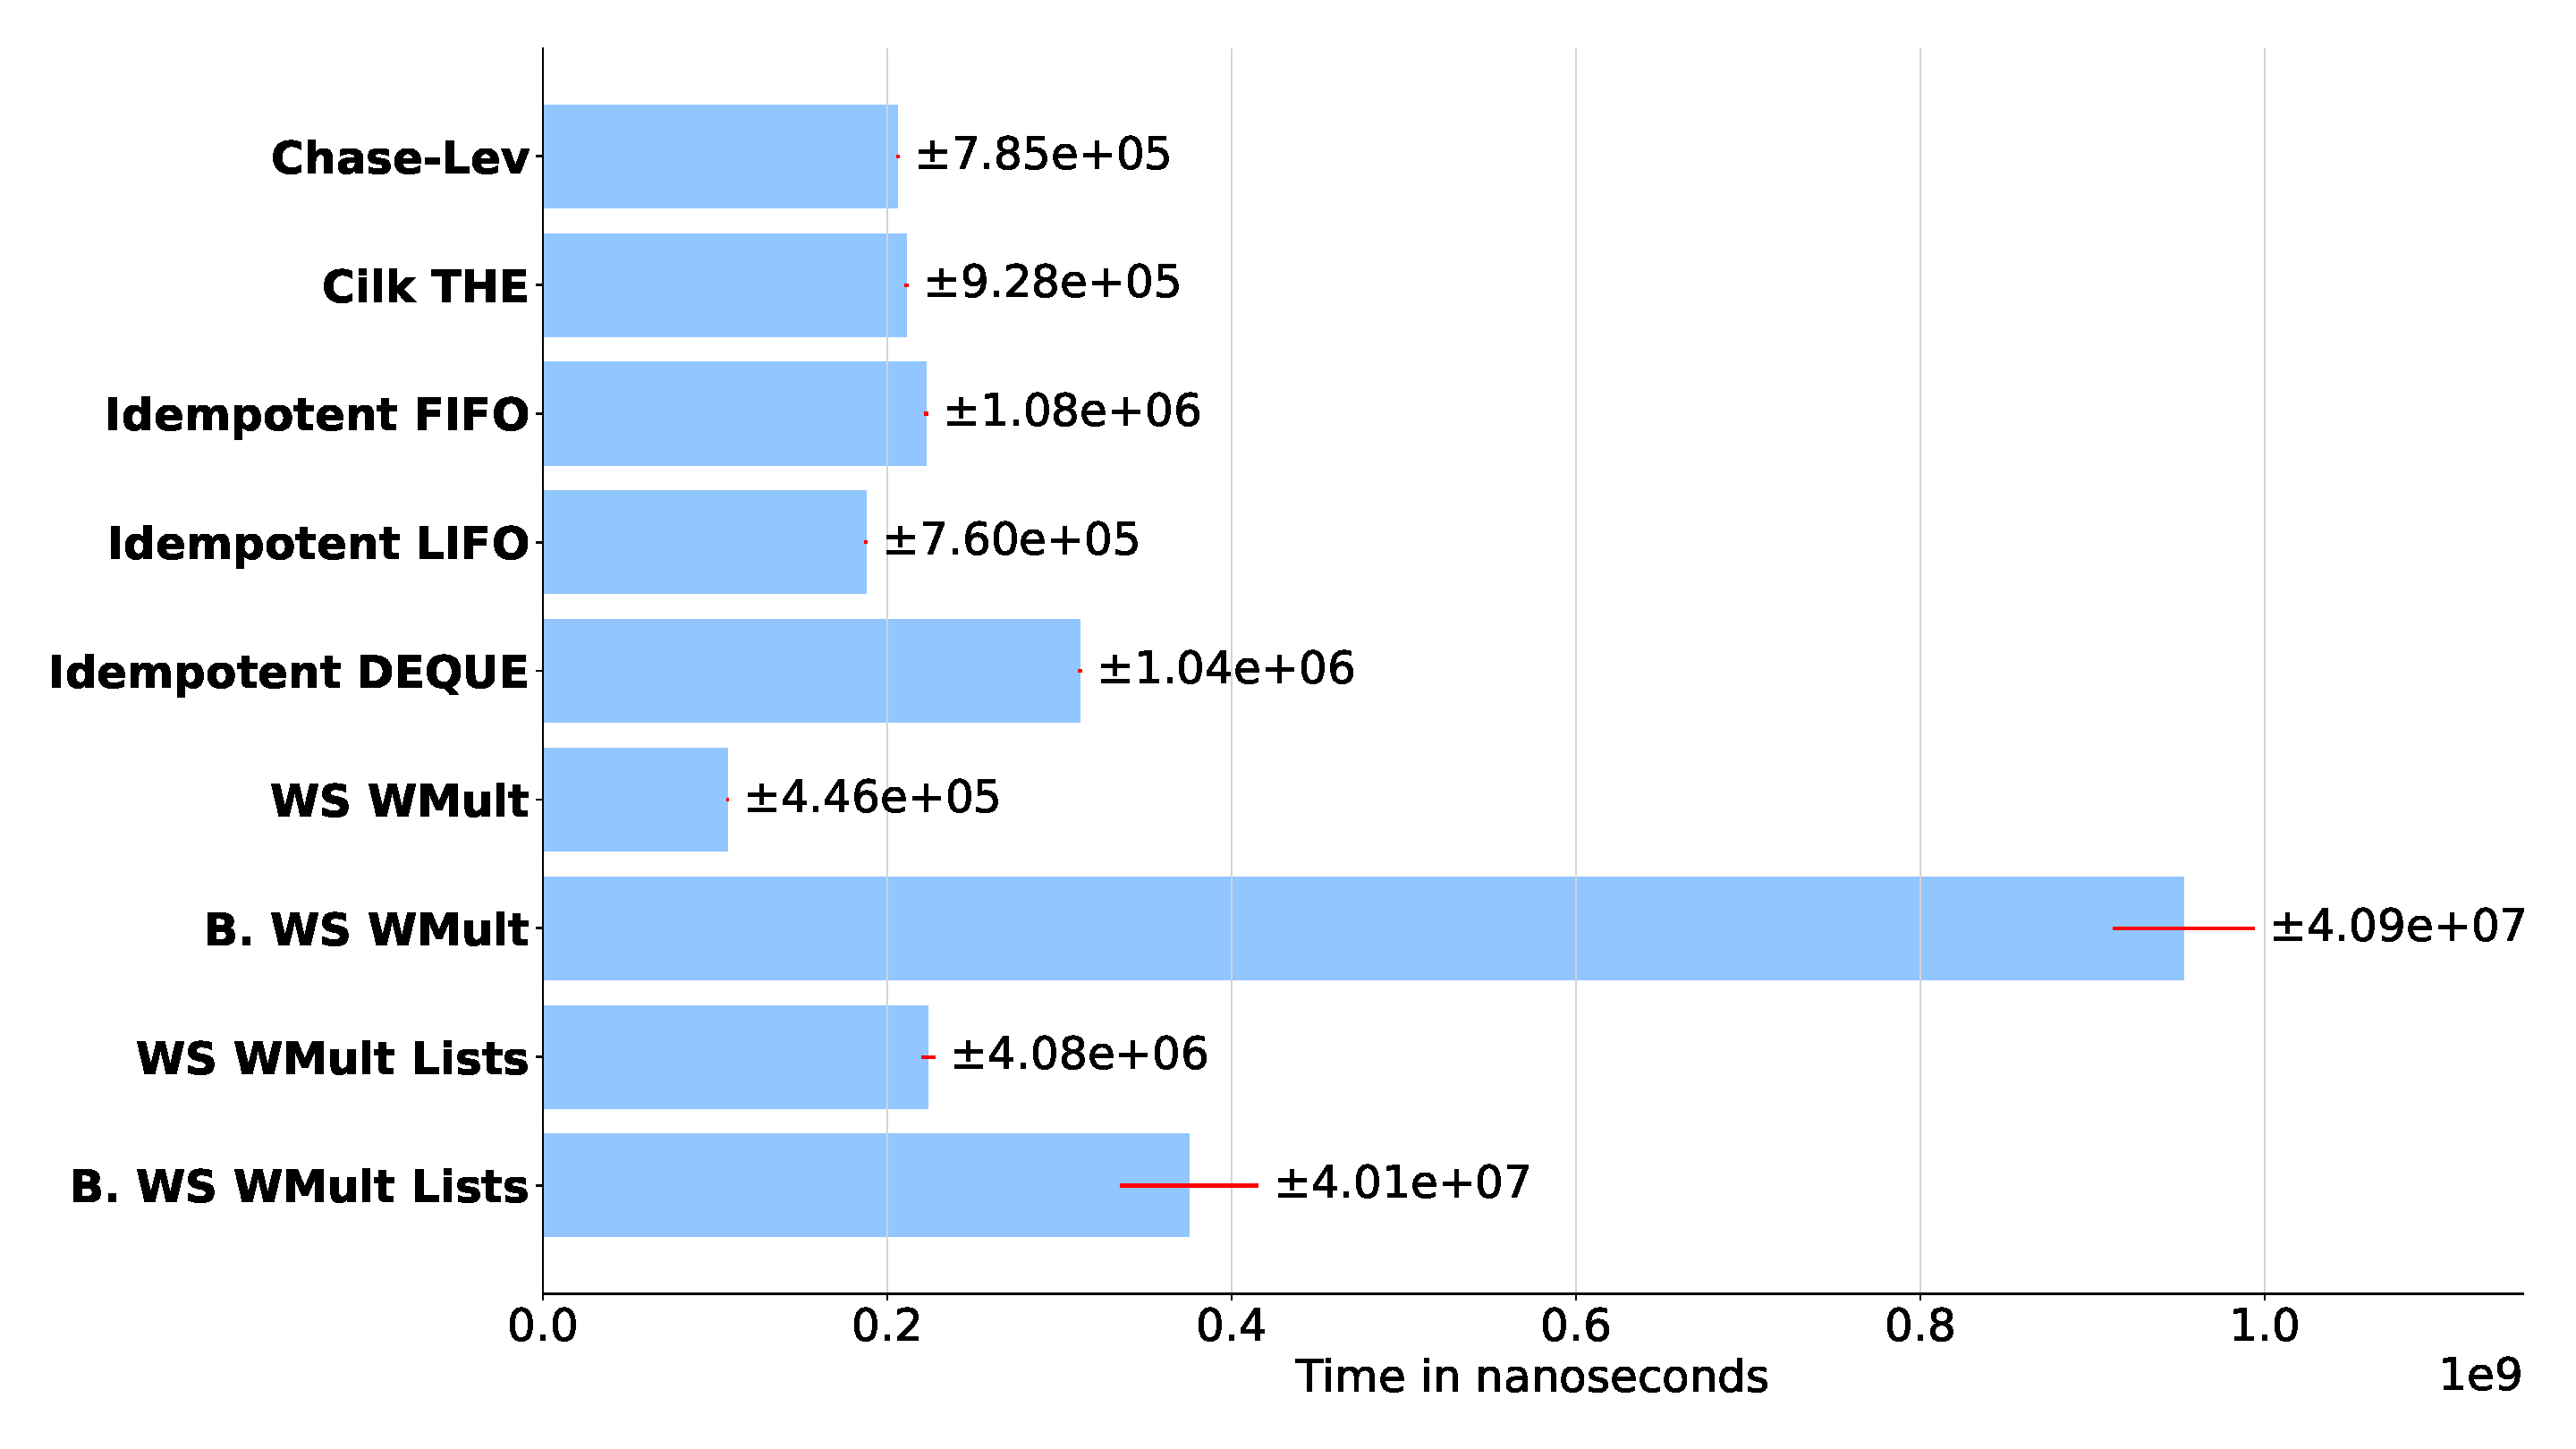
\includegraphics[width=0.47\textwidth]{contents/figures/IV_6_chart-puts-takes-256-10000000.pdf}
  }
  \subfloat[\label{fig:putstakes:1000000}Puts and Takes with an initial size 1,000,000]{
    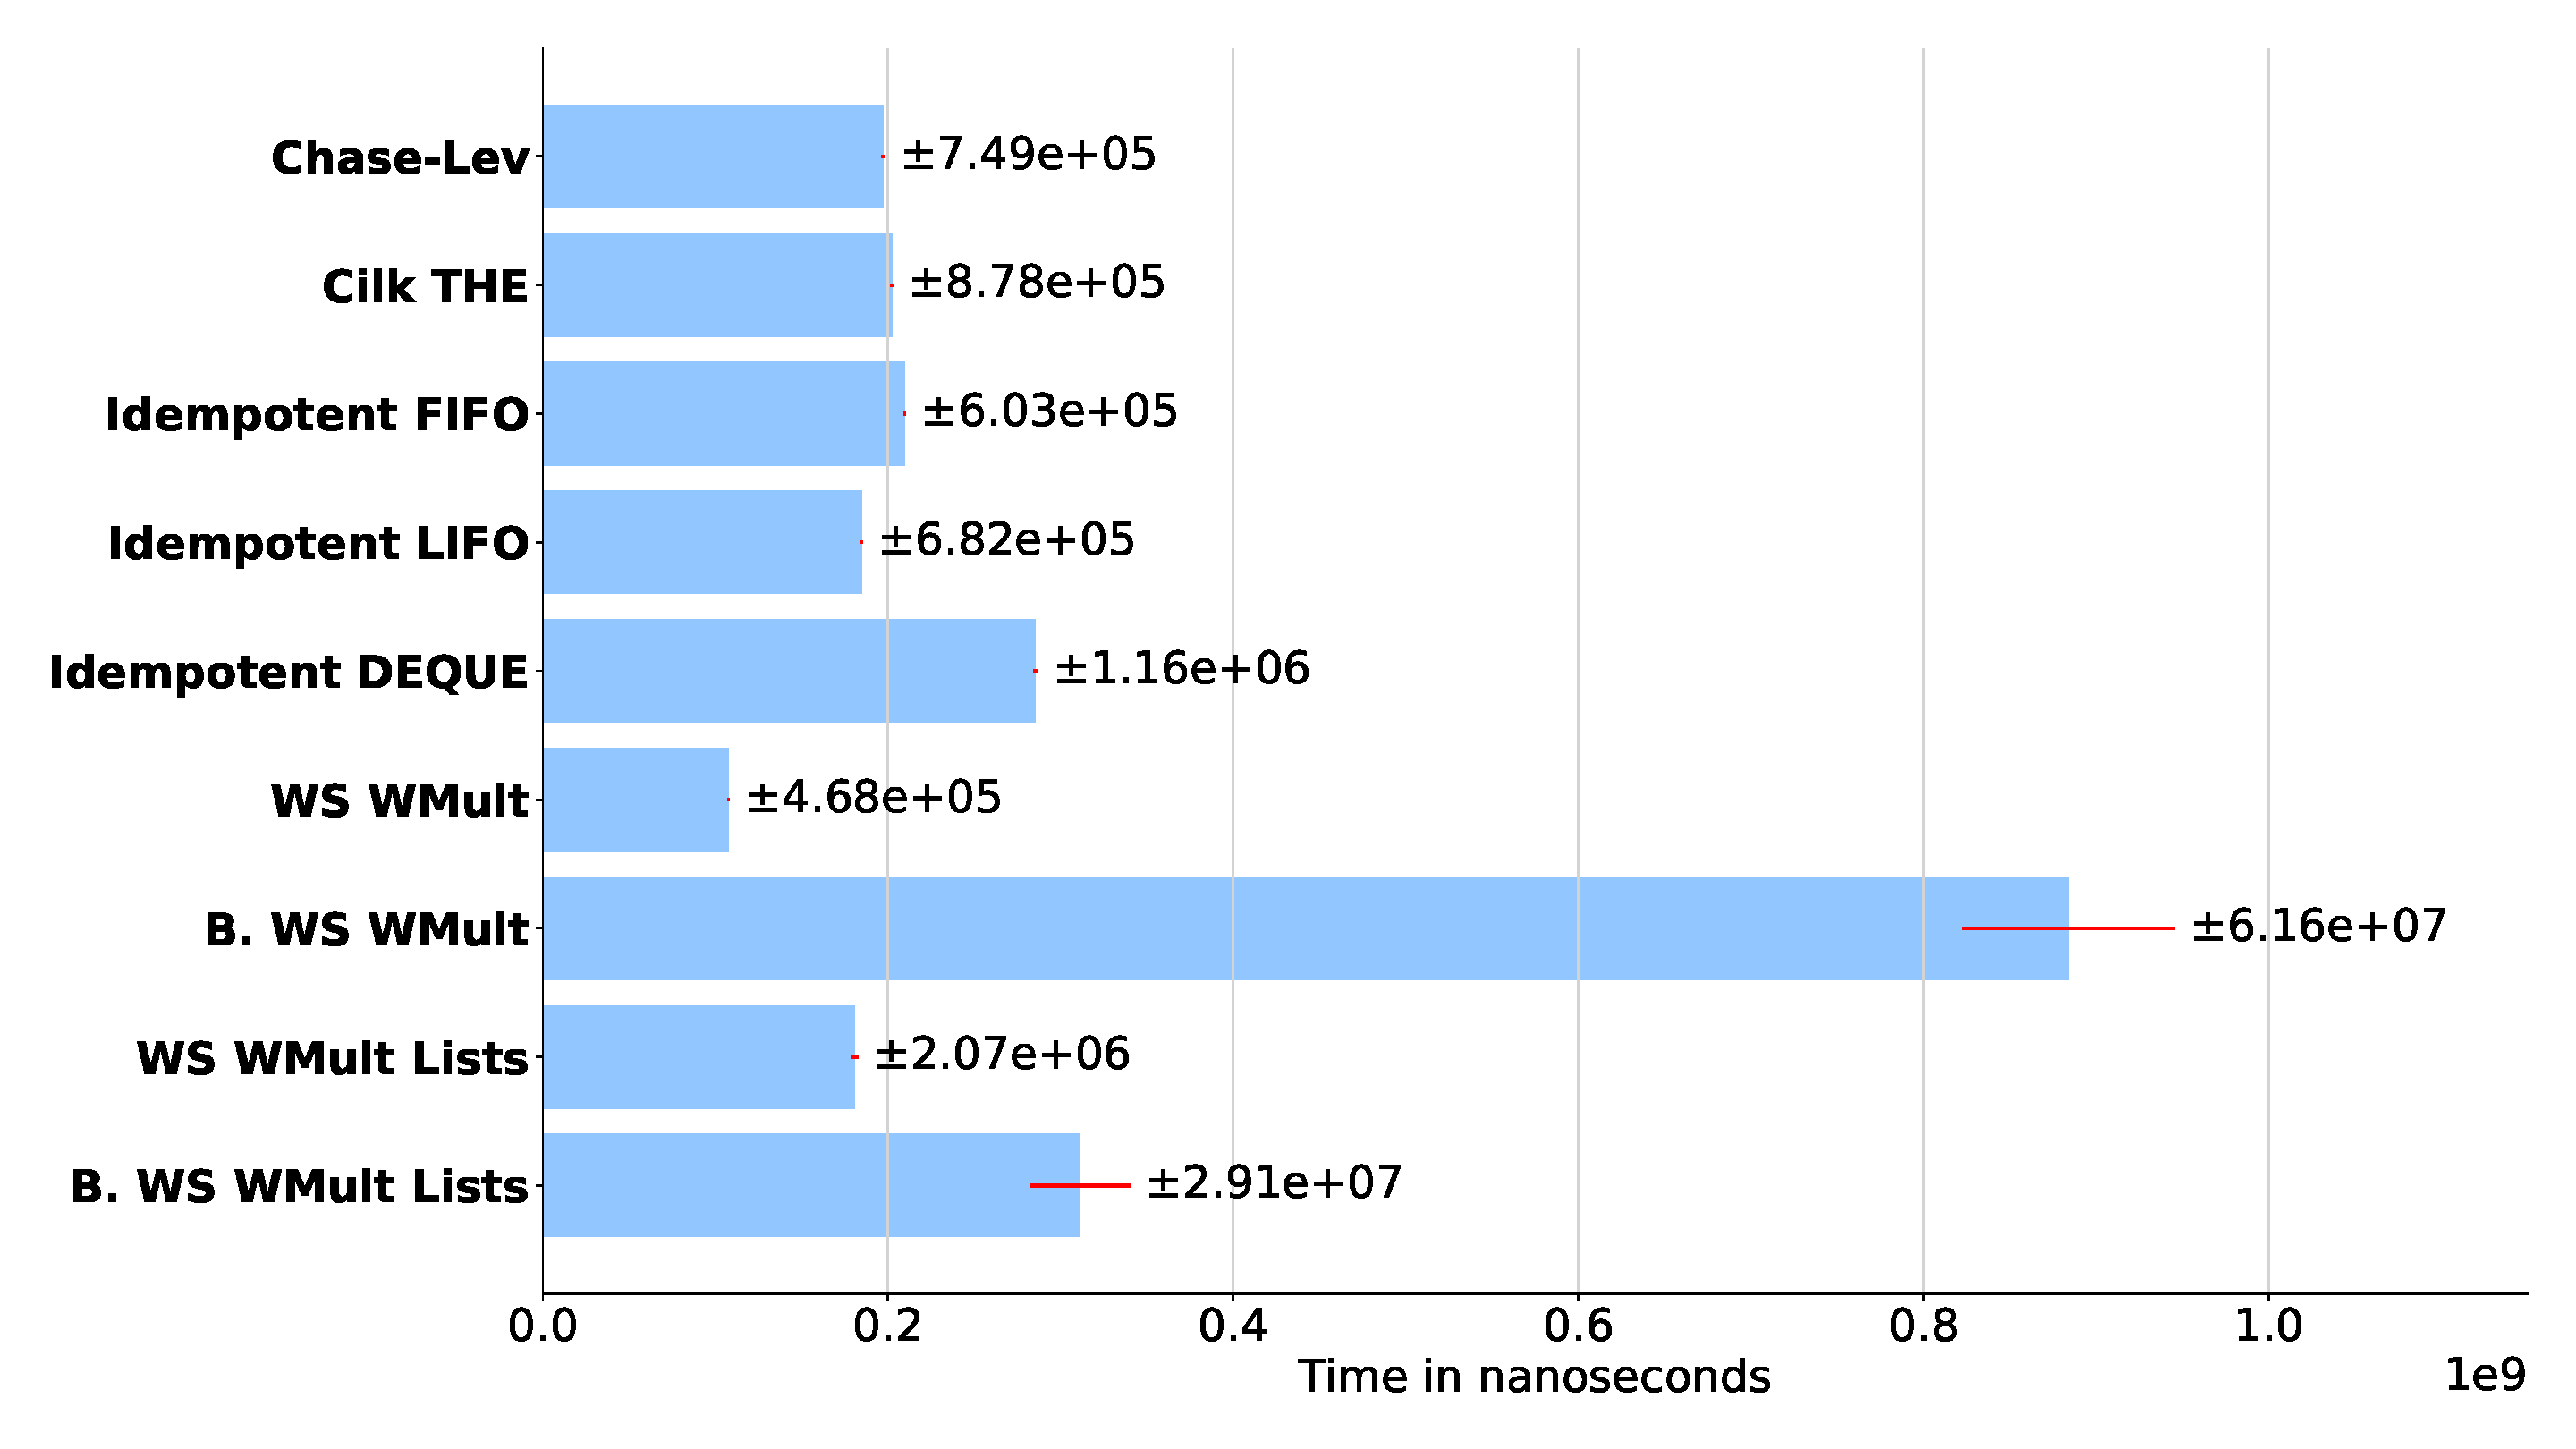
\includegraphics[width=0.47\textwidth]{contents/figures/IV_6_chart-puts-takes-1000000-10000000.pdf}
  }

  \subfloat[\label{fig:putstakes:10000000}Puts and Takes with an initial size 10,000,000]{
    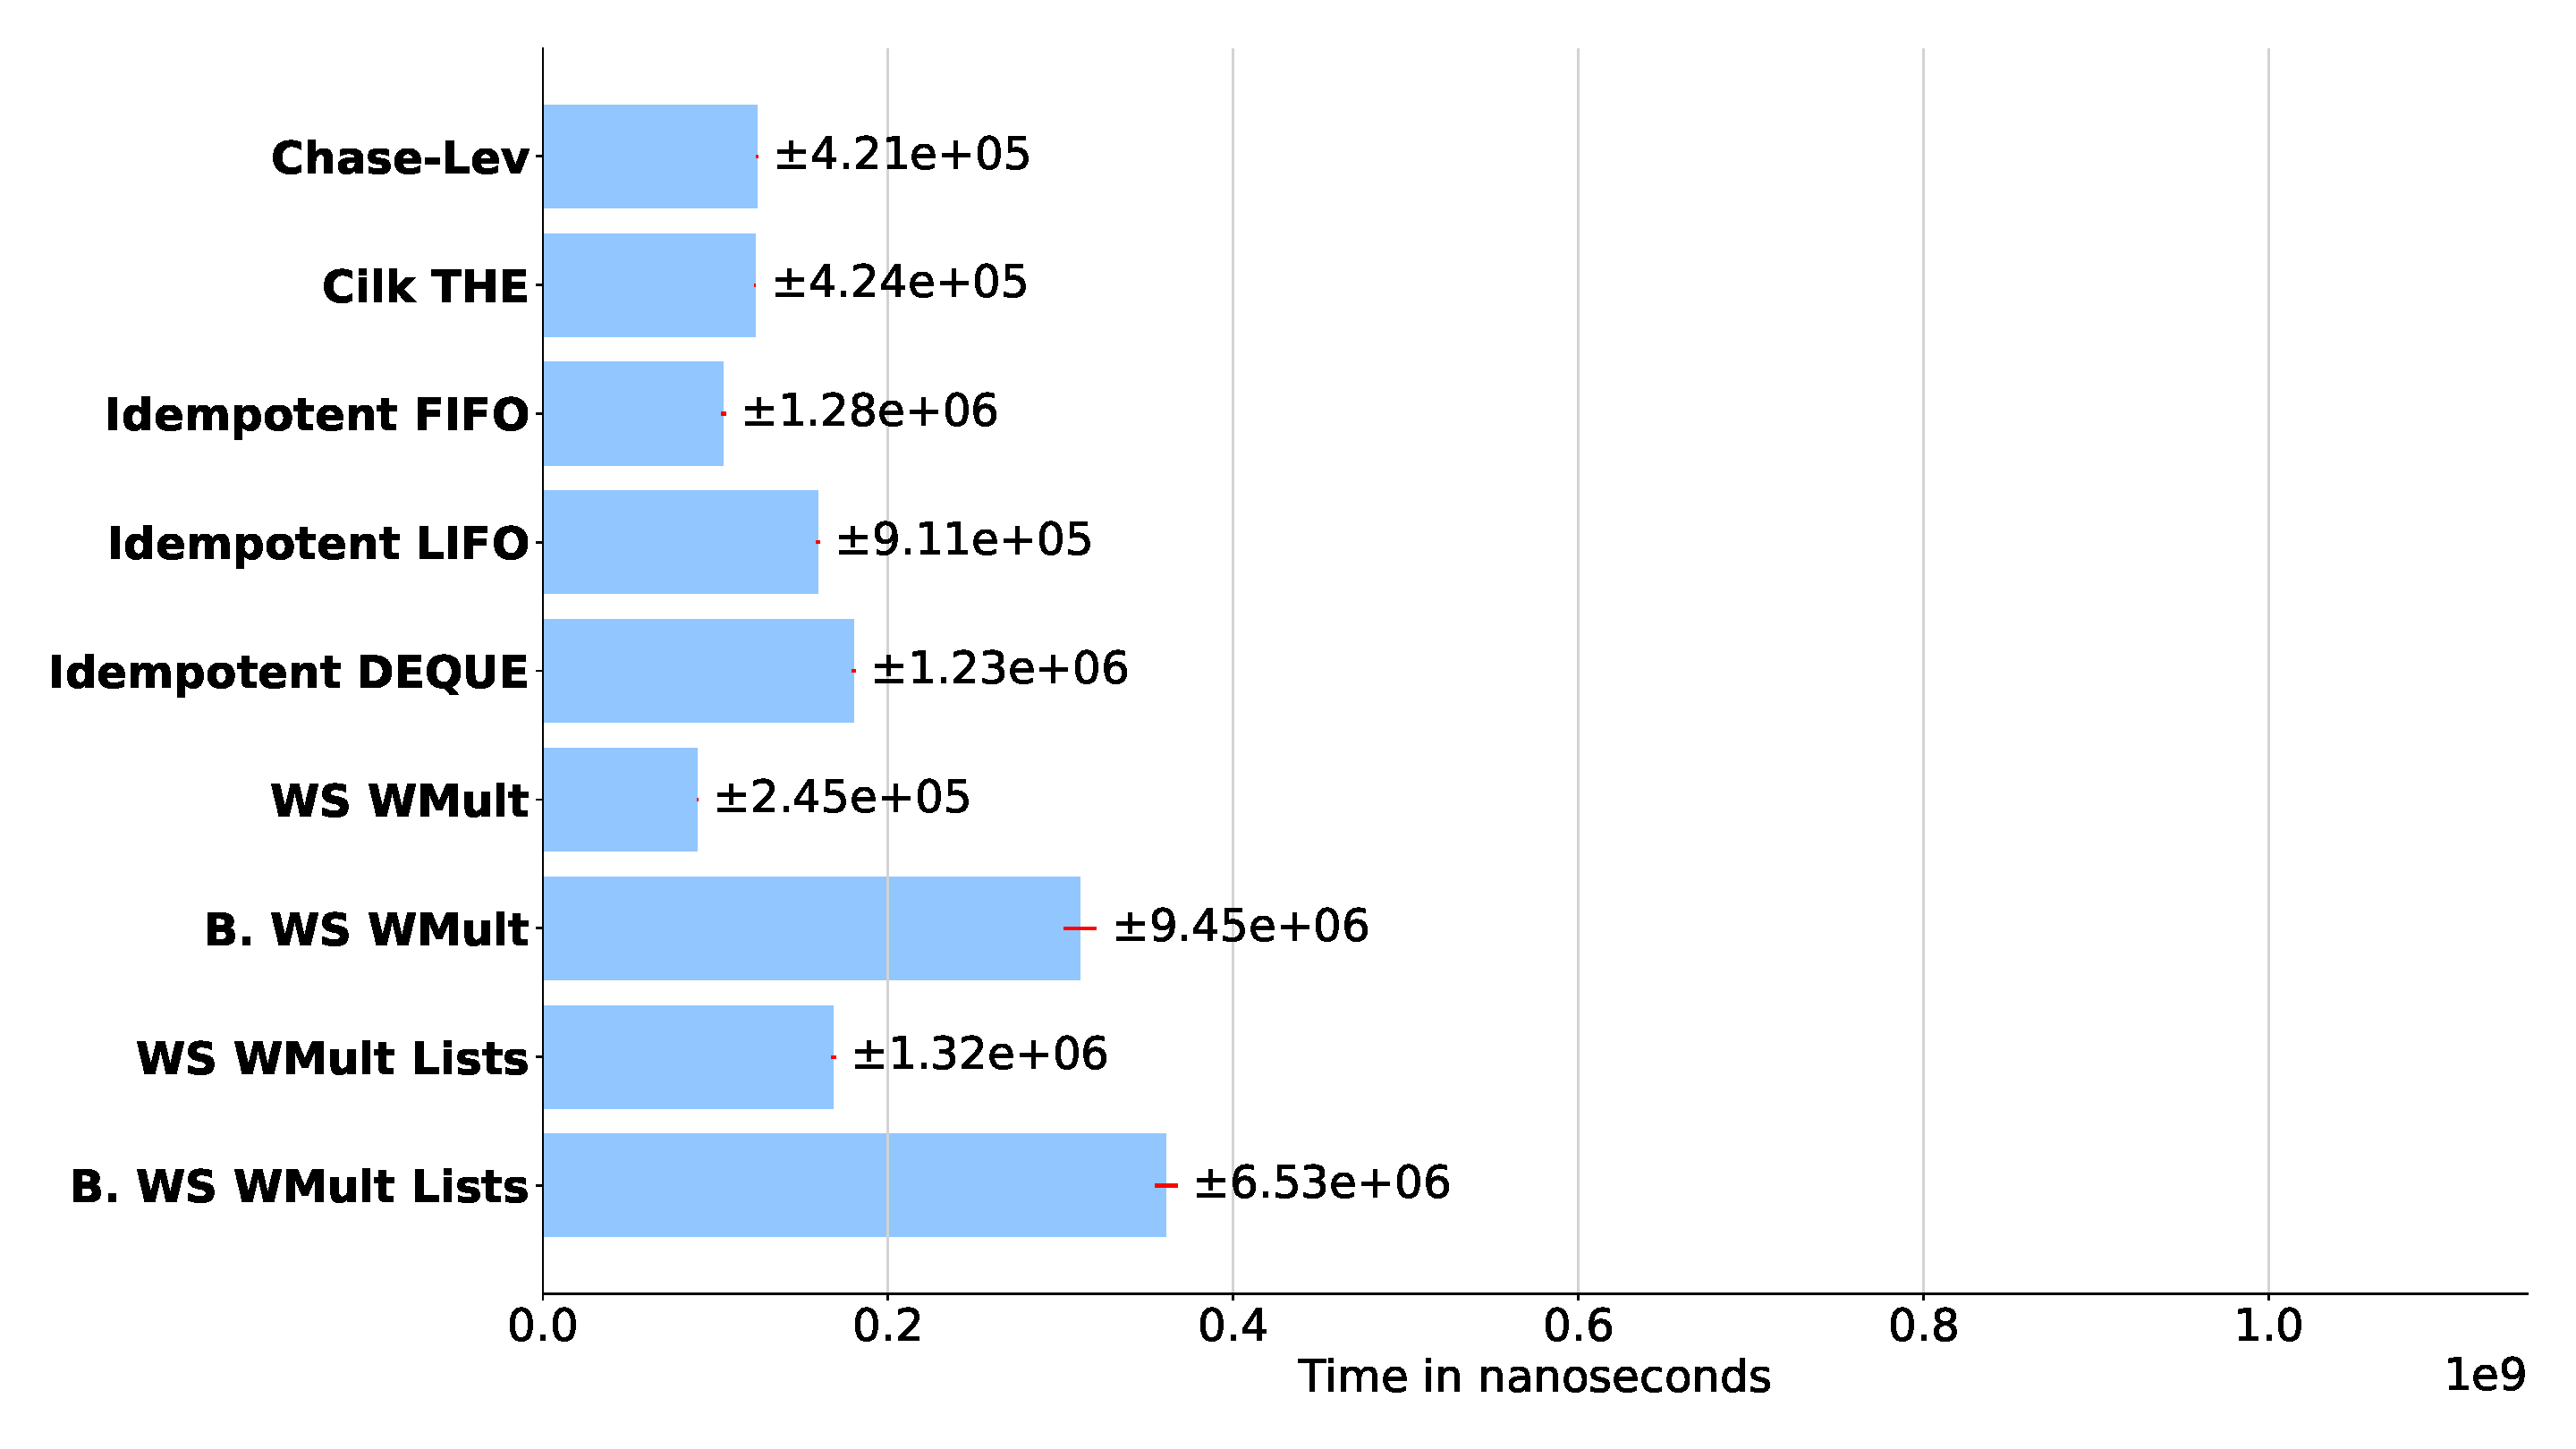
\includegraphics[width=0.47\textwidth]{contents/figures/IV_6_chart-puts-takes-10000000-10000000.pdf}
  }
  \subfloat[\label{fig:putssteals:256}Puts and Steals with an initial size 256]{
    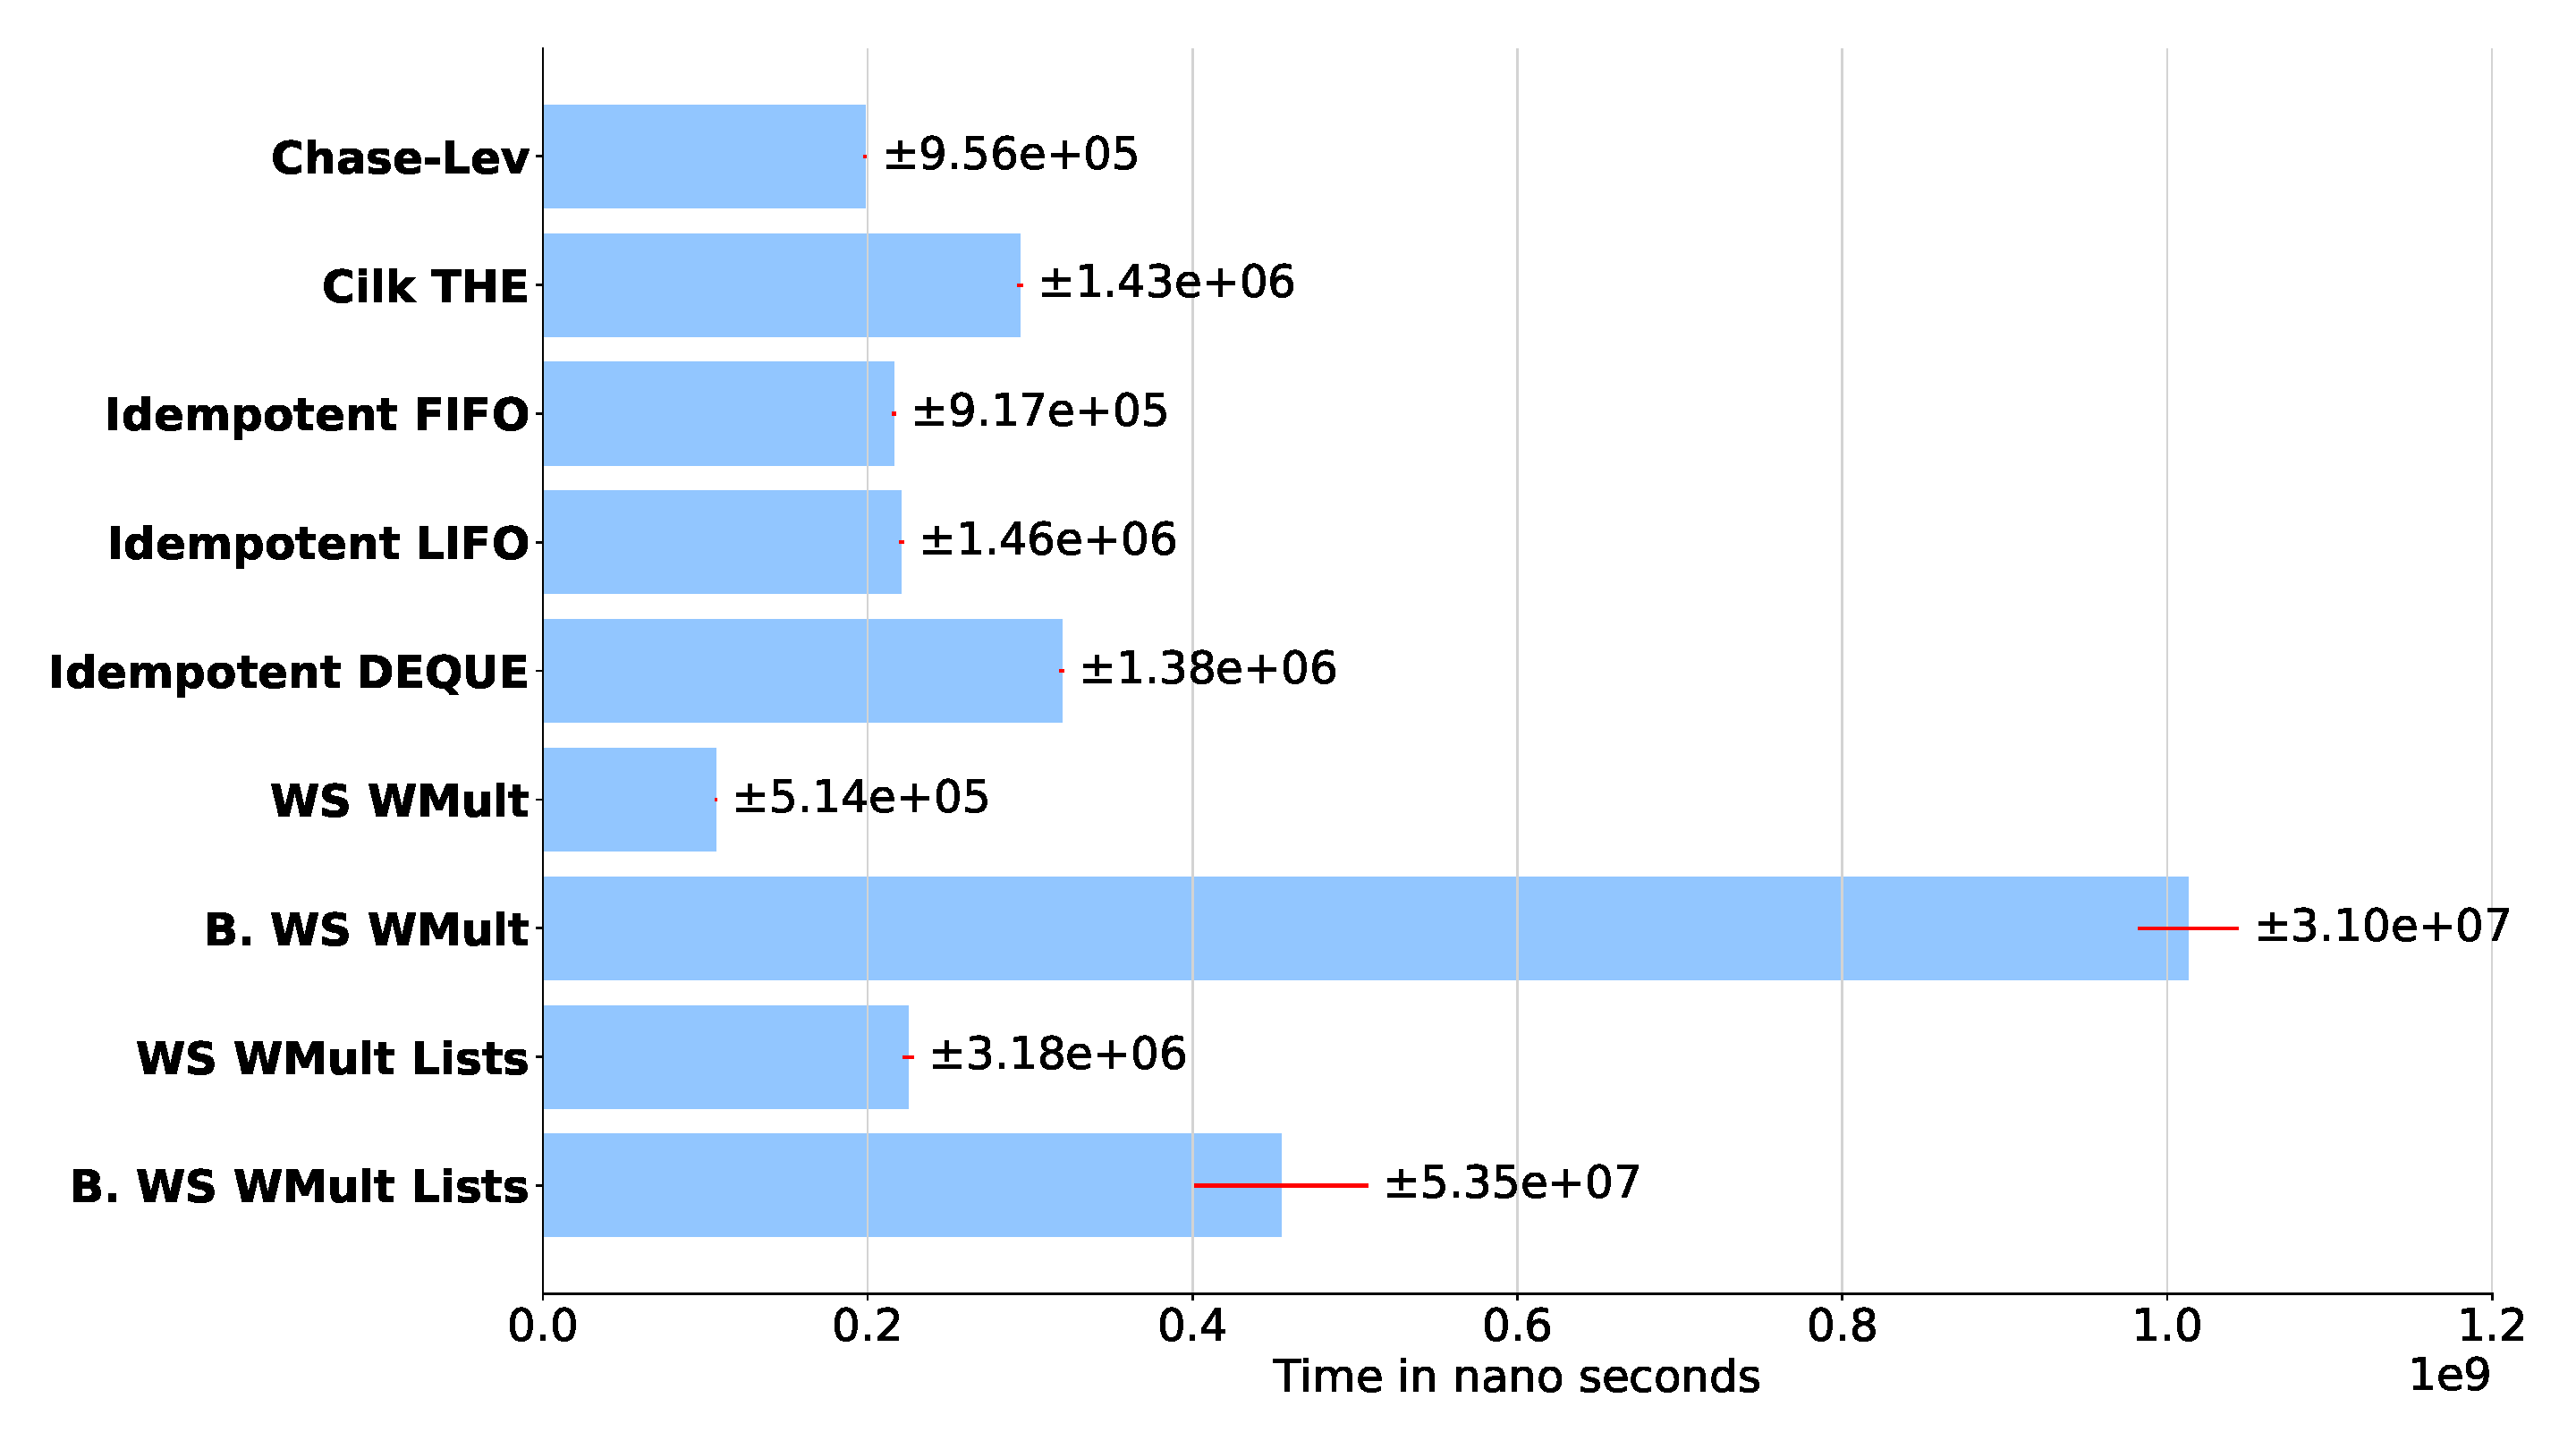
\includegraphics[width=0.47\textwidth]{contents/figures/IV_6_chart-puts-steals-256-10000000.pdf}
  }

  \subfloat[\label{fig:putssteals:1000000}Puts and Steals with an initial size 1,000,000]{
    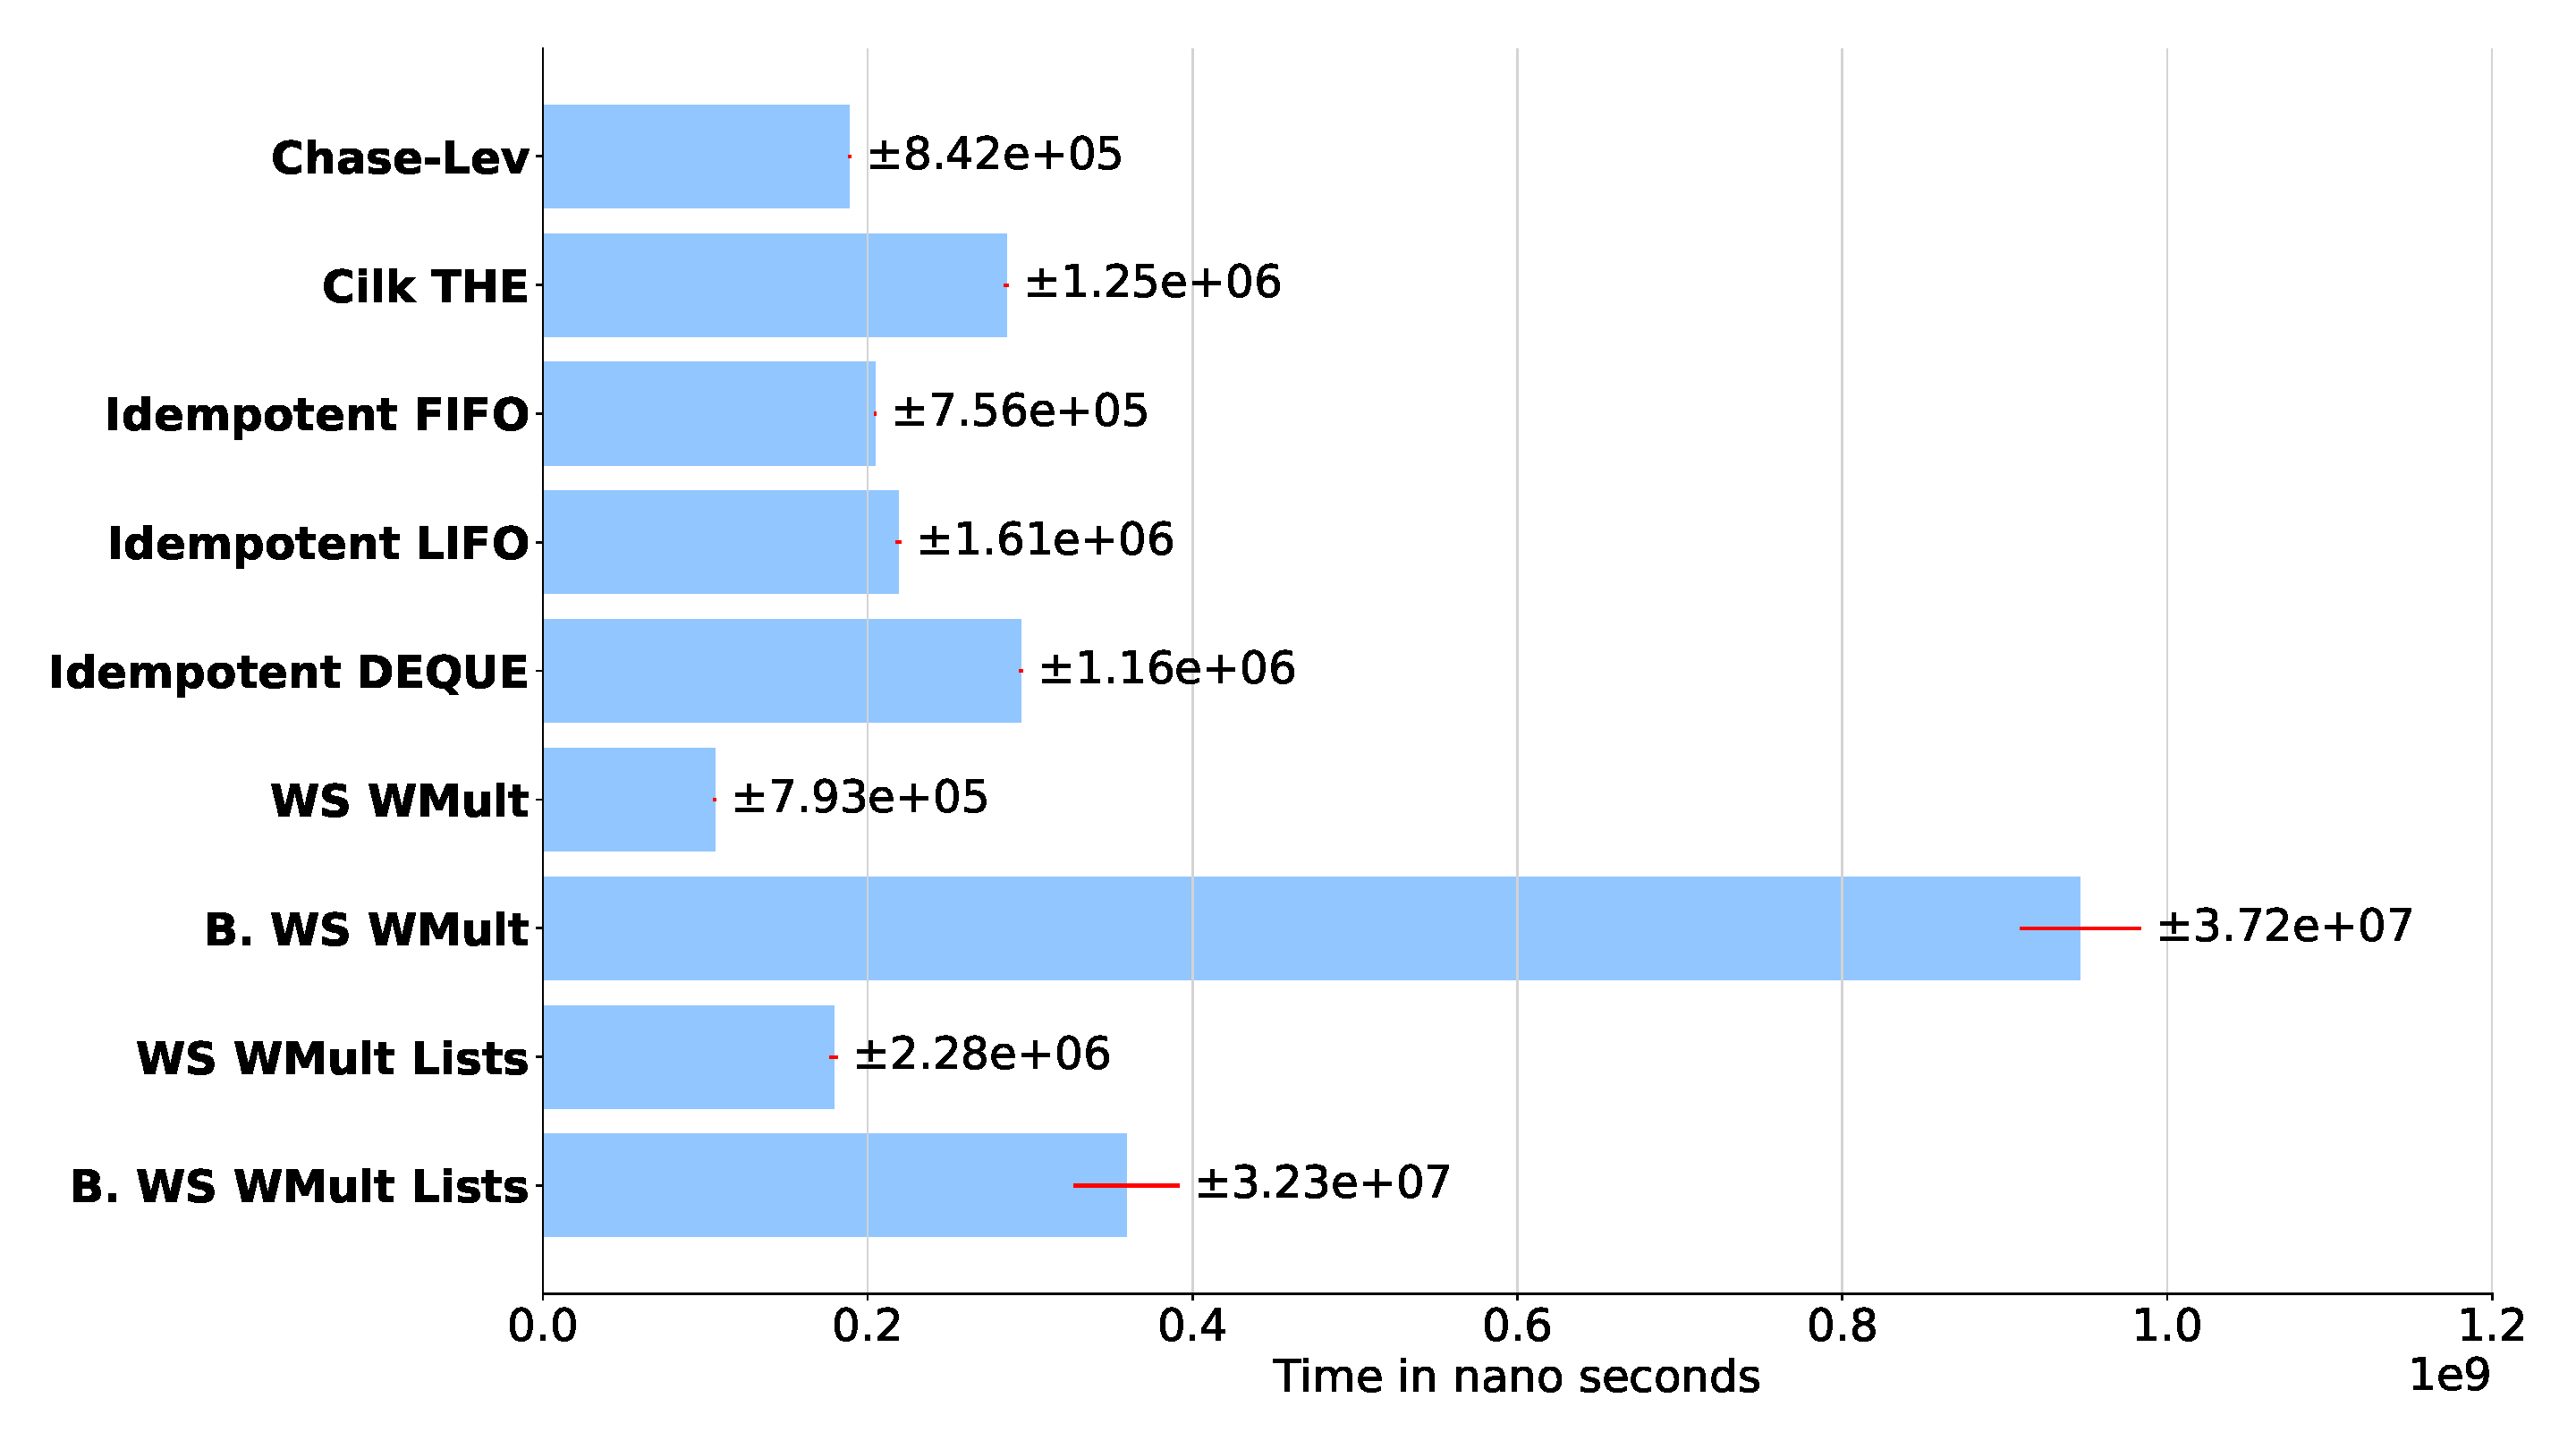
\includegraphics[width=0.47\textwidth]{contents/figures/IV_6_chart-puts-steals-1000000-10000000.pdf}

  }
  \subfloat[\label{fig:putssteals:10000000}Puts and Steals with an initial size 10,000,000]{
    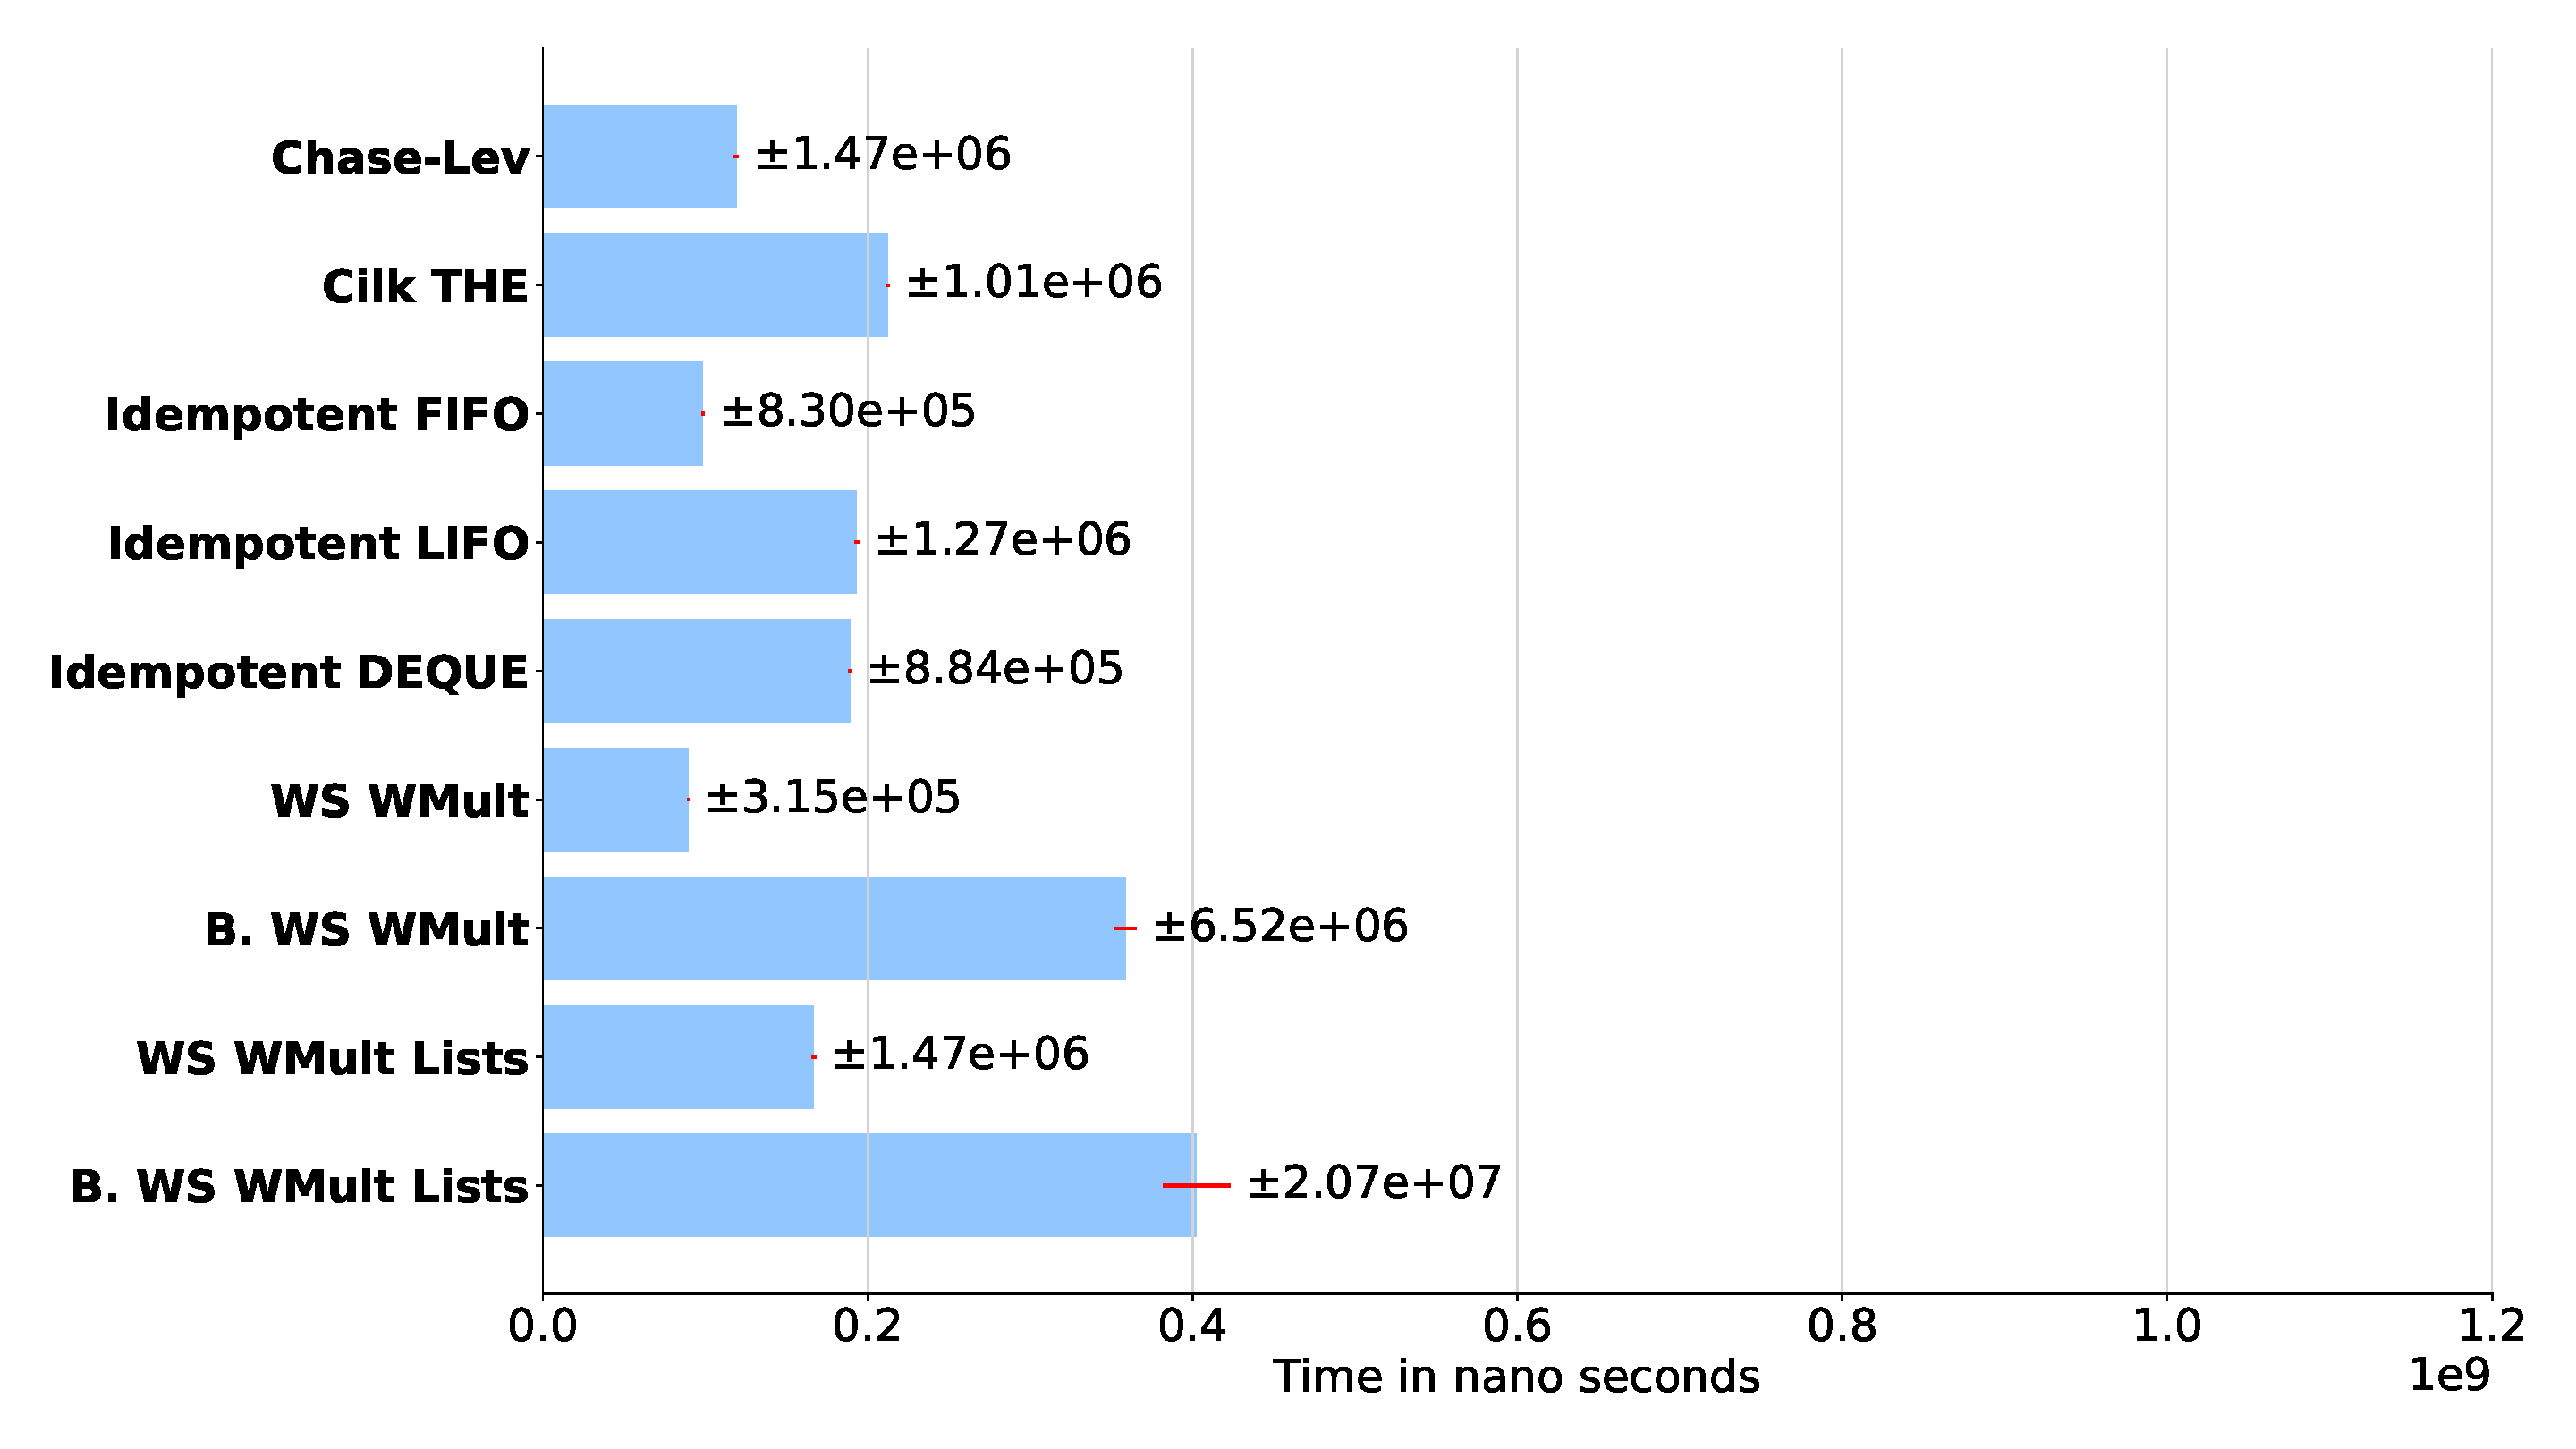
\includegraphics[width=0.4\textwidth]{contents/figures/IV_6_chart-puts-steals-10000000-10000000.pdf}
  }

  \caption{\label{fig:zerocost} Outcome of the zero cost experiments. Time is in nanoseconds, and red lines over bars show confidence intervals. The results of the $\Puts$-$\Takes$ experiment are shown in the first three charts and the results of the $\Puts$-$\Steals$ experiment are shown in the remaining charts.}

\end{figure}


\subsubsection{Parallel Spanning Tree}


Except for the case of Random graphs, where practically all algorithms performed equally, in general, \NCWSM{} outperformed all algorithms.  \NCWSM Lists and idempotent FIFO overall performed second and third best. The improvement of \NCWSM{} over \NCWSM Lists and idempotent FIFO was small, between 0.5\% and 4\%, depending on the graph. Thus, the absence of fences in \NCWSM{} resulted in a minor improvement over idempotent FIFO. It merits mentioning that \BNCWSM and its lists-based version generally showed a competitive performance, in some cases close to the first three algorithms. Usually, Cilk THE and Chase-Lev performed worst, which is expected as they use costly synchronization mechanisms, although this is not the only factor (more on this below).  \NCWSM outperformed Cilk THE by a margin between $1\%$ and $21\%$, and Chase-Lev by a margin between $0.14\%$ and $32\%$.  The lowest margins occurred in the case of Random graphs, where, as mentioned, all algorithms performed almost equally. Figure~\ref{fig:graphapplication} depicts the result of the experiment in some representative cases. In a few cases (e.g., Directed 2D Torus), Chase-Lev, Cilk THE, and idempotent LIFO performed best with few processes. This seems to be related to the topology of the graph and the algorithm's insert/extract task policy (the owner follows LIFO).

\begin{figure}[!ht]
  \subfloat[\label{fig:torus2ddirected:256}Graph: Directed Torus 2D. Initial size of 256 items]{
    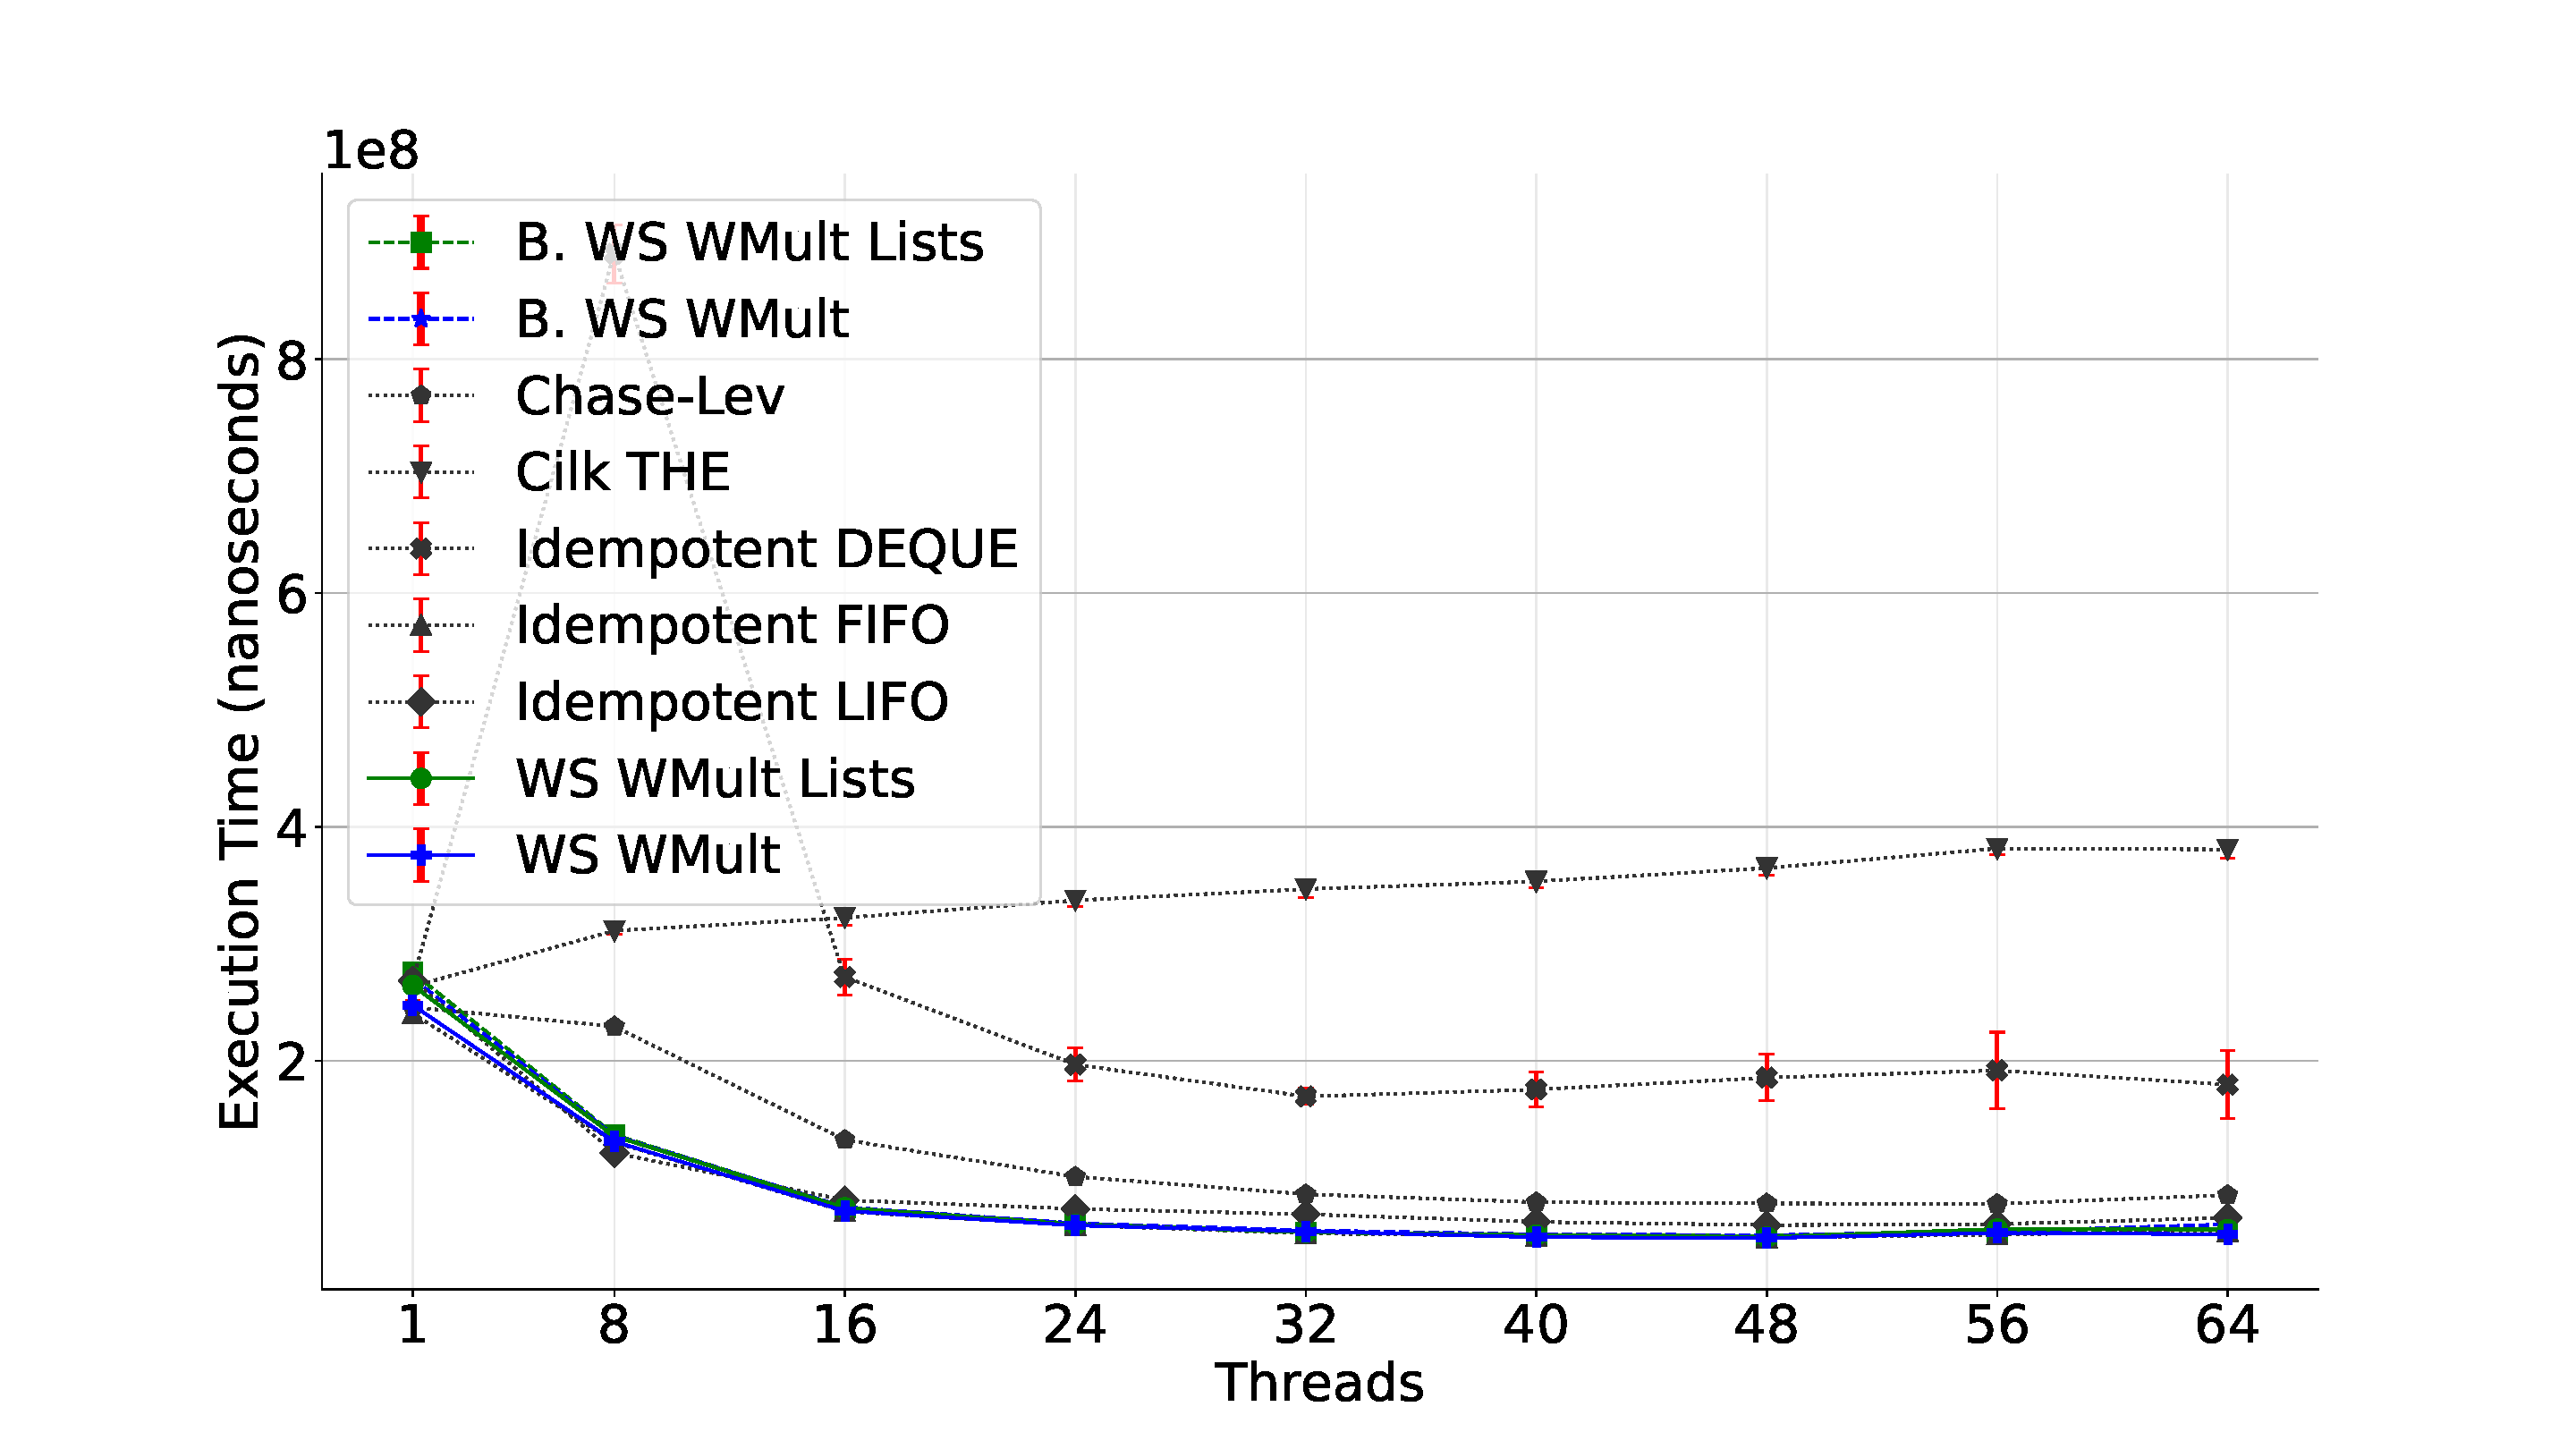
\includegraphics[width=0.48\textwidth]{contents/figures/IV_6_mean-TORUS2D-Directed-256.pdf}
  }
  \subfloat[\label{fig:torus2ddirected:1000000}Graph: Directed Torus 2D. Initial size of 1,000,000 items]{
    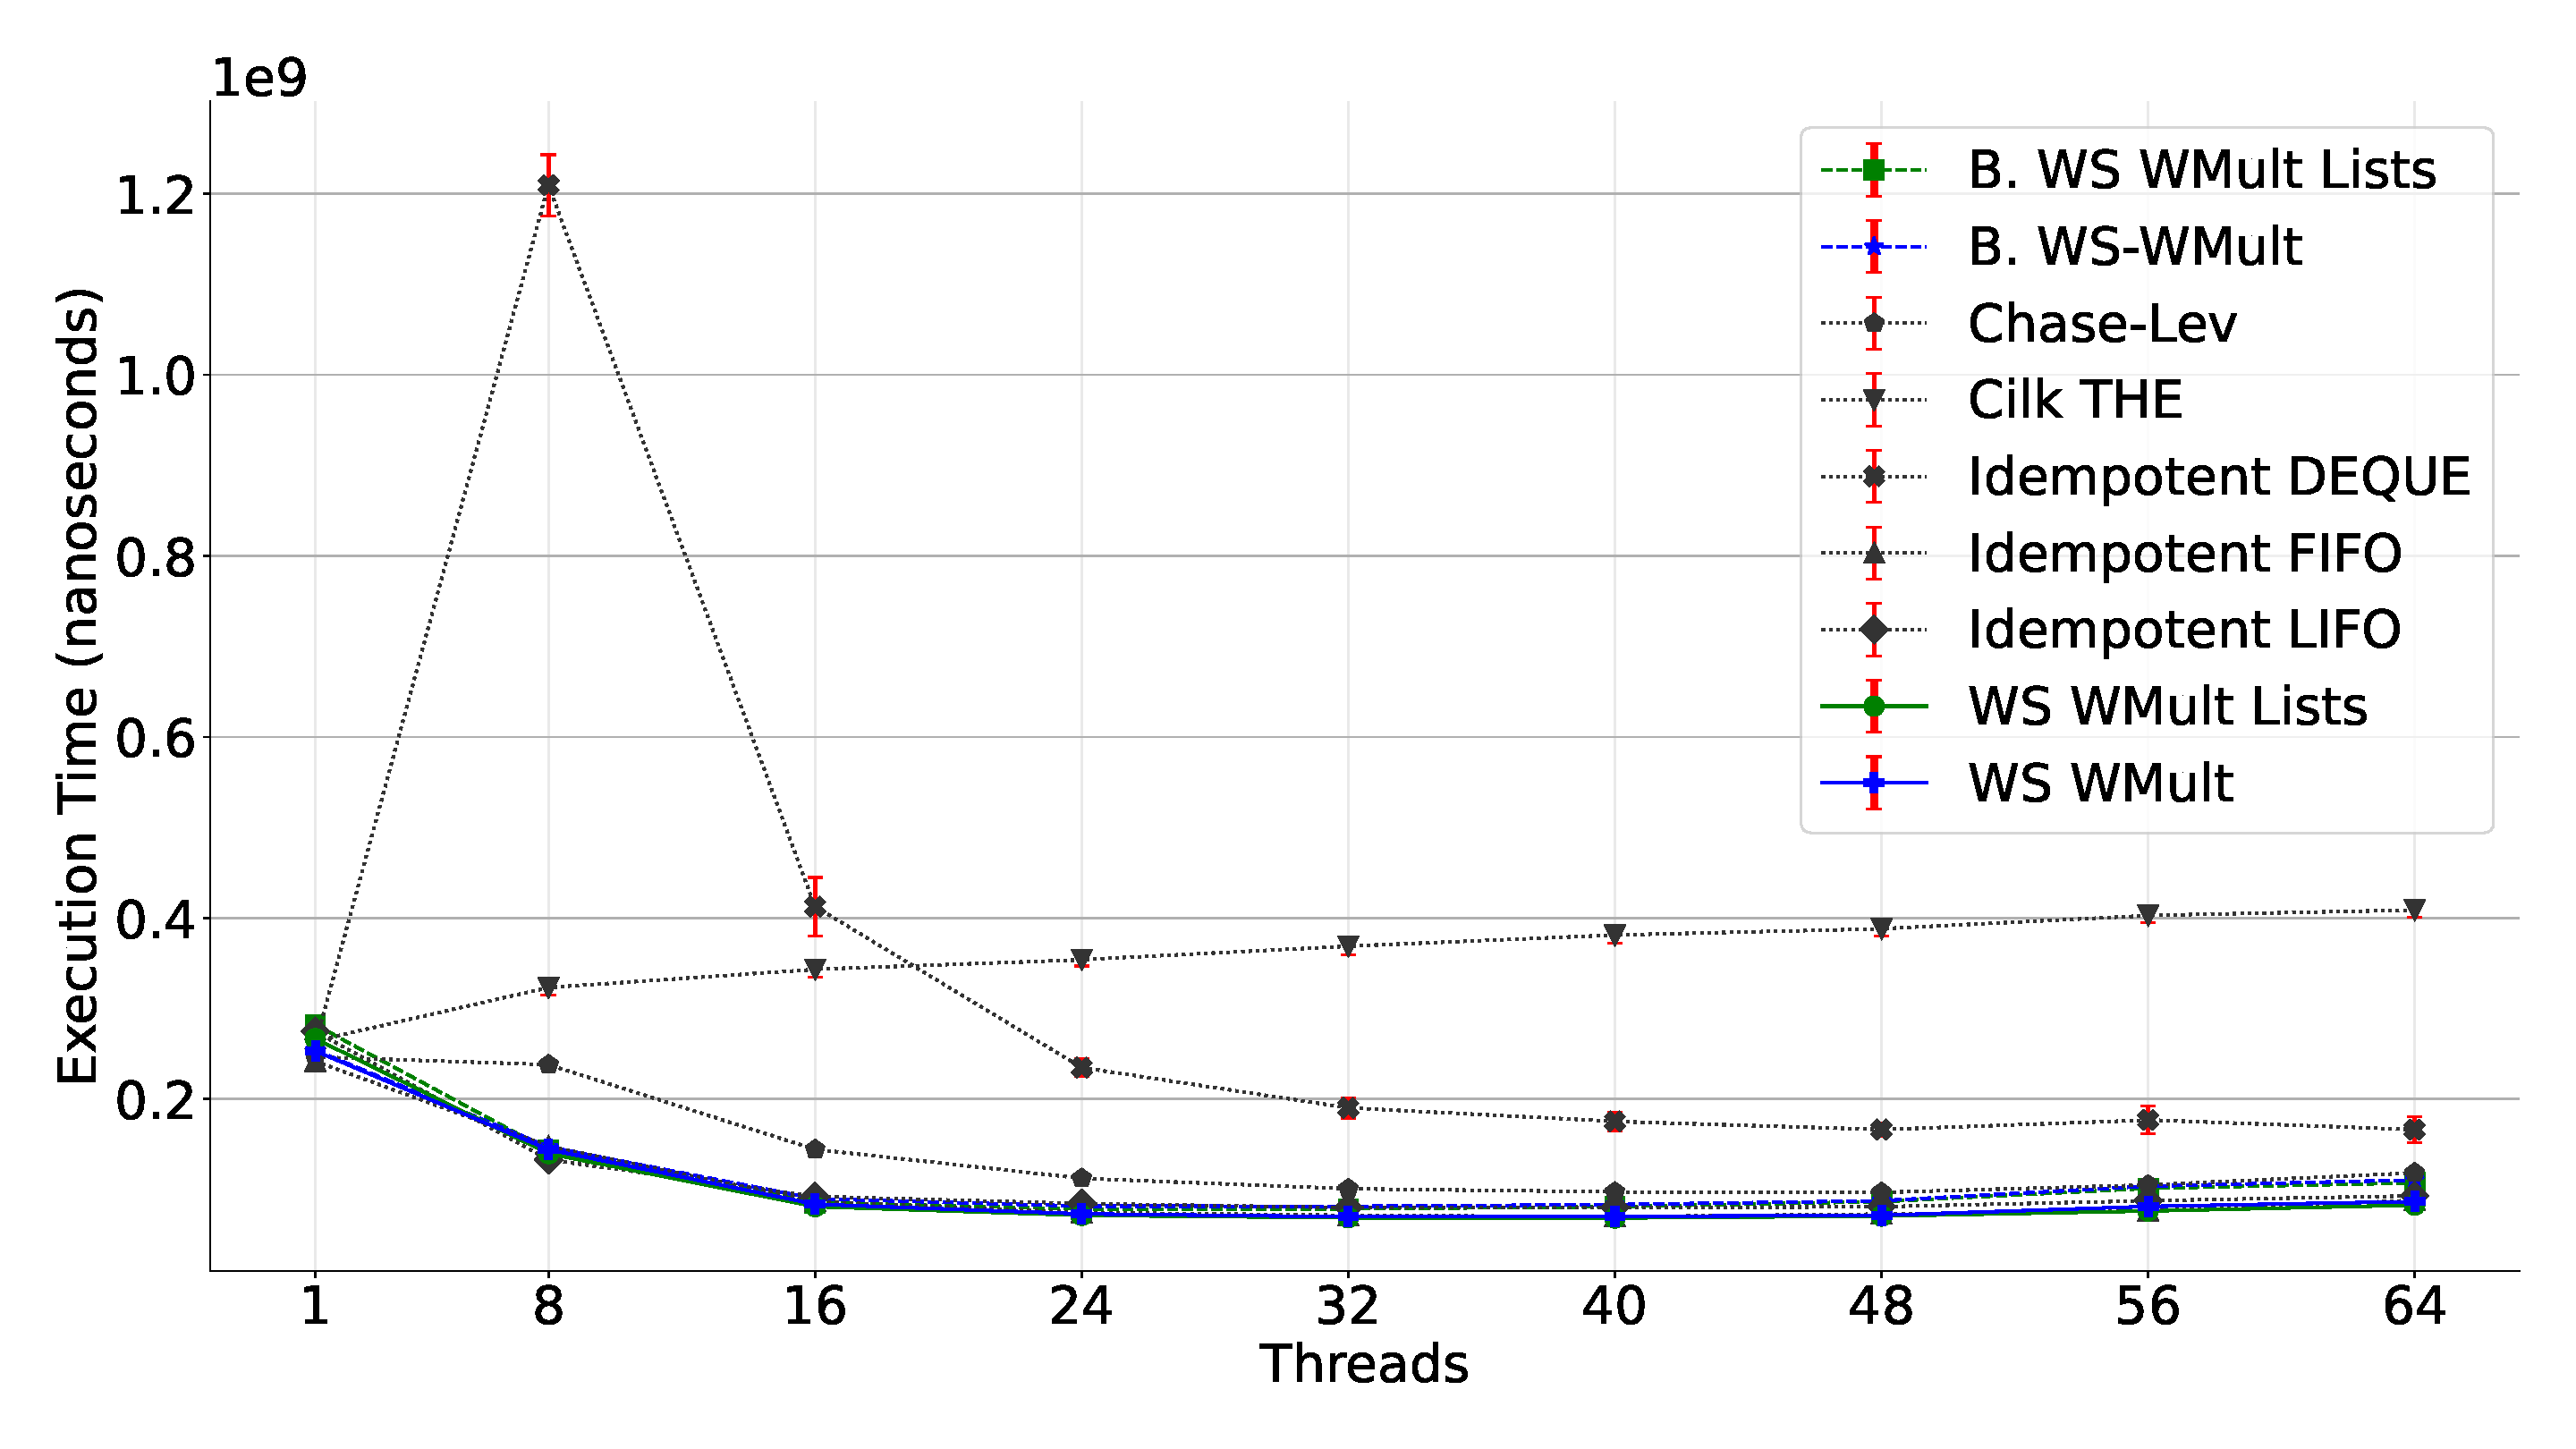
\includegraphics[width=0.48\textwidth]{contents/figures/IV_6_mean-TORUS2D-Directed-1000000.pdf}
  }

  \subfloat[\label{fig:torus3ddirected:256}Graph: Directed Torus 3D. Initial size of 256 items]{
    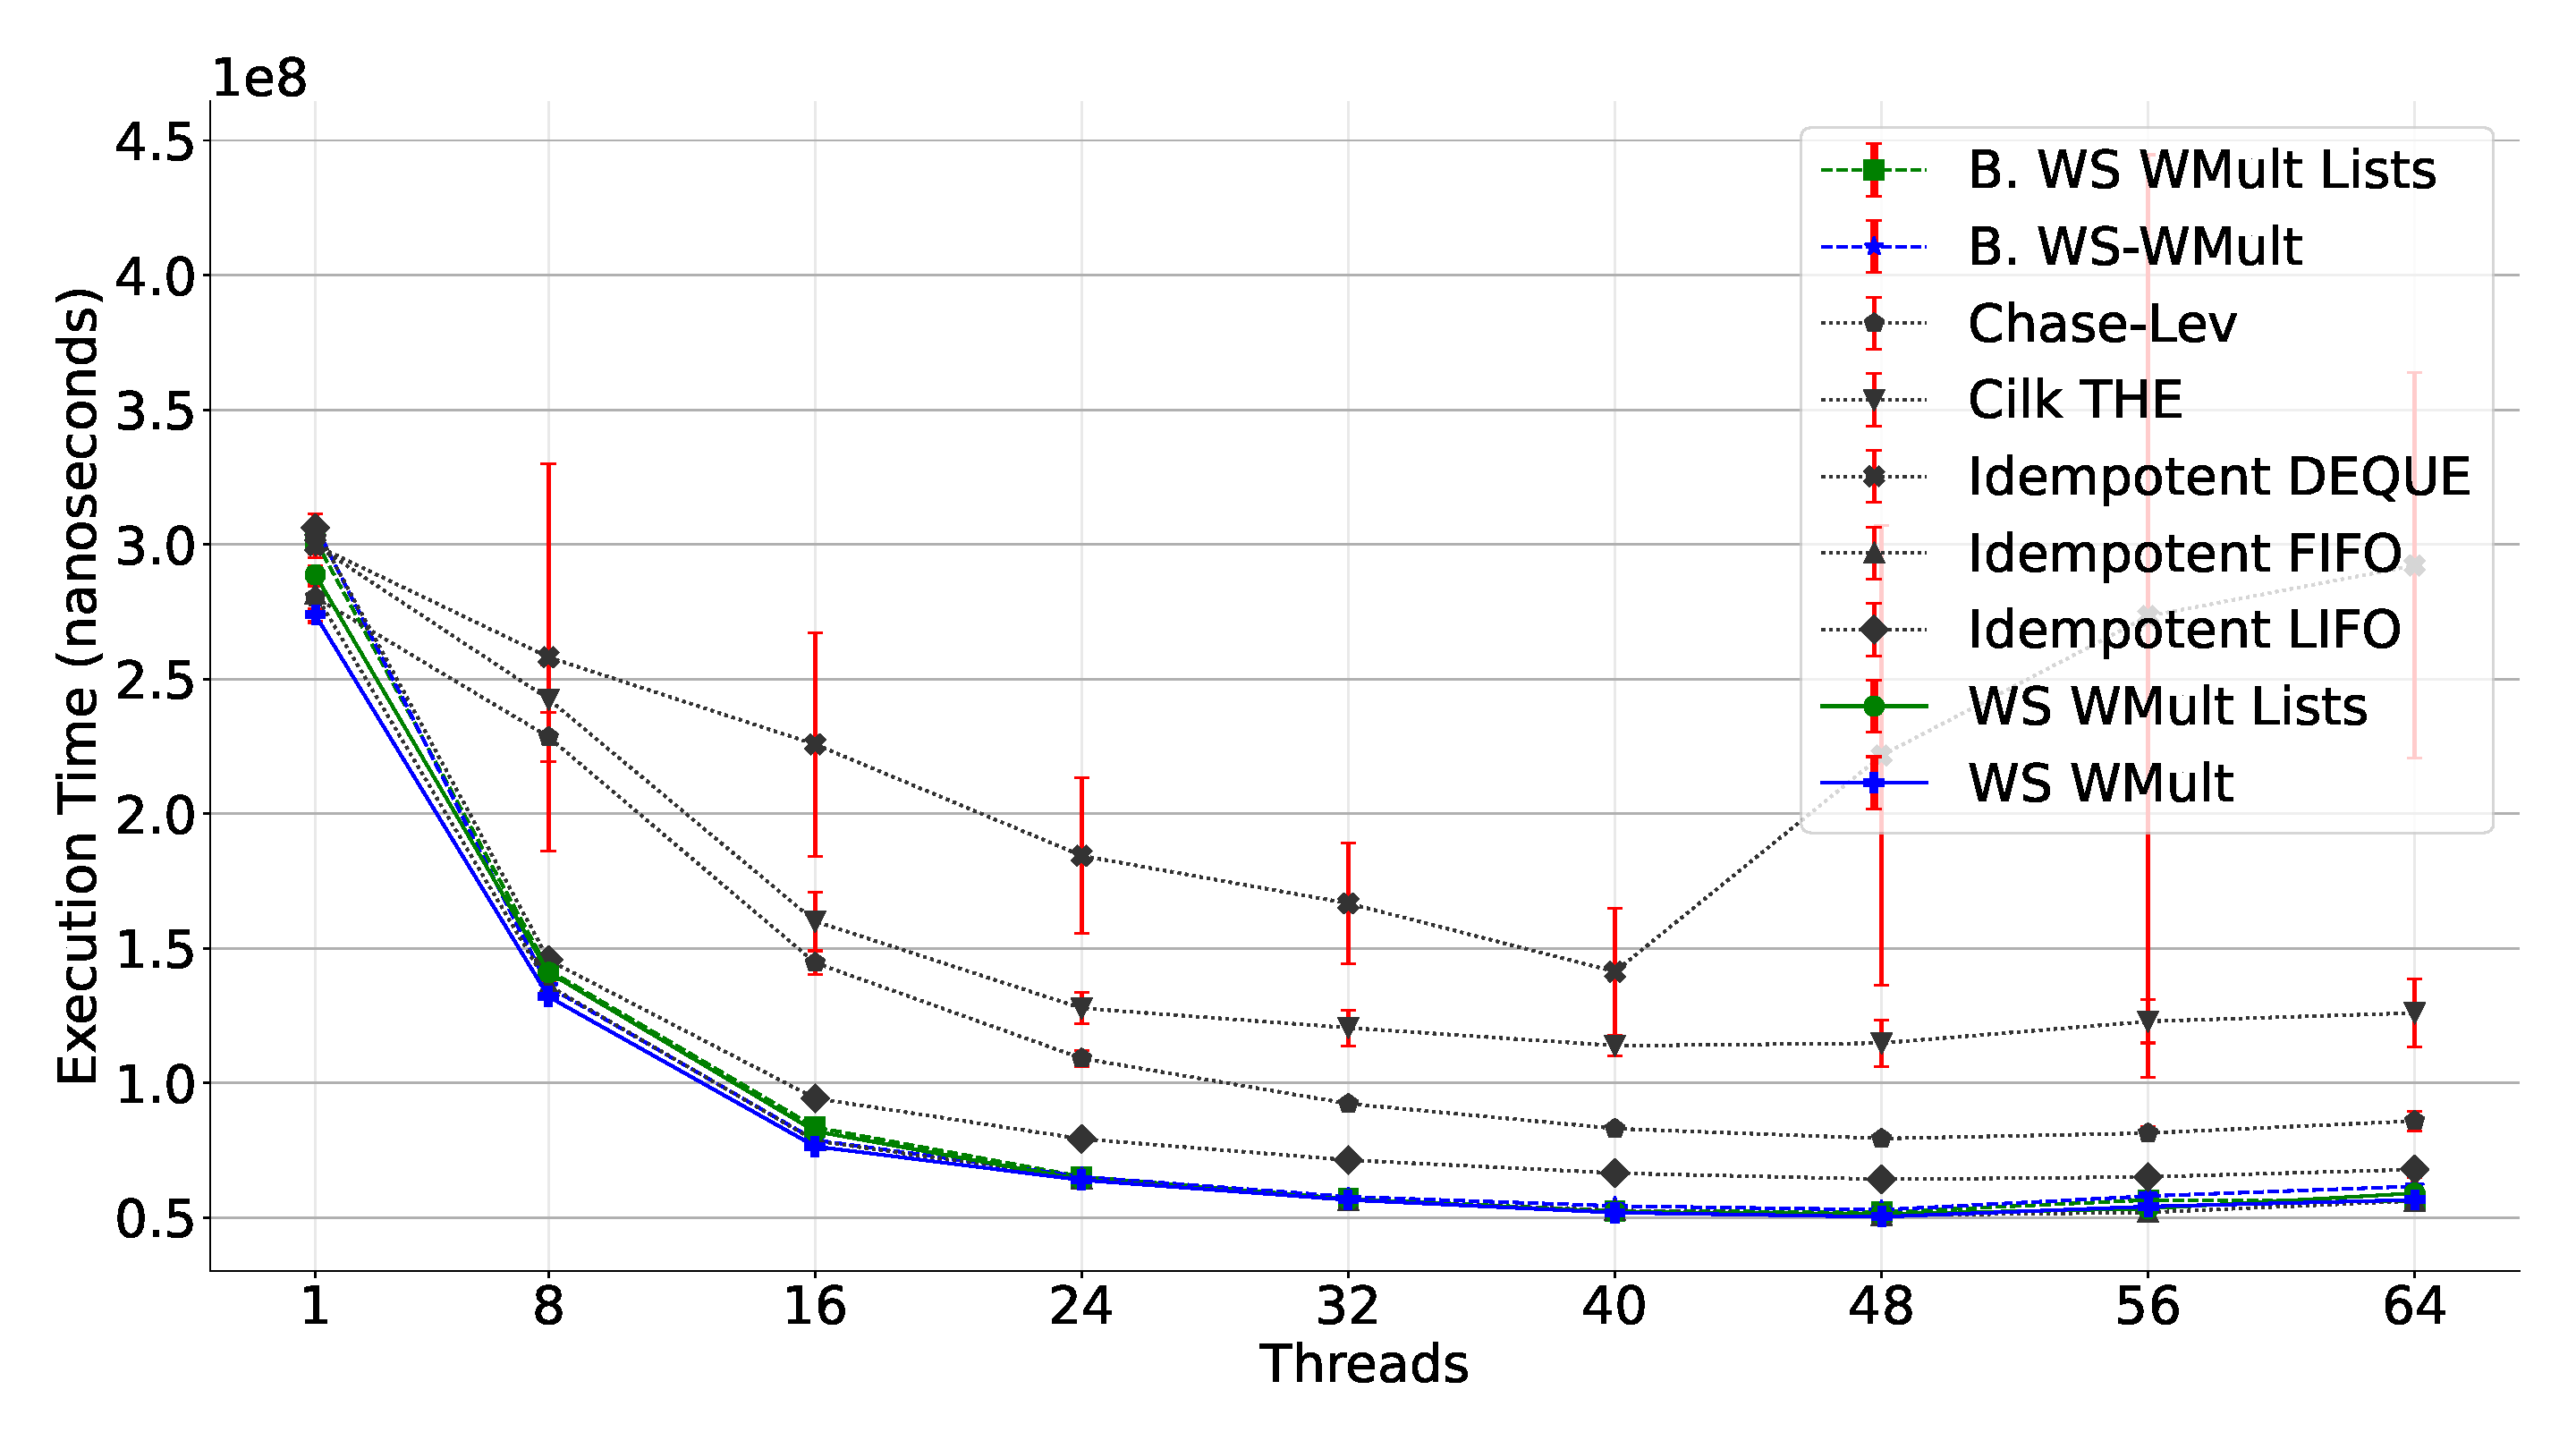
\includegraphics[width=0.48\textwidth]{contents/figures/IV_6_mean-TORUS3D-Directed-256.pdf}
  }
  \subfloat[\label{fig:torus3ddirected:1000000}Graph: Directed Torus 3D. Initial size of 1,000,000 items]{
    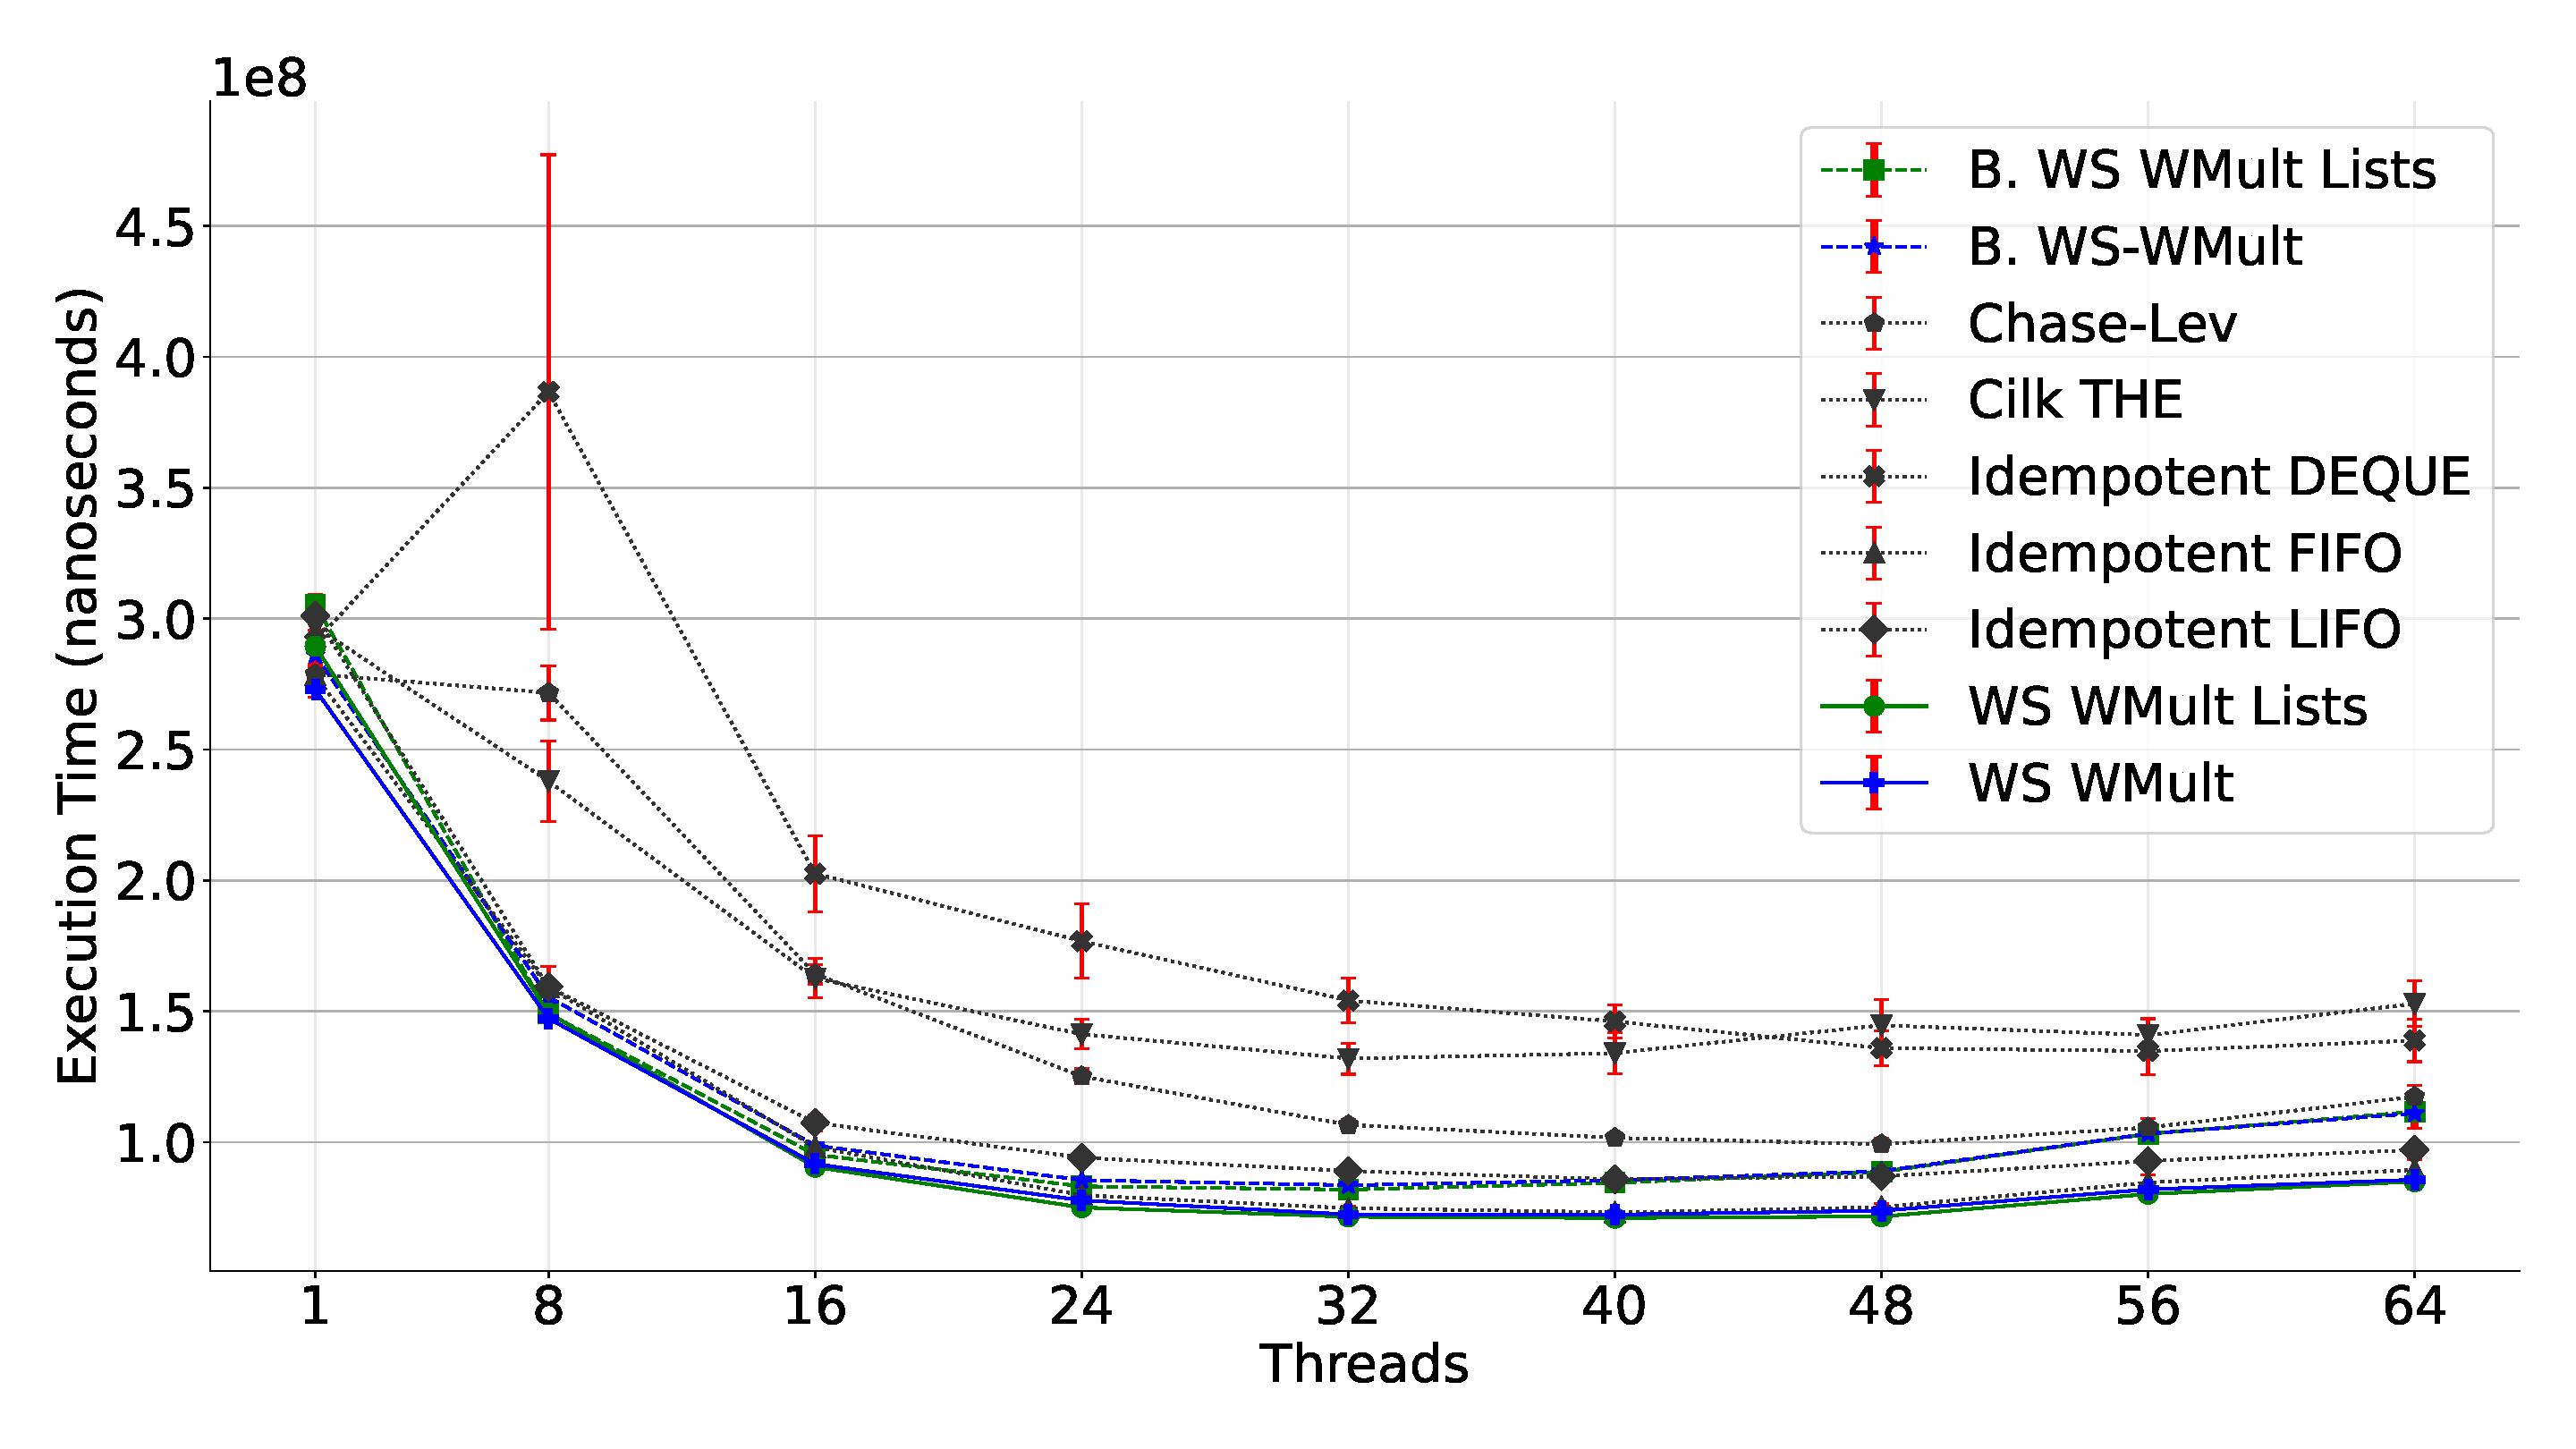
\includegraphics[width=0.48\textwidth]{contents/figures/IV_6_mean-TORUS3D-Directed-1000000.pdf}
  }

  \subfloat[\label{fig:random:256}Graph: Directed Random. Initial size of 256 entries]{
    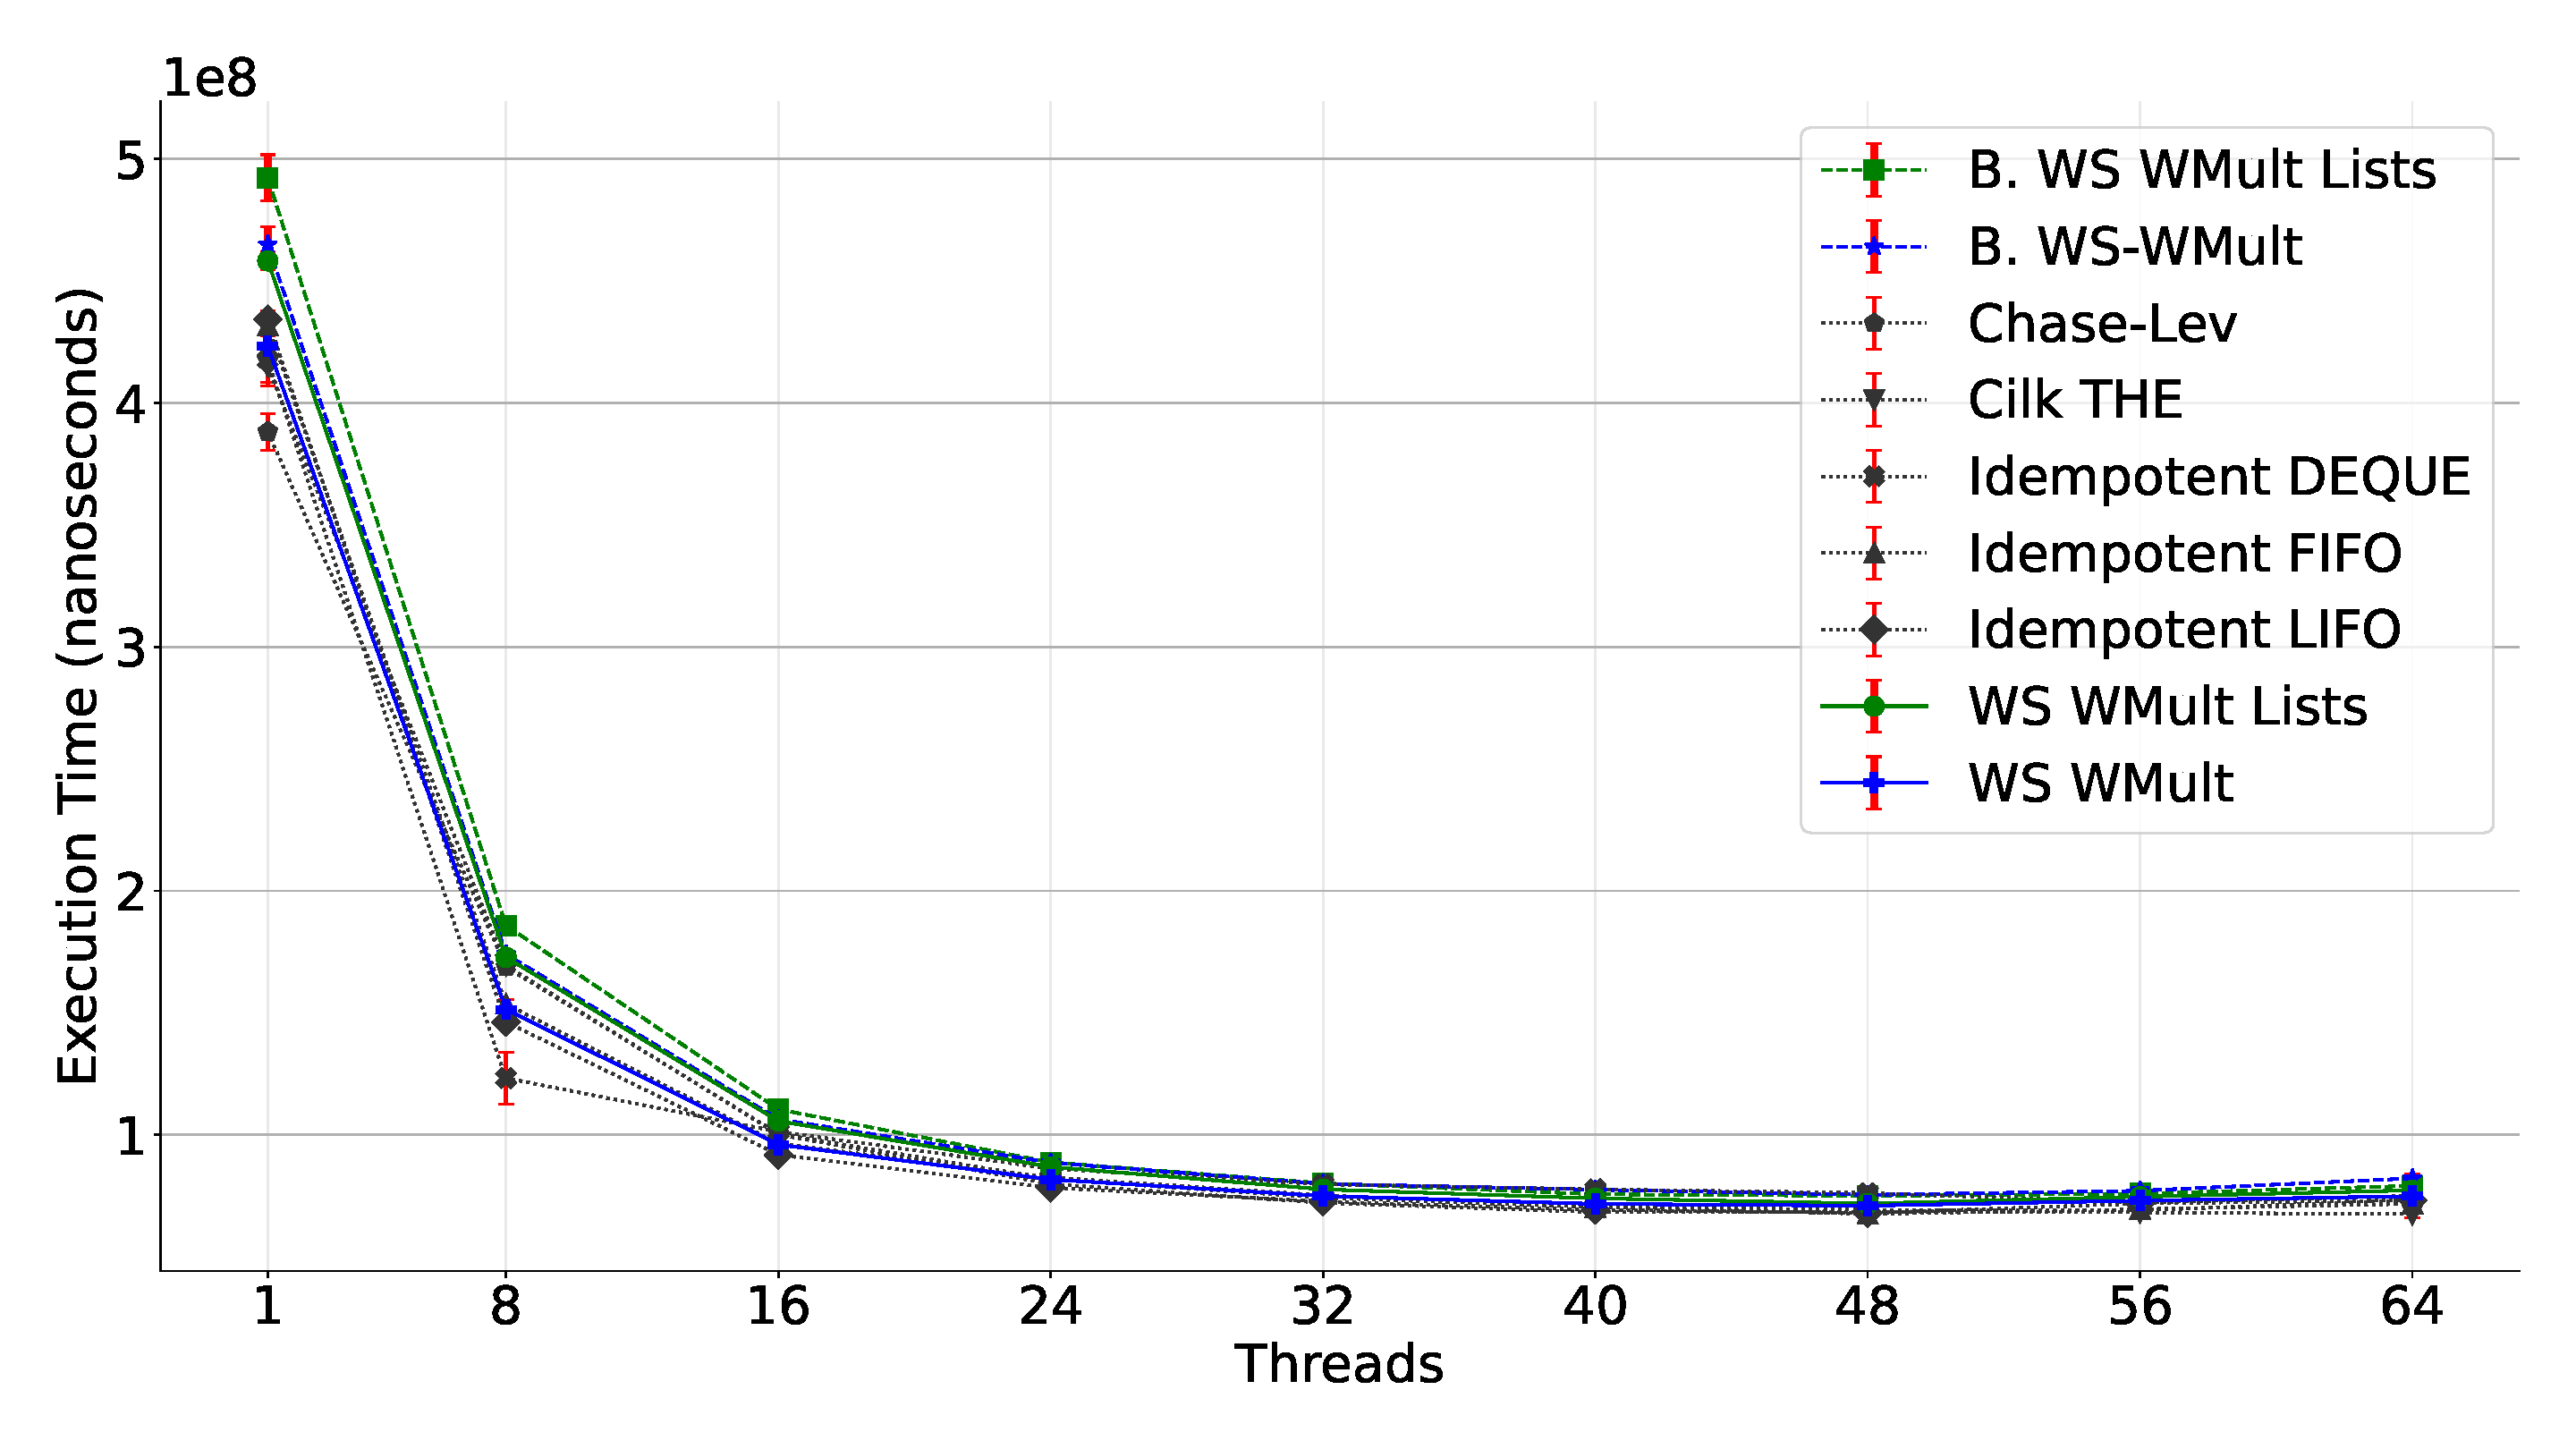
\includegraphics[width=0.48\textwidth]{contents/figures/IV_6_mean-RANDOM-Directed-256.pdf}
  }
  \subfloat[\label{fig:random:1000000}Graph: Directed Random: Initial size of 1,000,000 entries]{
    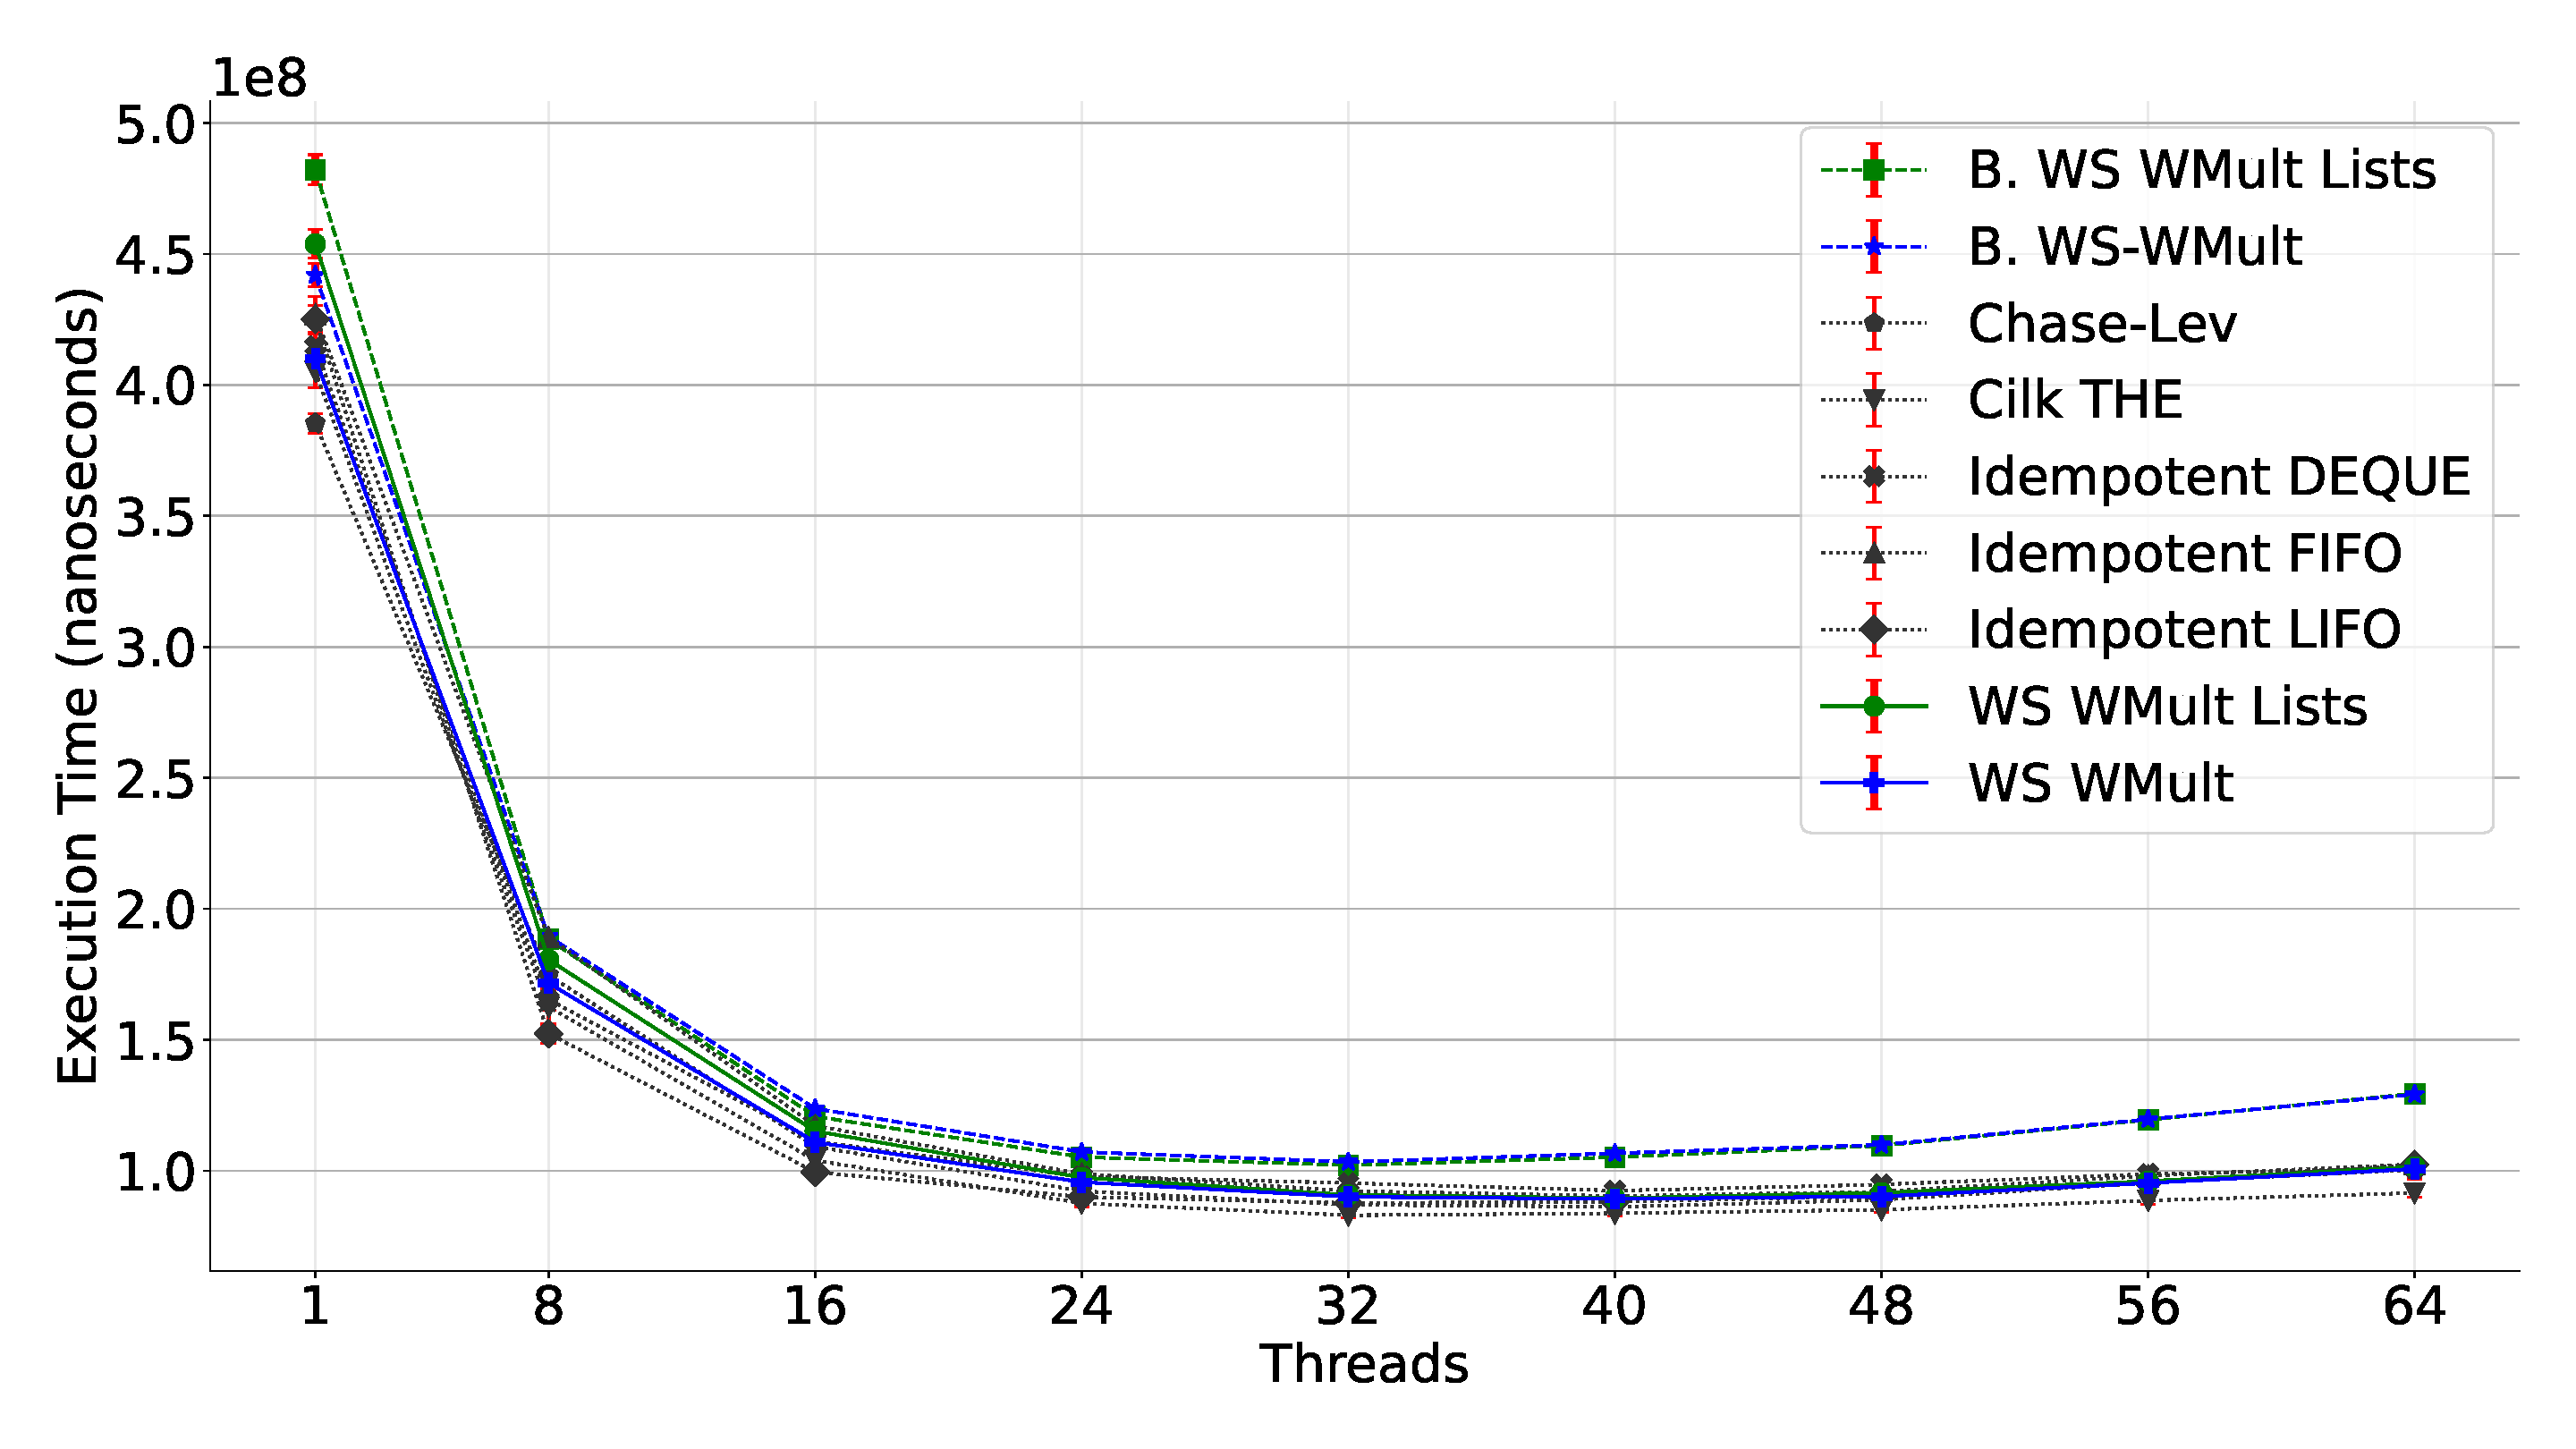
\includegraphics[width=0.48\textwidth]{contents/figures/IV_6_mean-RANDOM-Directed-1000000.pdf}
  }

  \caption{\label{fig:graphapplication} Mean times reported for executing the graph application benchmark.}
\end{figure}


Repeated work was measured indirectly through the total number of \Puts (work to be executed), which was compared to the total number of \Puts in sequential executions (i.e., $1,000,000$). The difference between these two numbers is called surplus work. Surplus work in all algorithms with FIFO insert/extract policy was generally low, less than $0.7\%$. All these algorithms implement work-stealing with relaxed semantics. Thus, even if all surplus work was due to relaxation (recall that surplus work can occur even with non-relaxed work-stealing algorithms), it rarely happened, with little impact on performance. In sharp contrast, in all algorithms where the owner follows the LIFO insert/extract policy (Cilk THE, Chase-Lev, idempotent LIFO, and idempotent Deque), surplus work ranged between \(1\%\) and \(56\%\). Therefore, neither multiplicity nor idempotency per se increased surplus work considerably, and the dominant factor seems to be the task insert/extract policy combined with the solved problem. Figure~\ref{fig:surplusgraphapplication} depicts the surplus work of the experiments in Figure~\ref{fig:graphapplication}.

In all algorithms, not all tasks are executed. Processes are constantly checking the distinct number of vertices that have been processed so far, and when this number reaches $1,000,000$, the spanning tree is completed, and the experiment terminates. It can be the case that some vertices remain in one or more work-stealing structures when the tree is finished; not all surplus work is executed. We measured the executed surplus work, i.e., the difference between the total number of \Takes (actual work executed) and the total number of \Takes in sequential executions (i.e., $1,000,000$). Executed surplus work in Cilk THE, Chase-Lev, idempotent LIFO, and idempotent Deque ranged between \(1\%\) and \(49\%\). Figure~\ref{fig:exec-surplusgraphapplication} shows the executed surplus work of the experiments in Figure~\ref{fig:graphapplication}. Finally, in some experiments (e.g., Random graphs), \NCWSM executed more surplus work than the algorithms with LIFO insert/extract policy, but still, it performed slightly better. We attribute this to the fact that in the FIFO policy, \Takes are more likely to read tasks from cache memory, whereas in LIFO, \Takes are more likely to read from main memory, which is costly. Appendix \ref{sec:results-irreg-graph} contains all results of the benchmark.



\begin{figure}
  \subfloat[\label{fig:surplustorus2ddirected:256}Surplus work: Directed Torus 2D. Initial size of 256 items.]{
    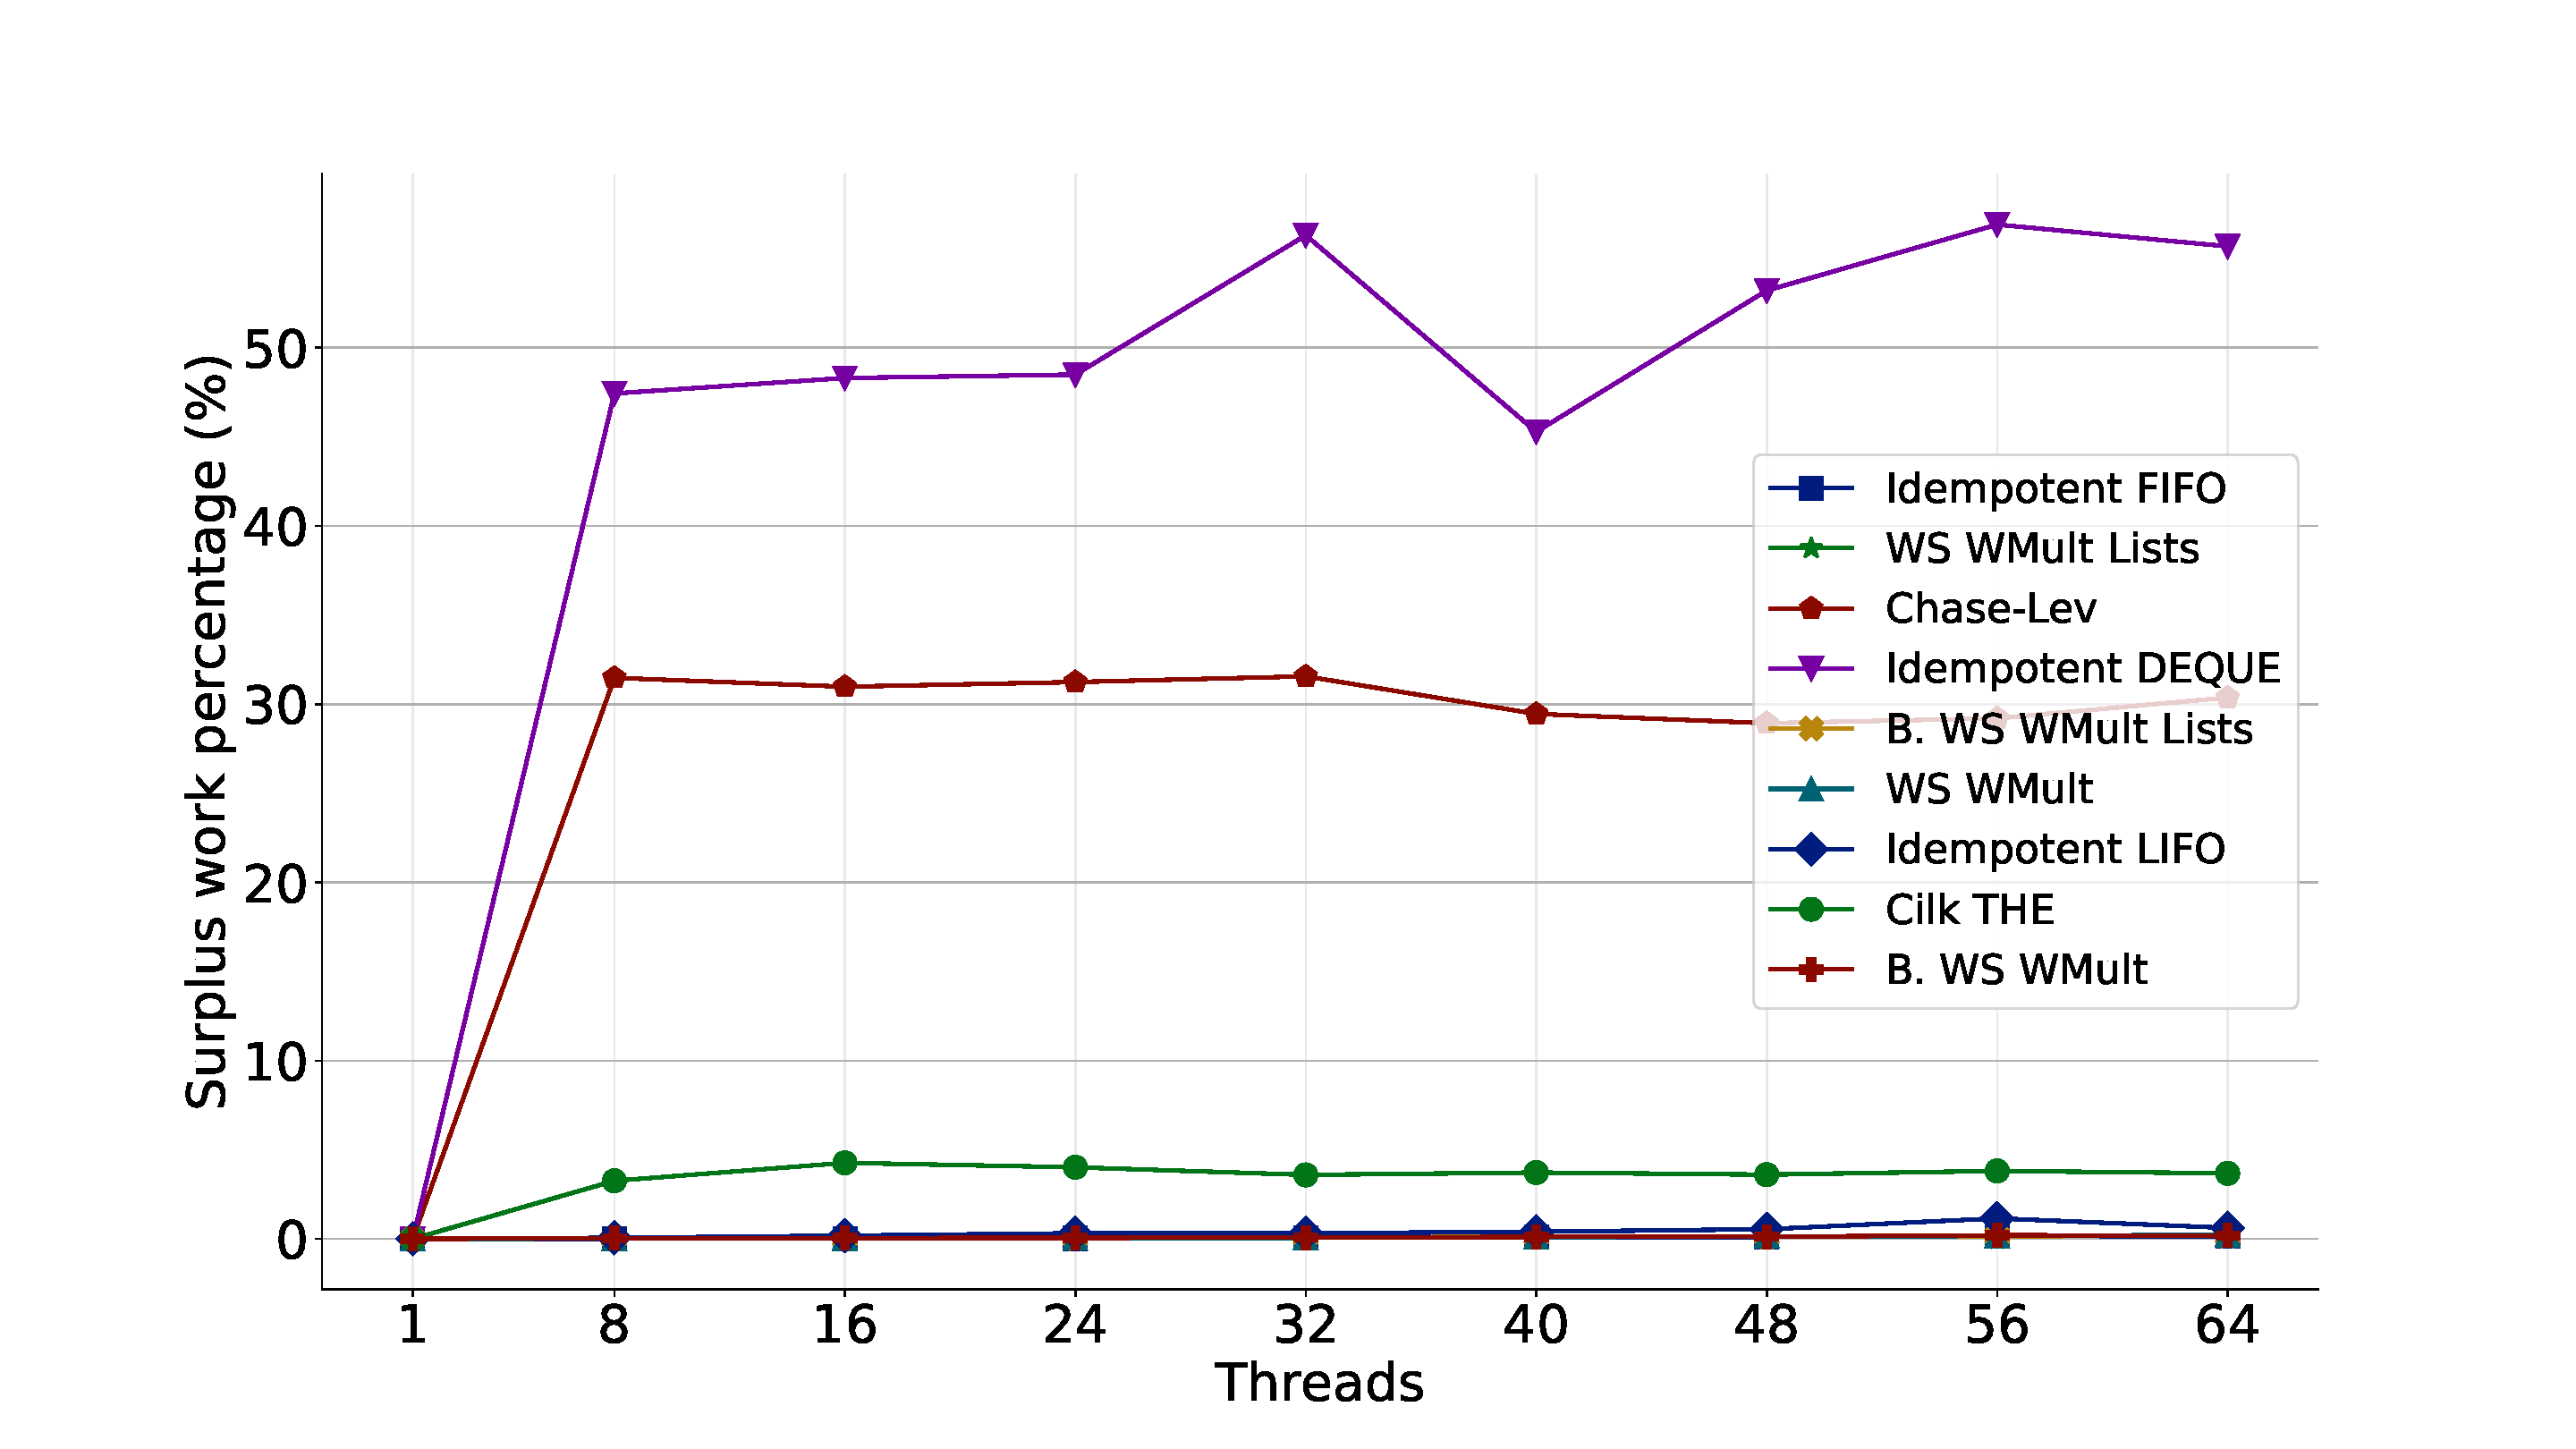
\includegraphics[width=0.48\textwidth]{contents/figures/IV_6_mult-torus_2d_directed_256.pdf}
  }
  \subfloat[\label{fig:surplustorus2ddirected:1000000}Surplus work: Directed Torus 2D. Initial size of 1,000,000 items.]{
    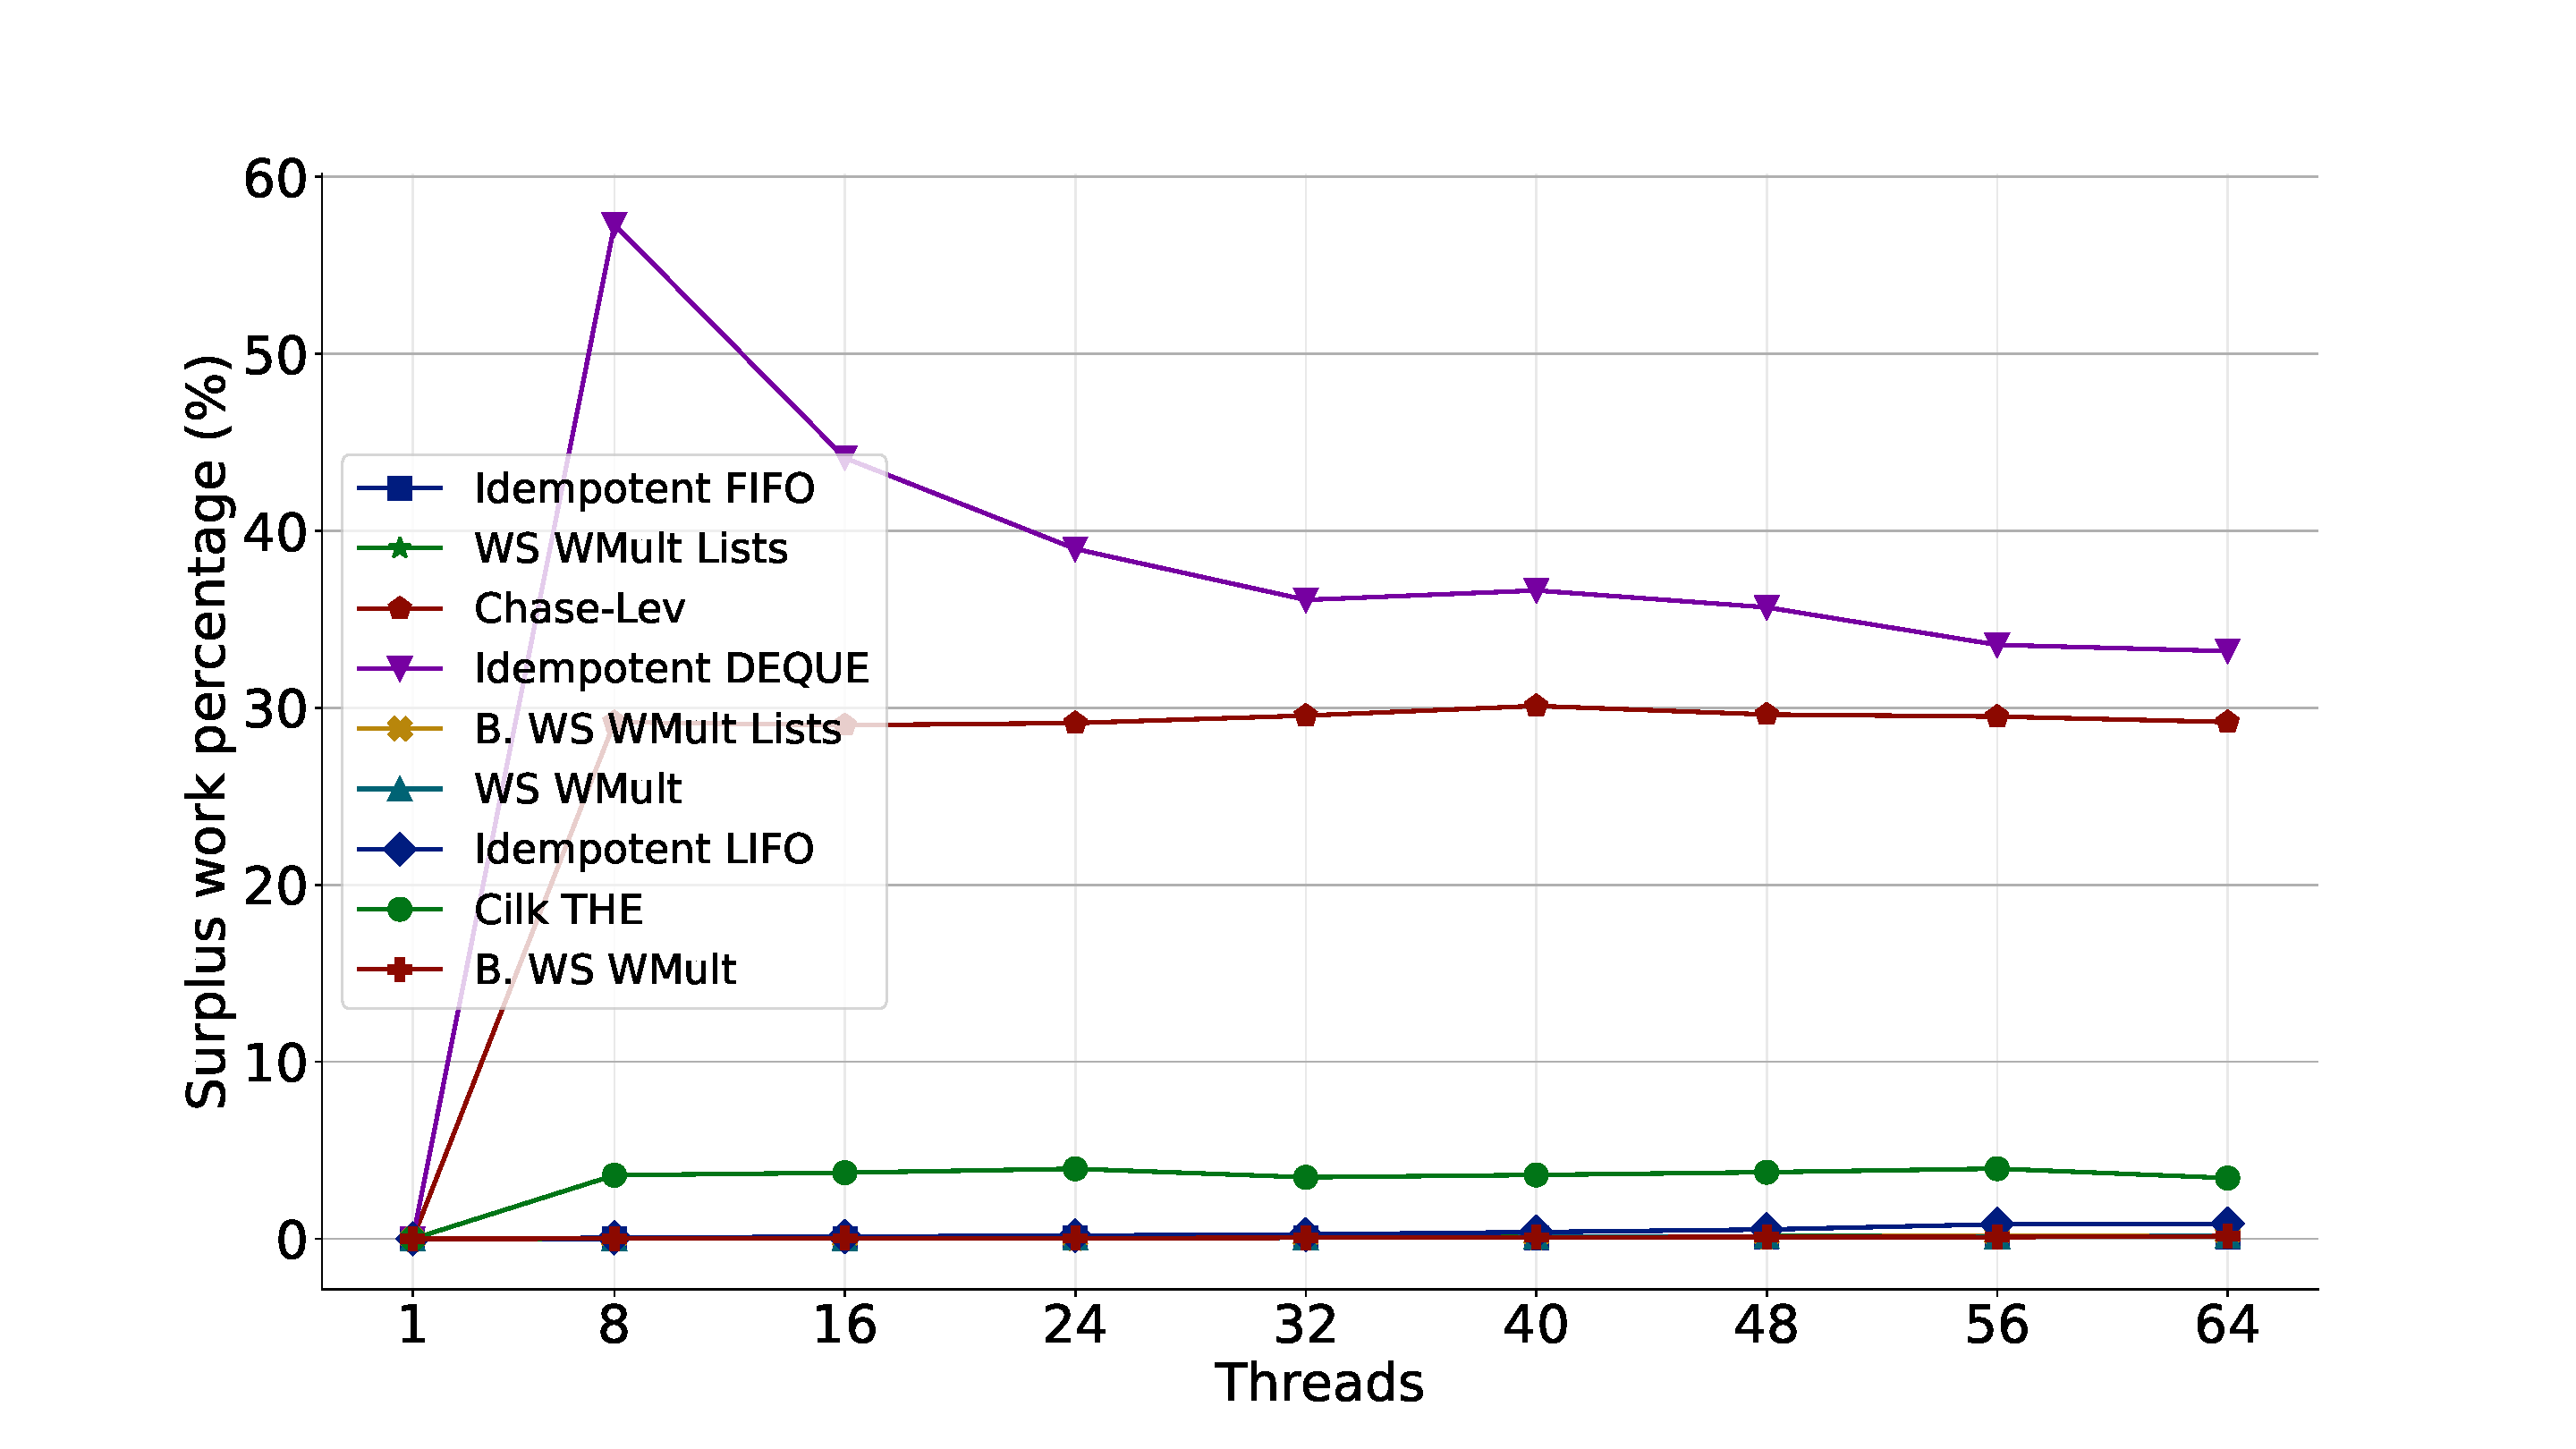
\includegraphics[width=0.48\textwidth]{contents/figures/IV_6_mult-torus_2d_directed_1m.pdf}
  }

  \subfloat[\label{fig:surplustorus3ddirected:256}Surplus work: Directed Torus 3D. Initial size of 256 items.]{
    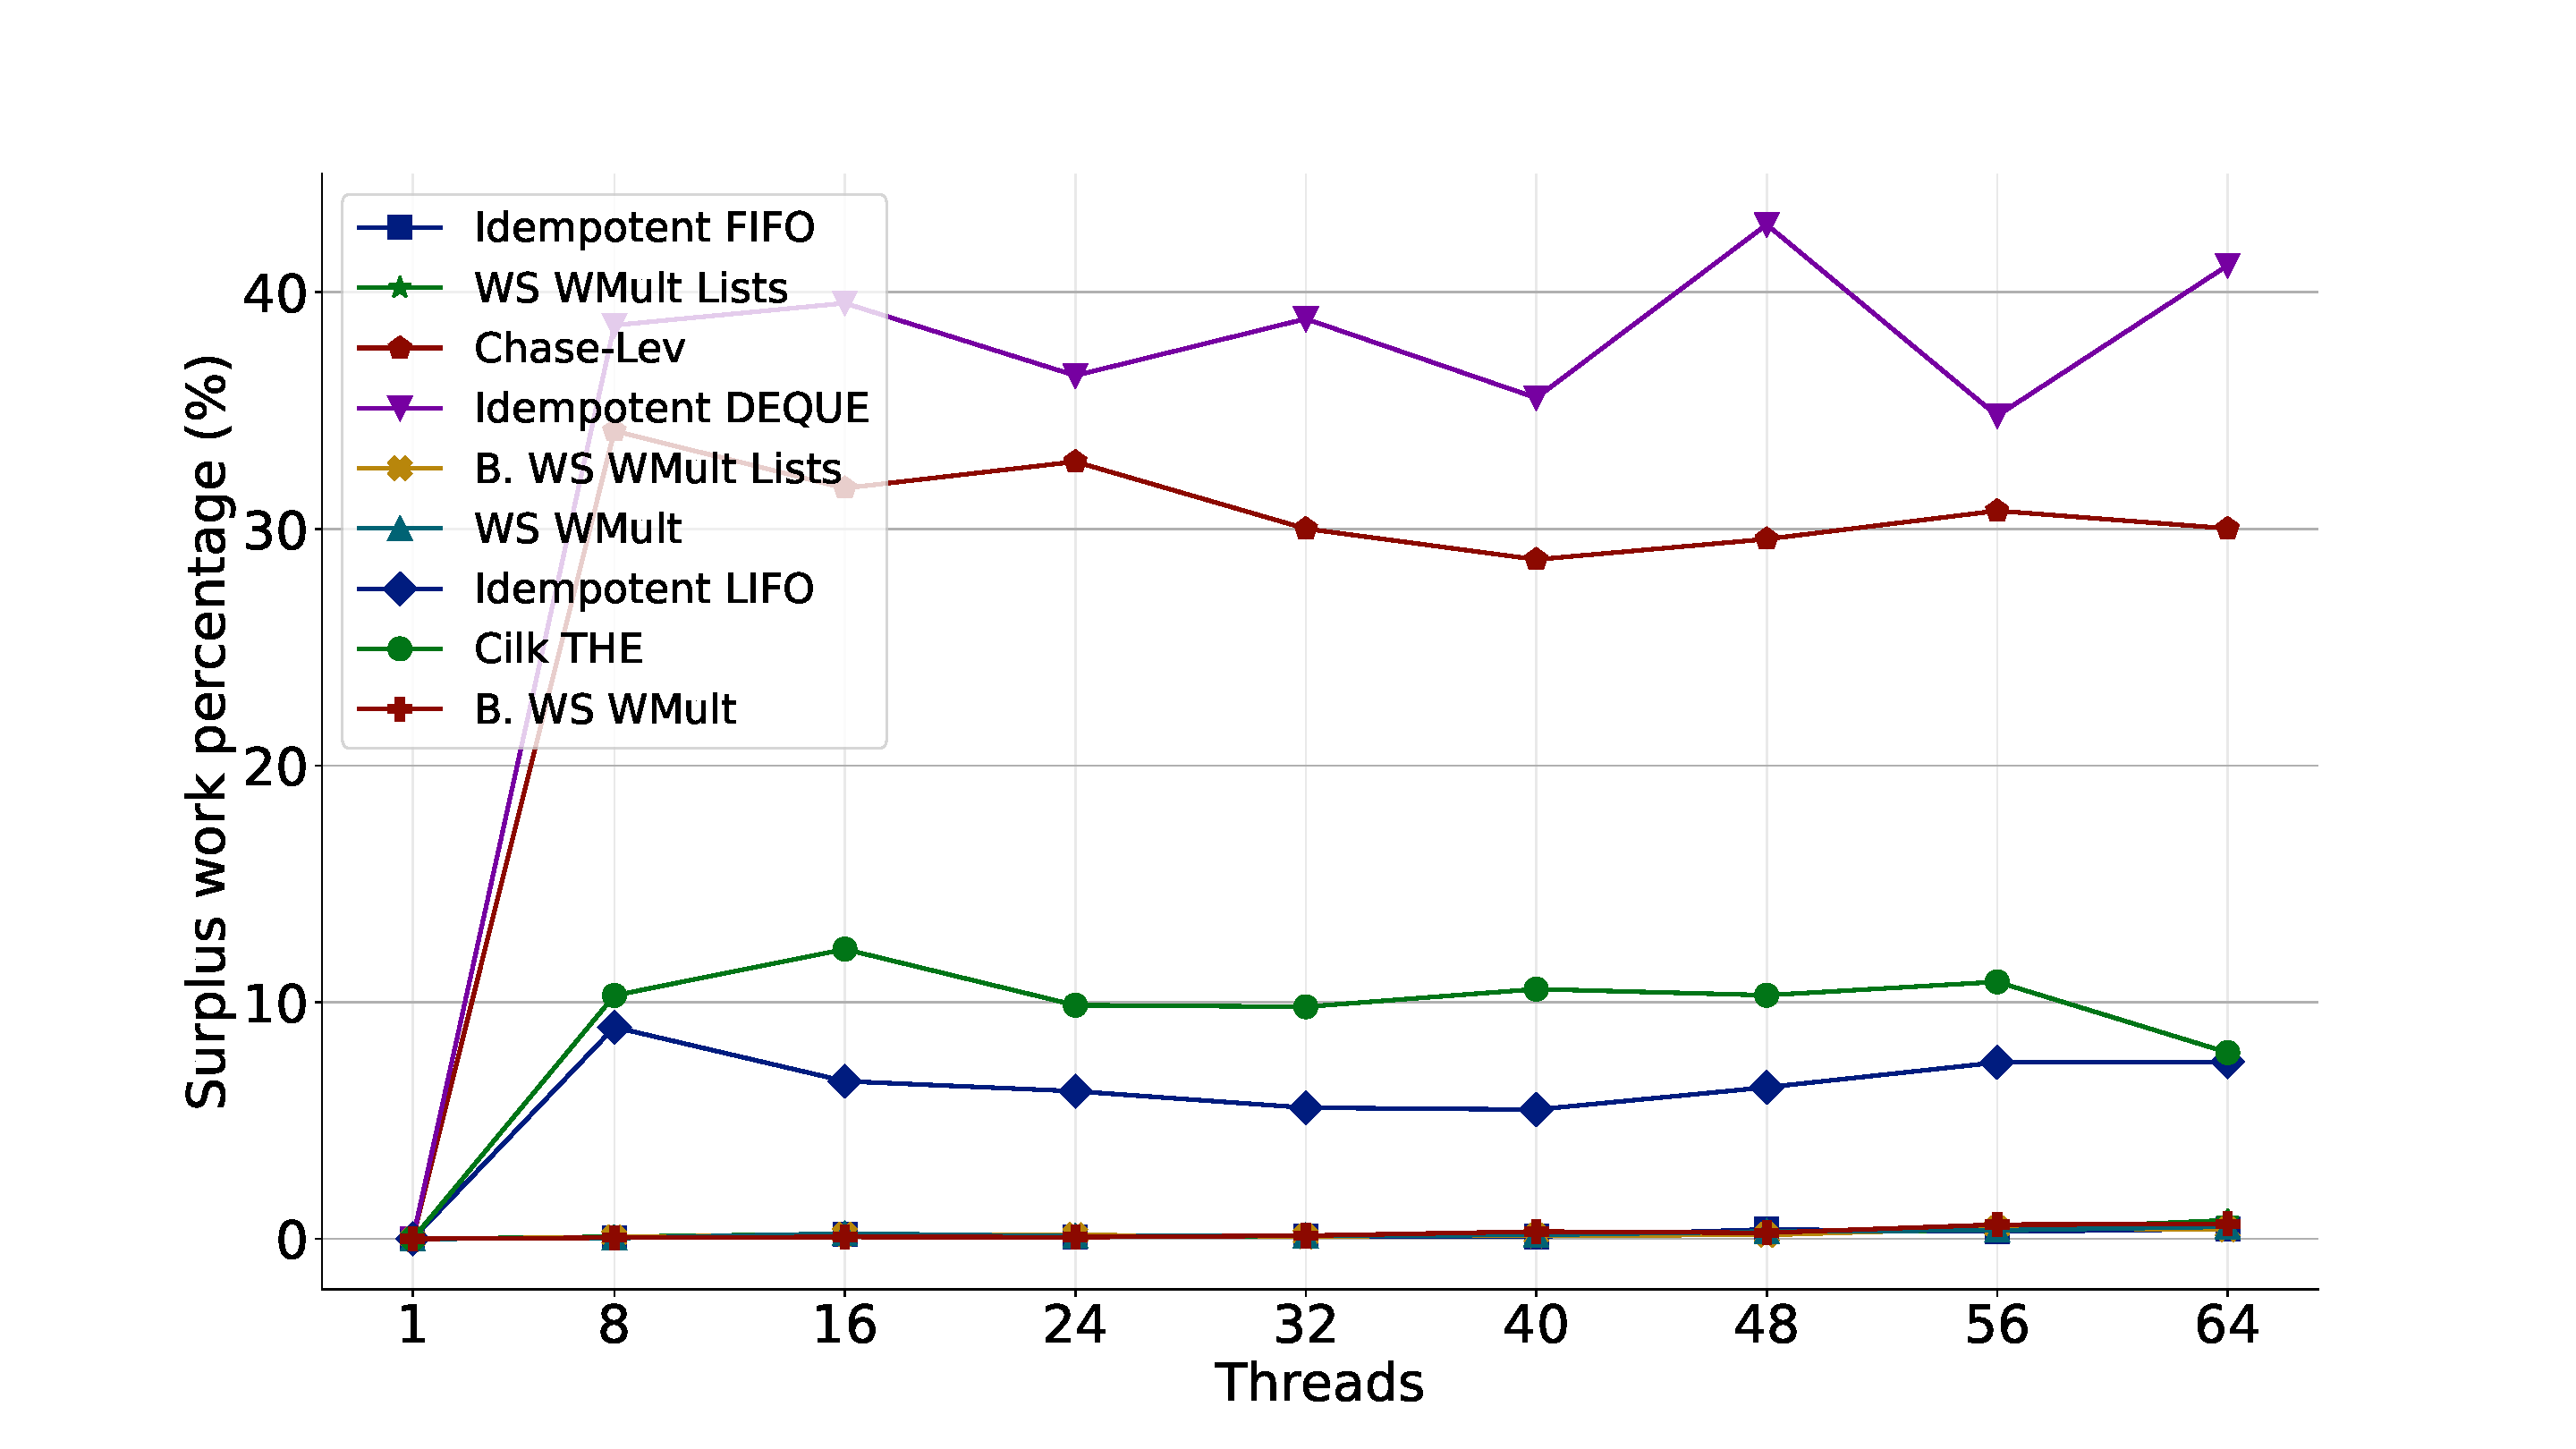
\includegraphics[width=0.48\textwidth]{contents/figures/IV_6_mult-torus_3d_directed_256.pdf}
  }
  \subfloat[\label{fig:surplustorus3ddirected:1000000}Surplus work: Directed Torus 3D. Initial size of 1,000,000 items.]{
    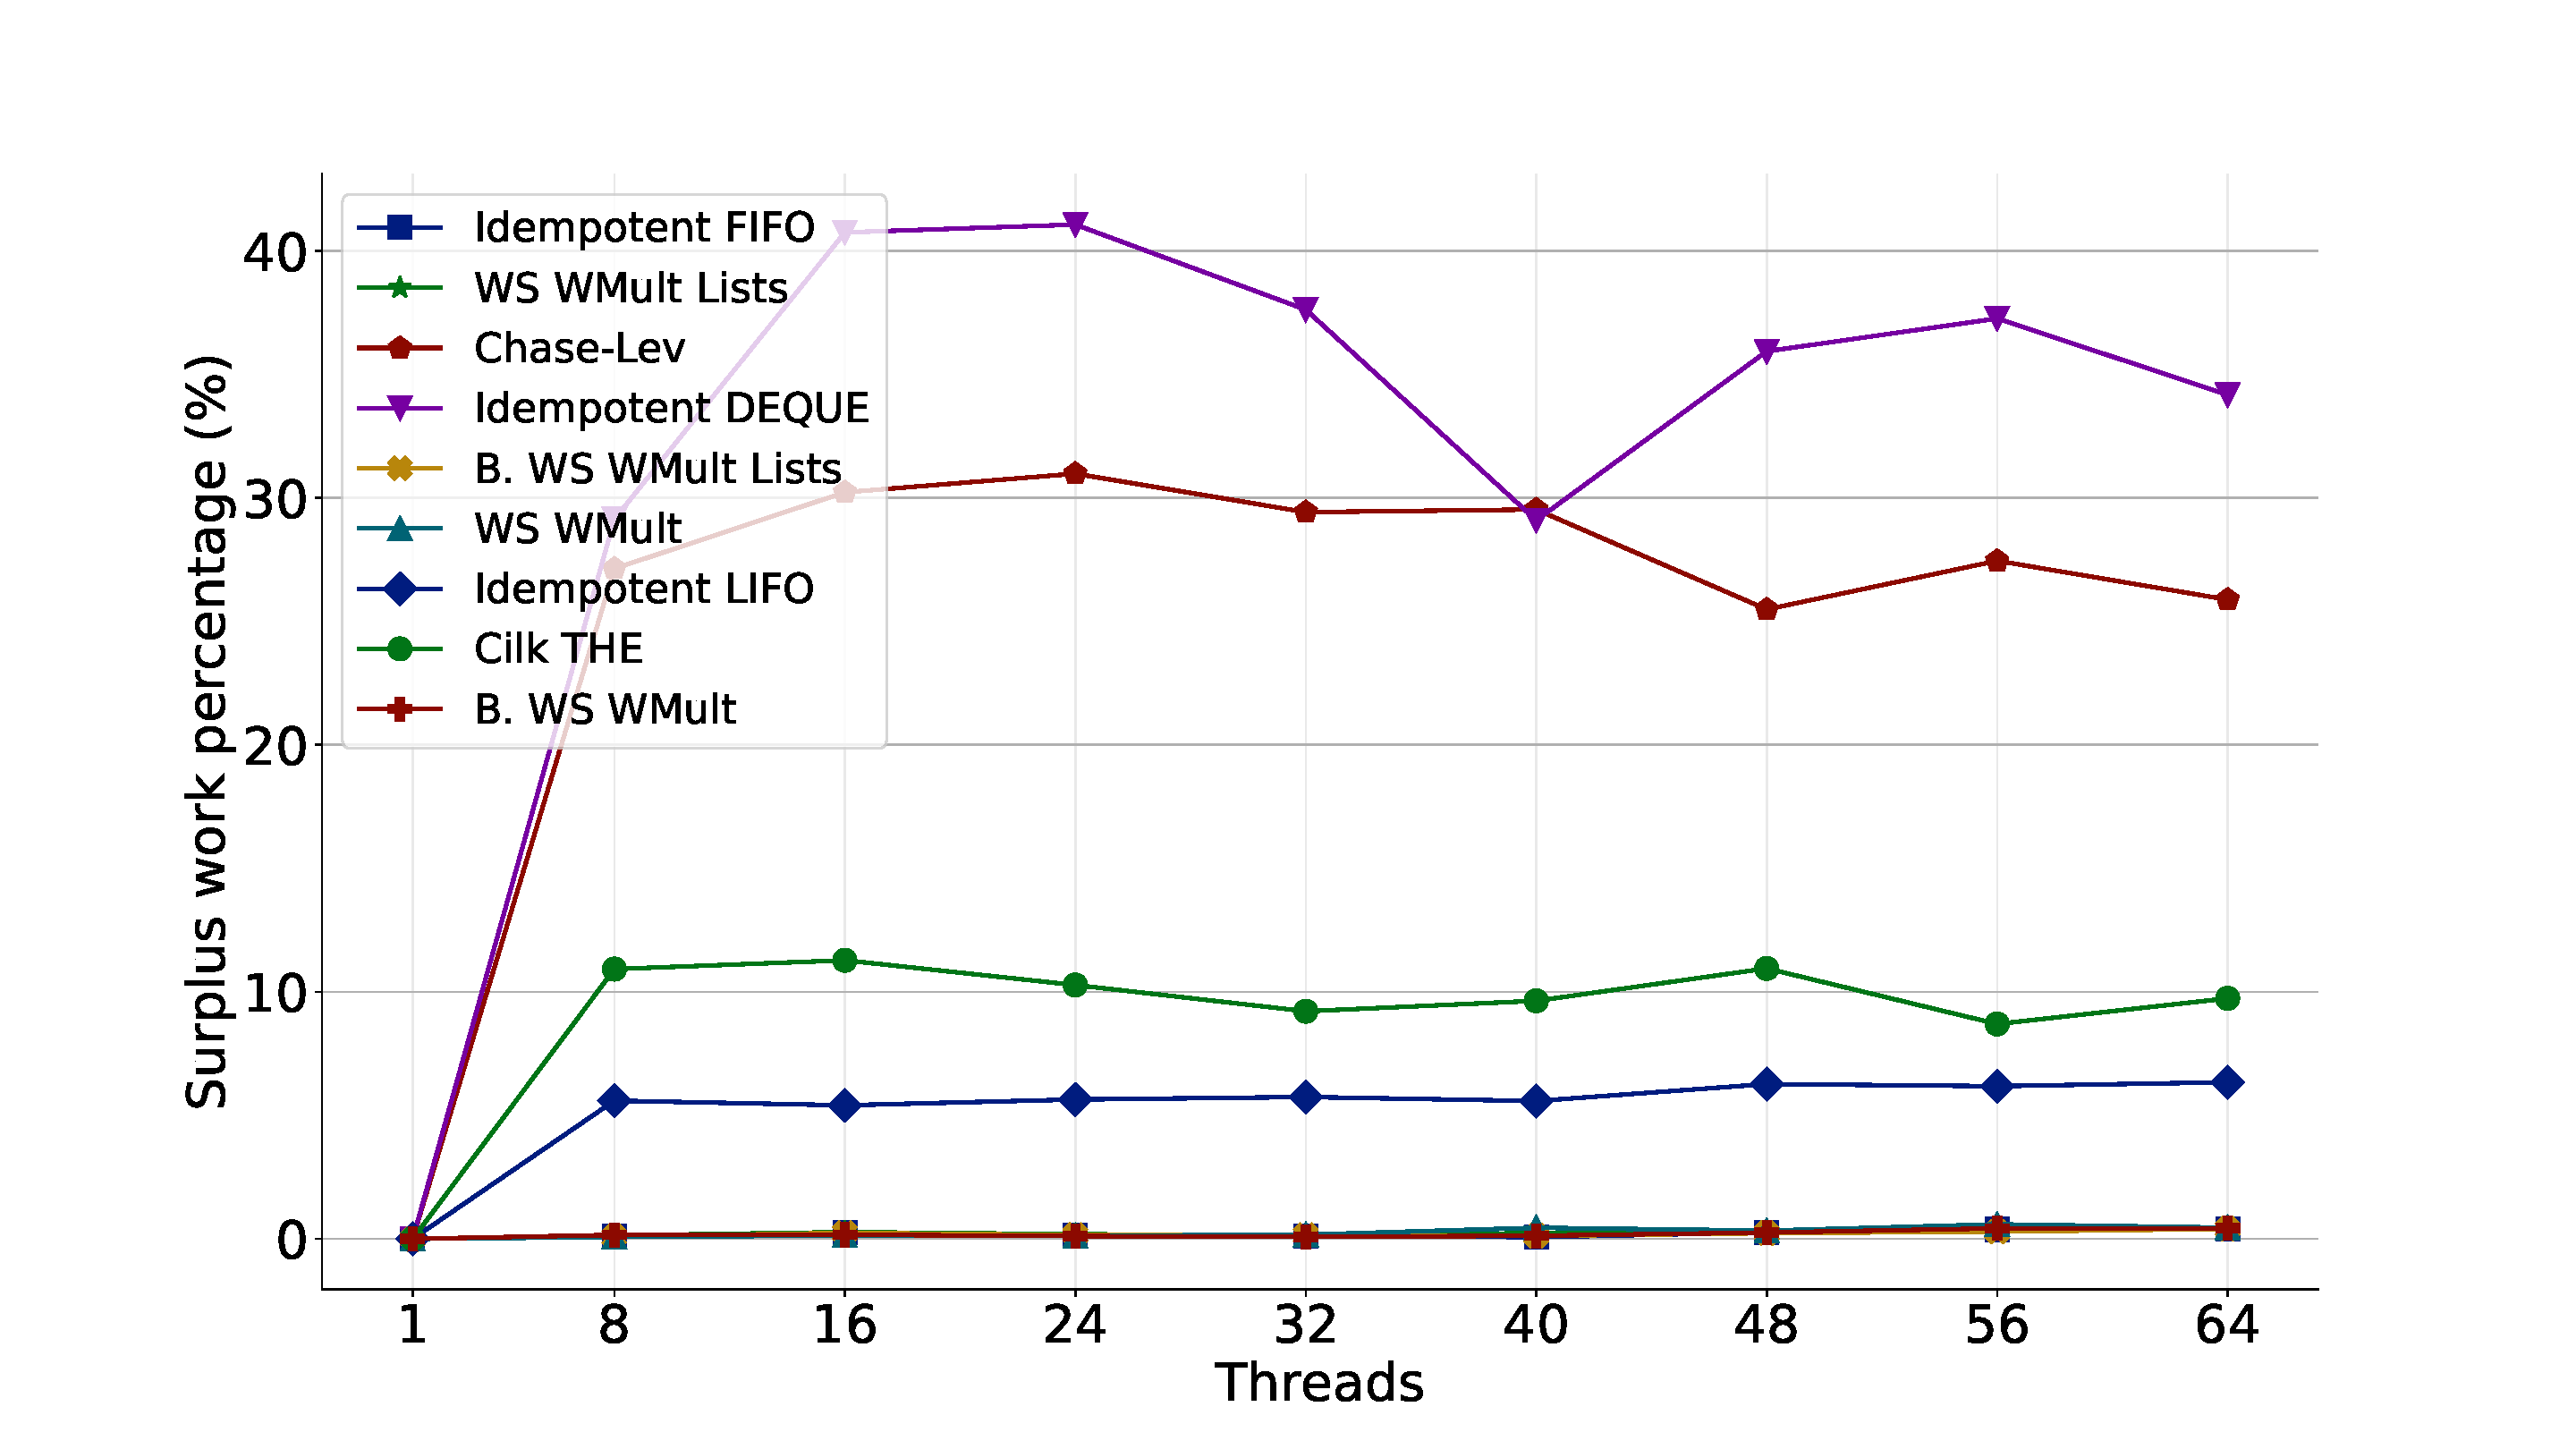
\includegraphics[width=0.48\textwidth]{contents/figures/IV_6_mult-torus_3d_directed_1m.pdf}
  }

  \subfloat[\label{fig:surplusrandom:256}Surplus work: Directed Random. Initial size of 256 items.]{
    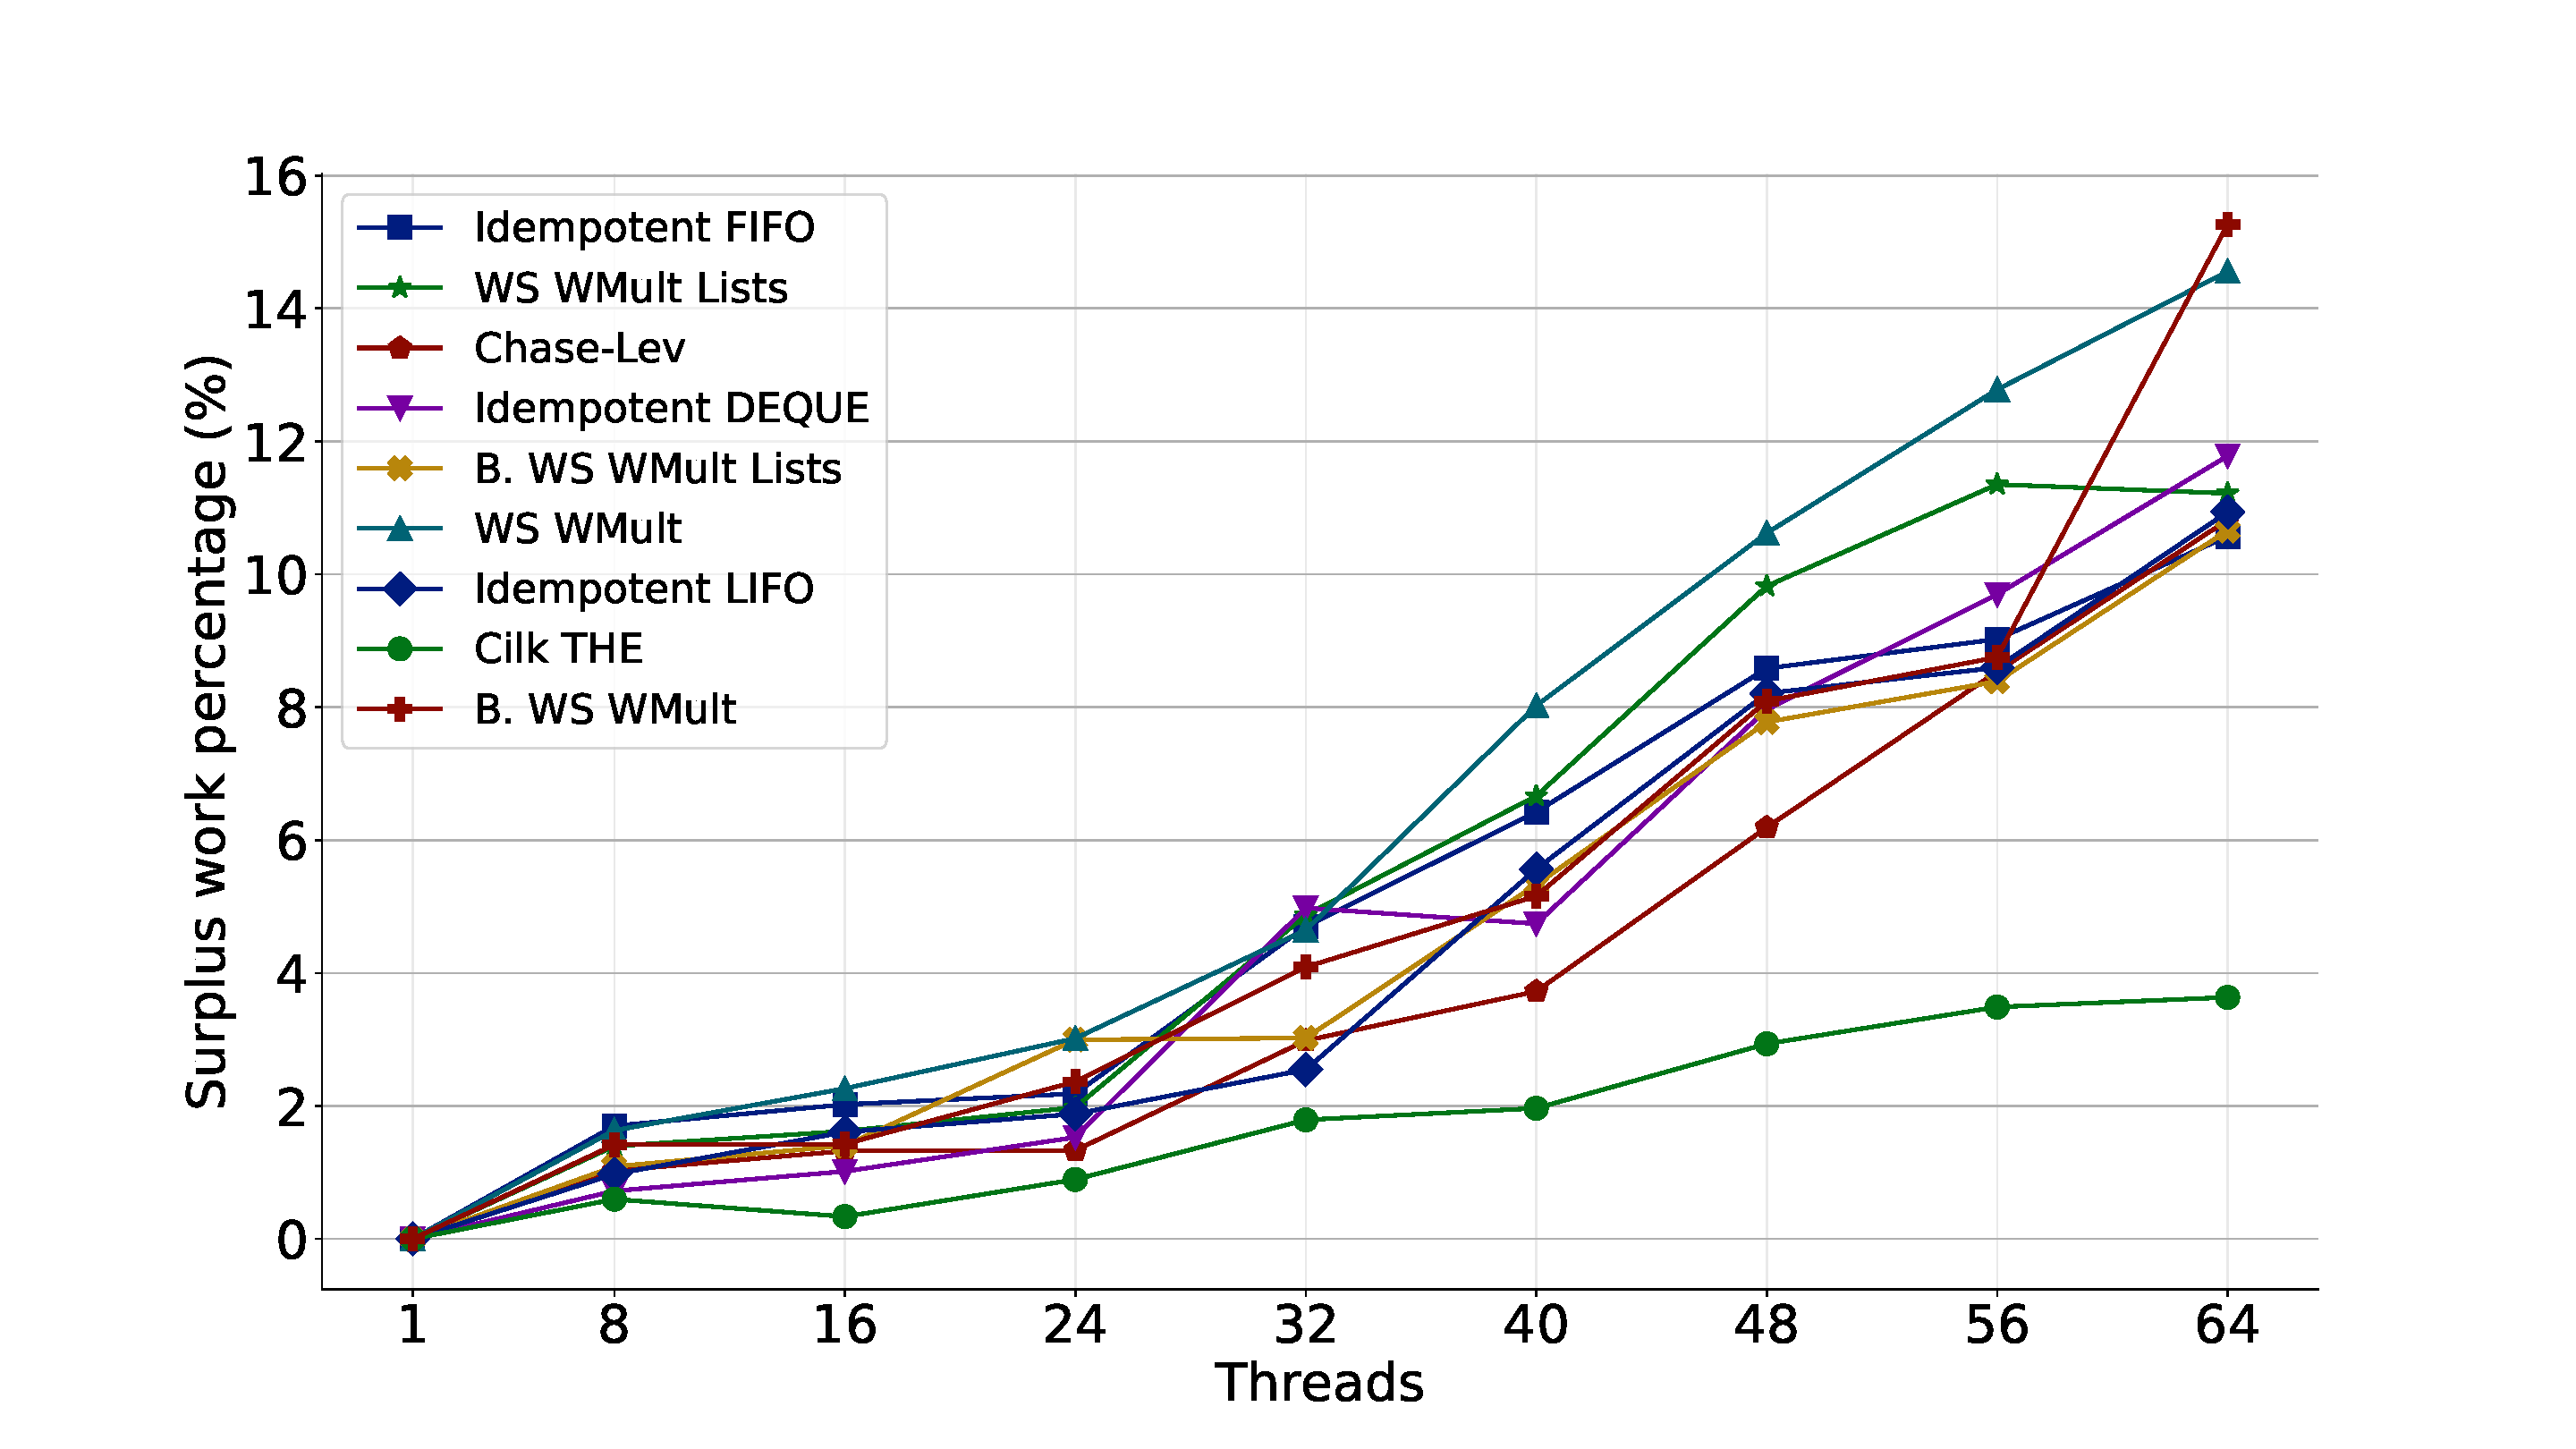
\includegraphics[width=0.48\textwidth]{contents/figures/IV_6_mult-random_directed_256.pdf}
  }
  \subfloat[\label{fig:surplusrandom:1000000}Surplus work: Directed Random: Initial size of 1,000,000 items.]{
    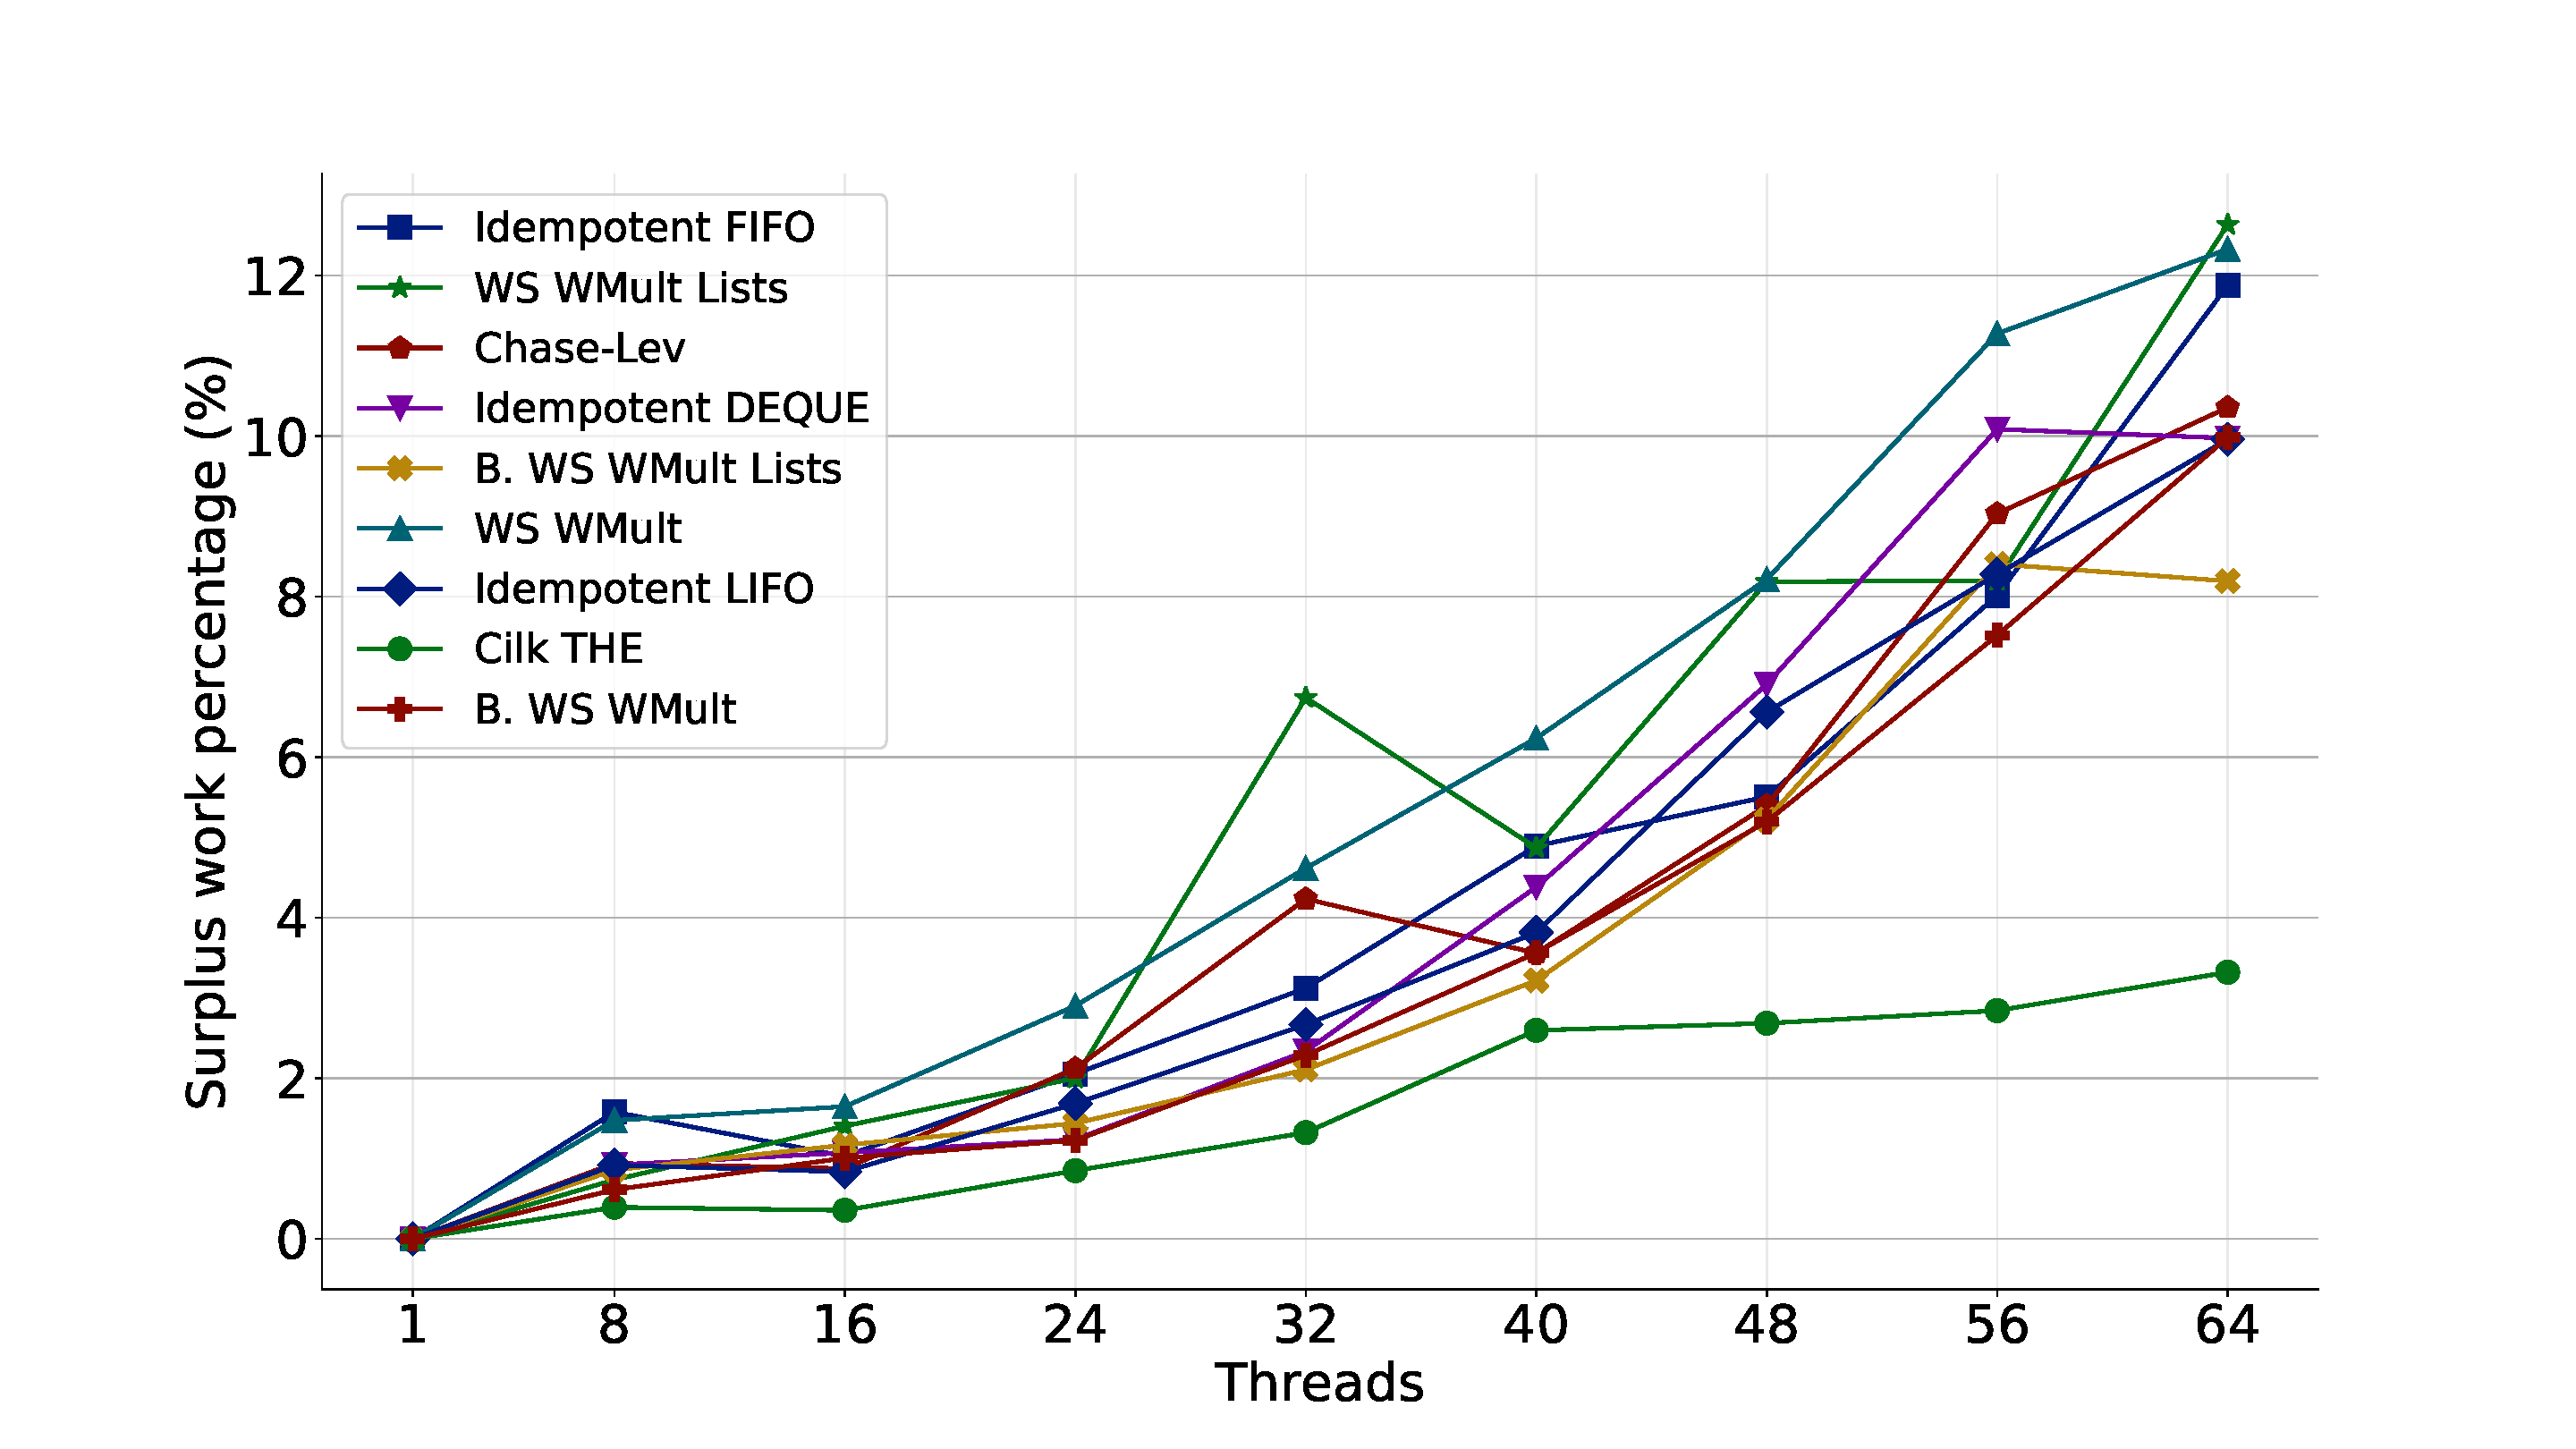
\includegraphics[width=0.48\textwidth]{contents/figures/IV_6_mult-random_directed_1m.pdf}
  }

  \caption{\label{fig:surplusgraphapplication} Surplus work (percentage) of the experiments.  Surplus work: the difference between the total number of \Puts and the number of puts in sequential executions (i.e., $1,000,000$).}
\end{figure}

\begin{figure}[!ht]
  \subfloat[\label{fig:exec-surplustorus2ddirected:256}Executed surplus work: Directed Torus 2D. Initial size of 256 items.]{
    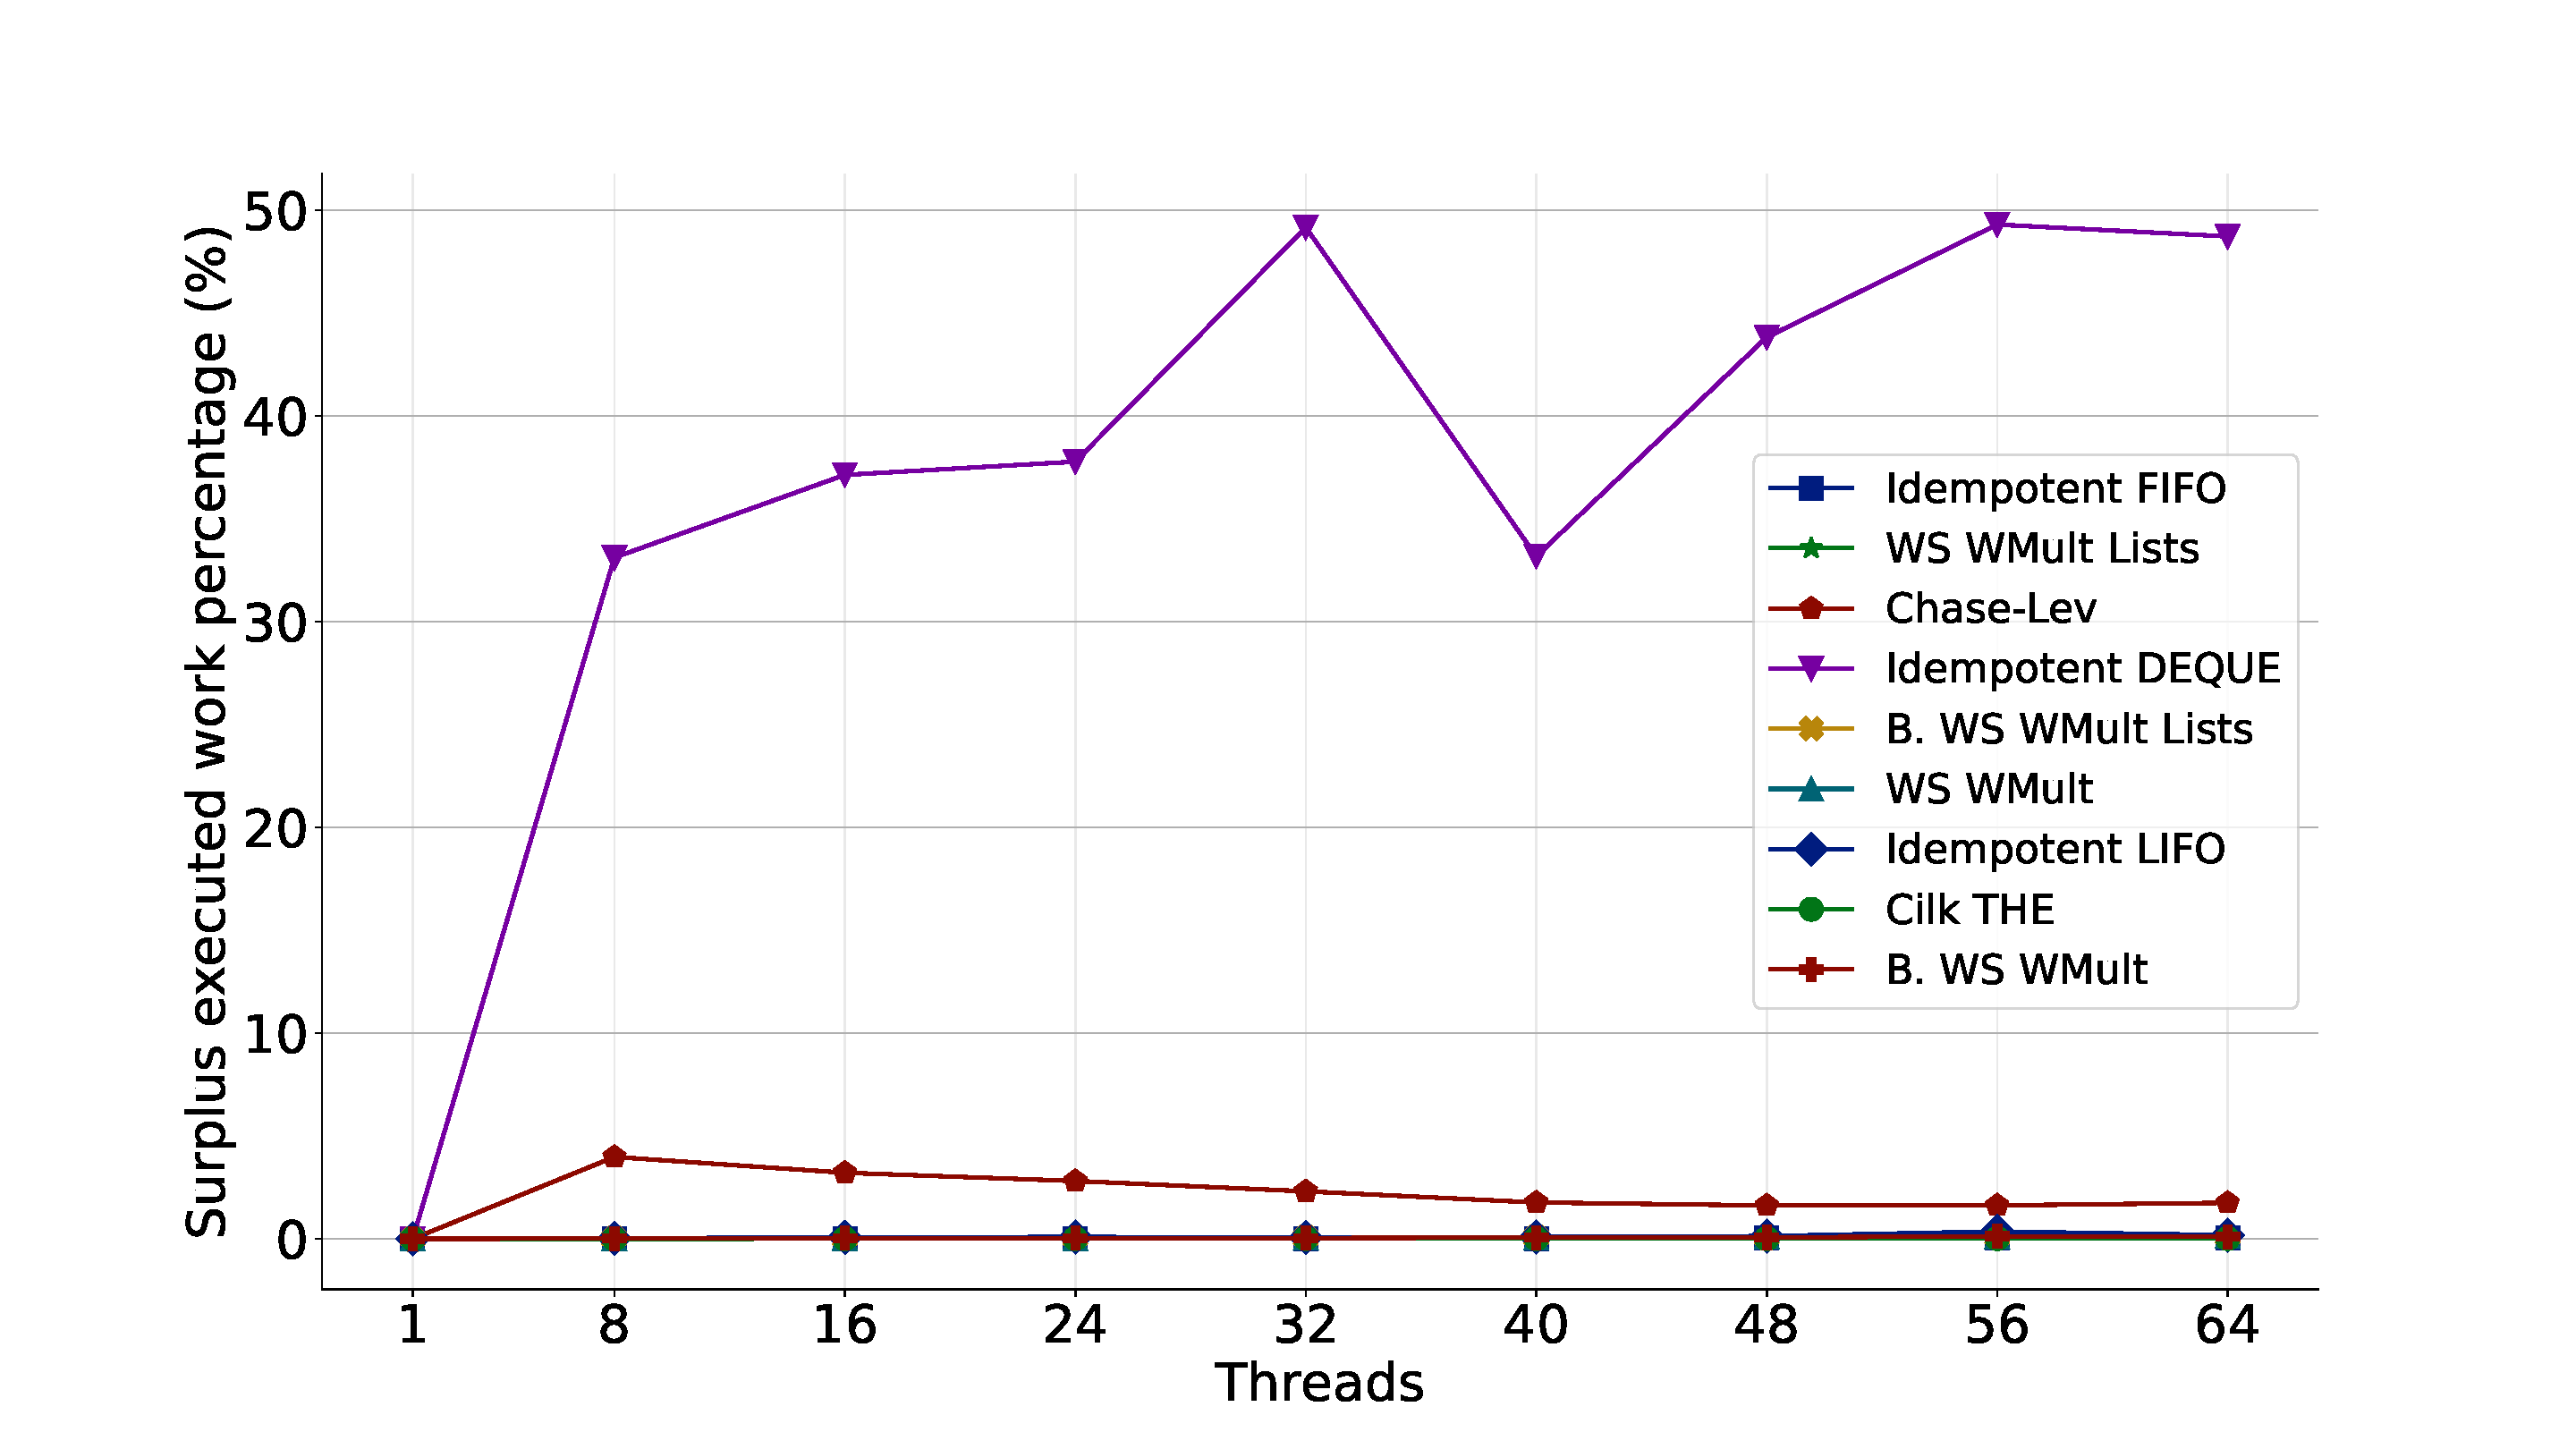
\includegraphics[width=0.48\textwidth]{contents/figures/IV_6_mult-exec-torus_2d_directed_256.pdf}
  }
  \subfloat[\label{fig:exec-surplustorus2ddirected:1000000}Executed surplus work: Directed Torus 2D. Initial size of 1,000,000 items.]{
    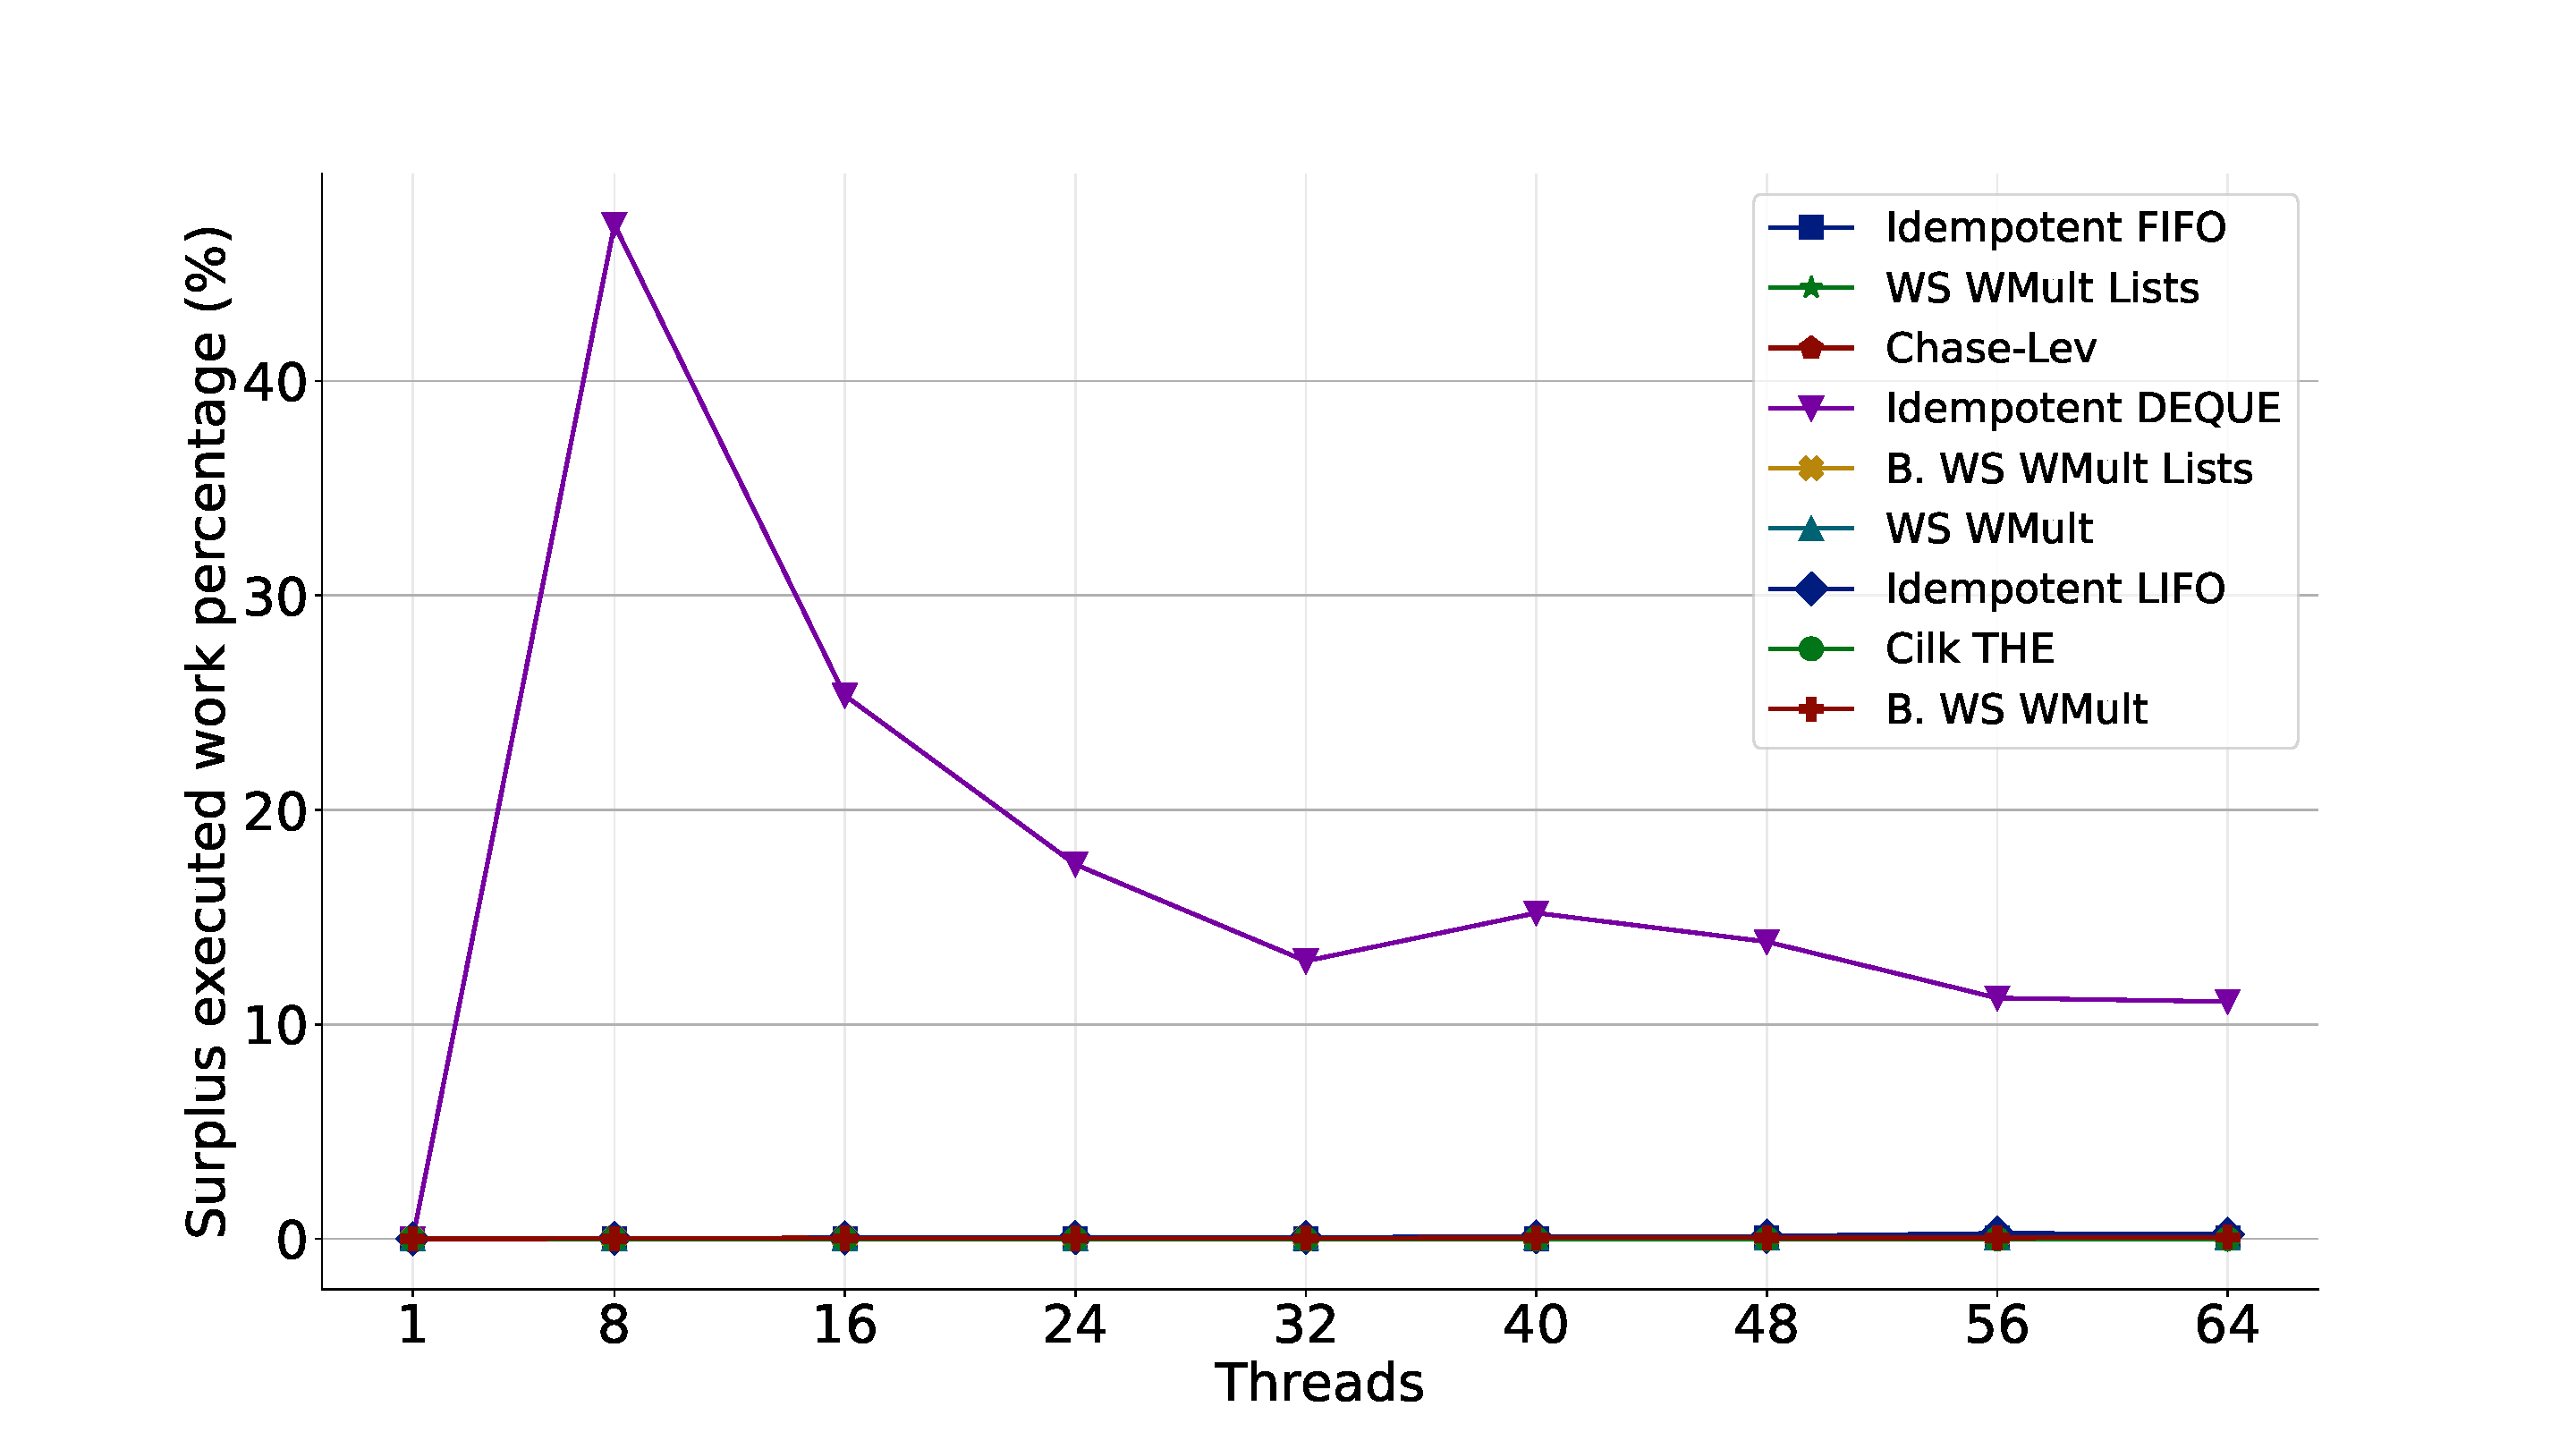
\includegraphics[width=0.48\textwidth]{contents/figures/IV_6_mult-exec-torus_2d_directed_1m.pdf}
  }

  \subfloat[\label{fig:exec-surplustorus3ddirected:256}Executed surplus work: Directed Torus 3D. Initial size of 256 items.]{
    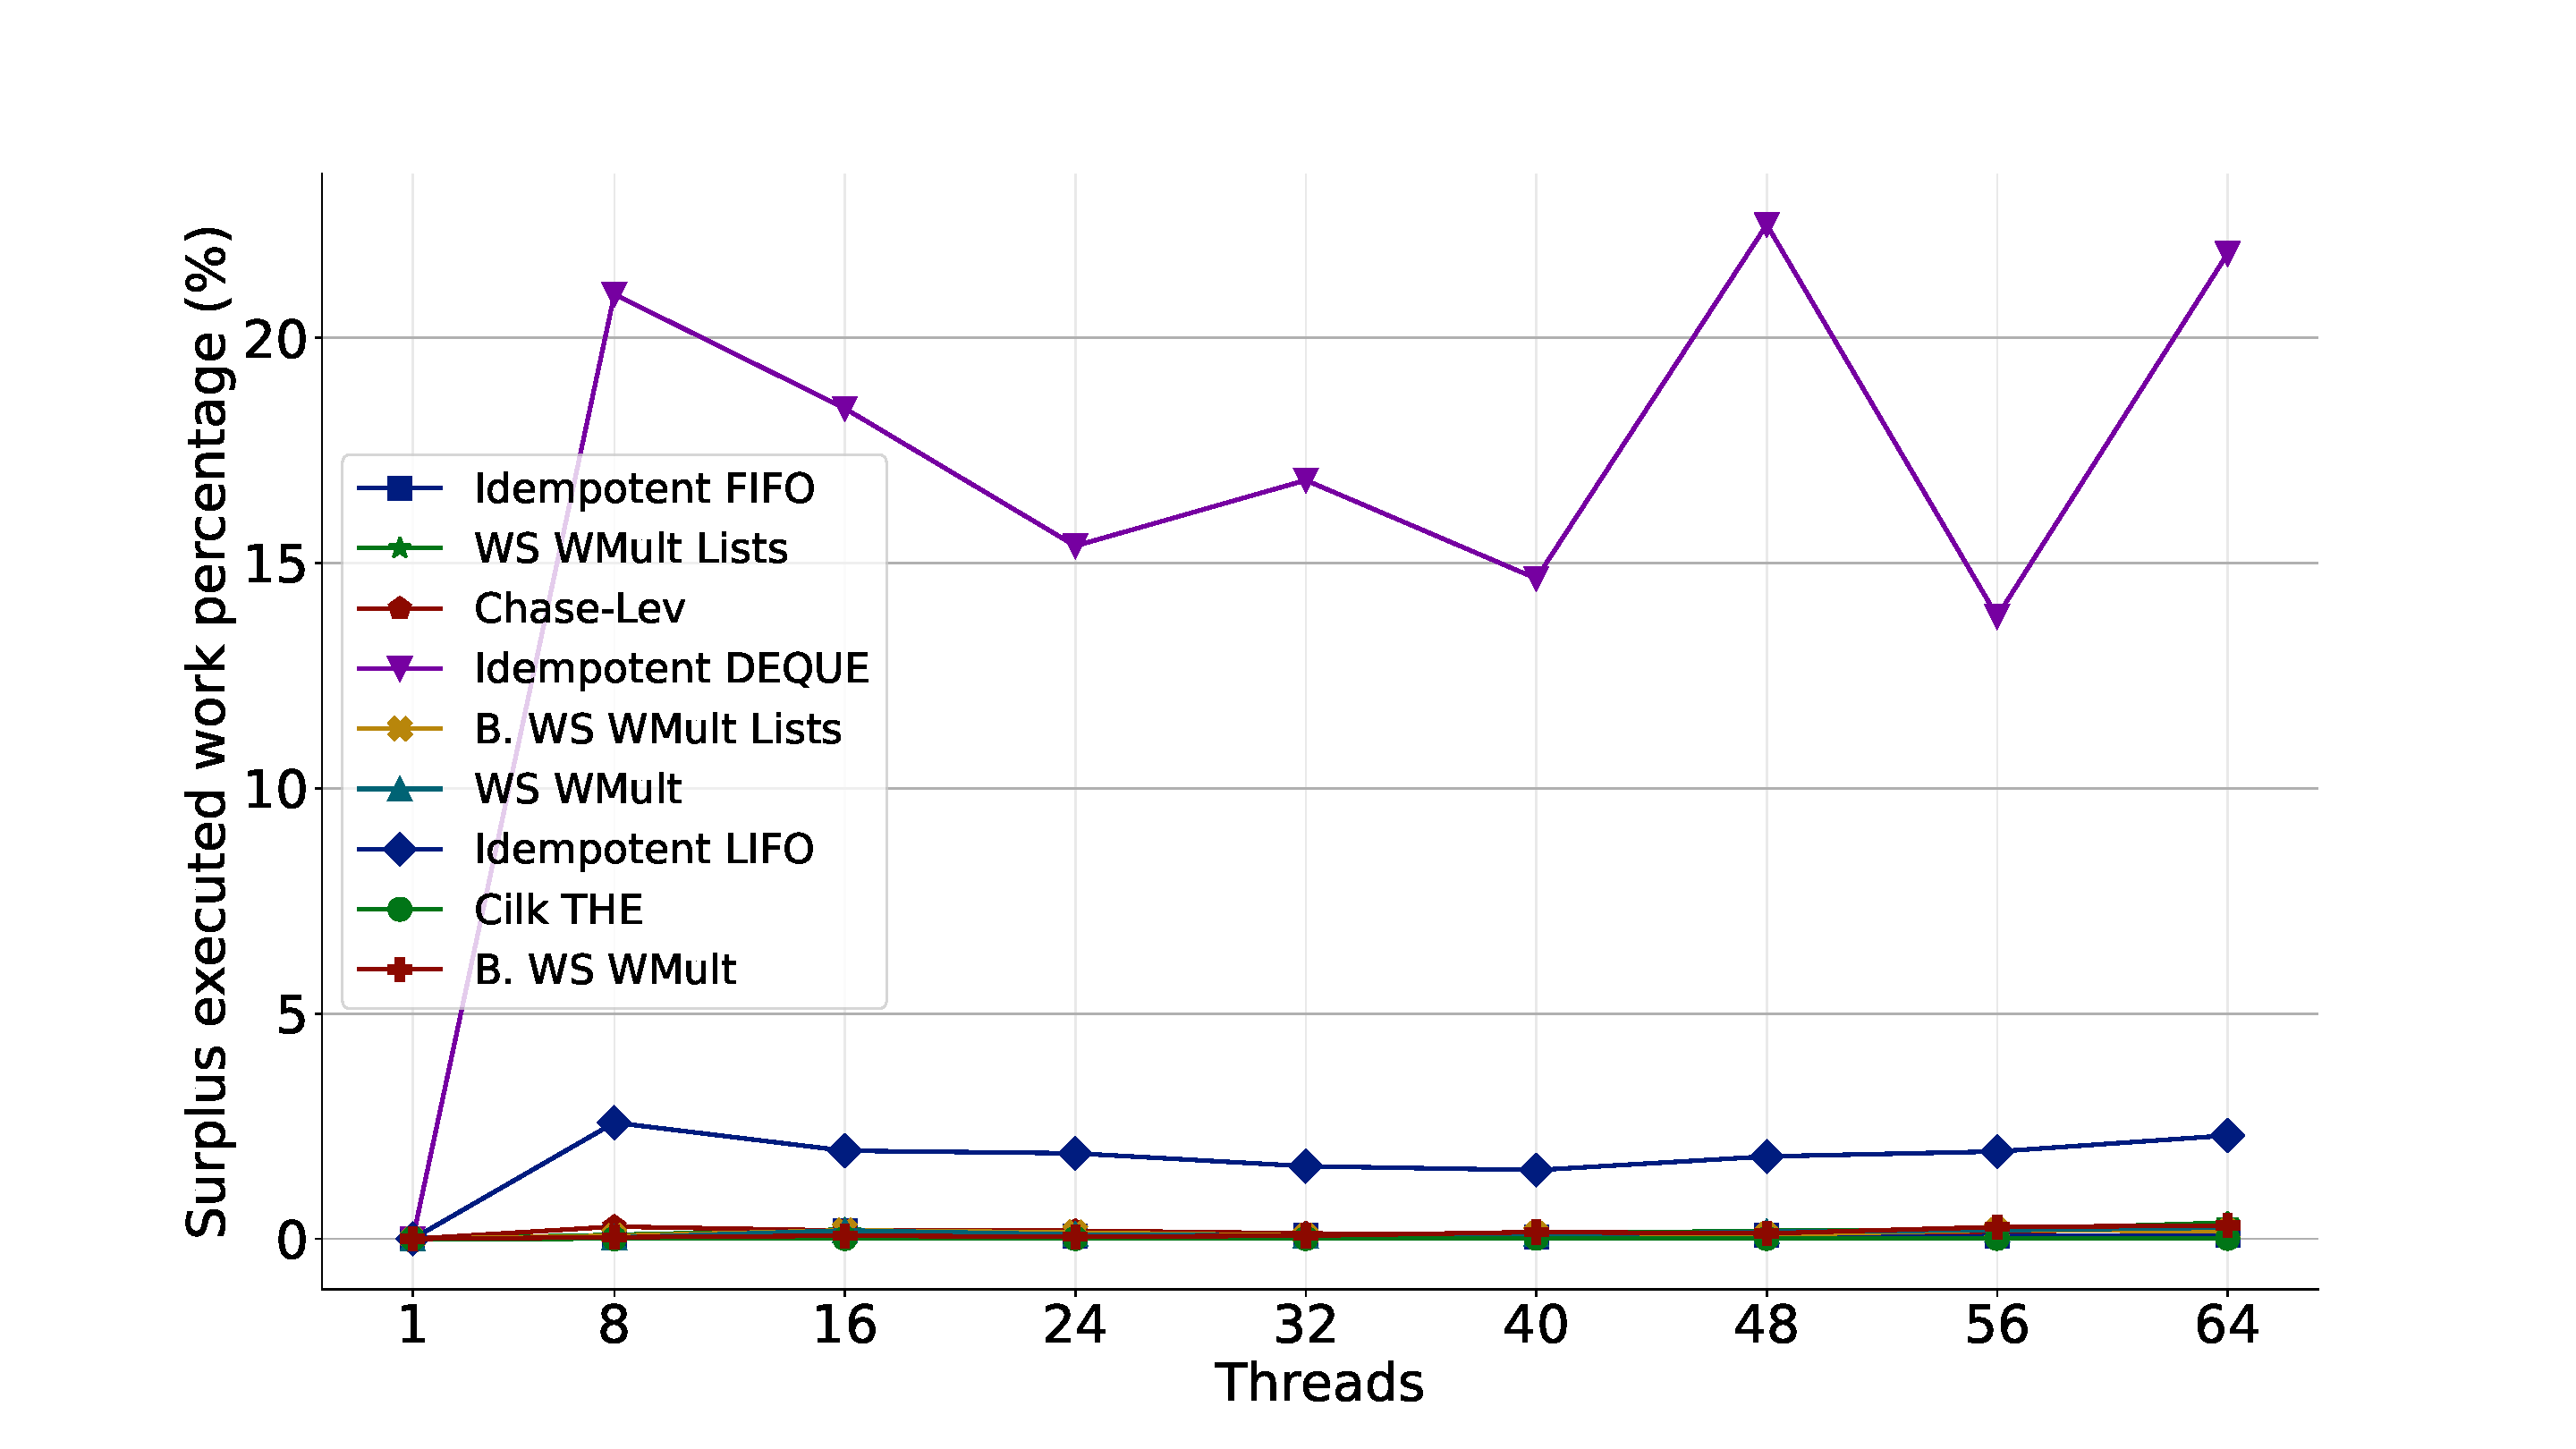
\includegraphics[width=0.48\textwidth]{contents/figures/IV_6_mult-exec-torus_3d_directed_256.pdf}
  }
  \subfloat[\label{fig:exec-surplustorus3ddirected:1000000}Executed surplus work: Directed Torus 3D. Initial size of 1,000,000 items.]{
    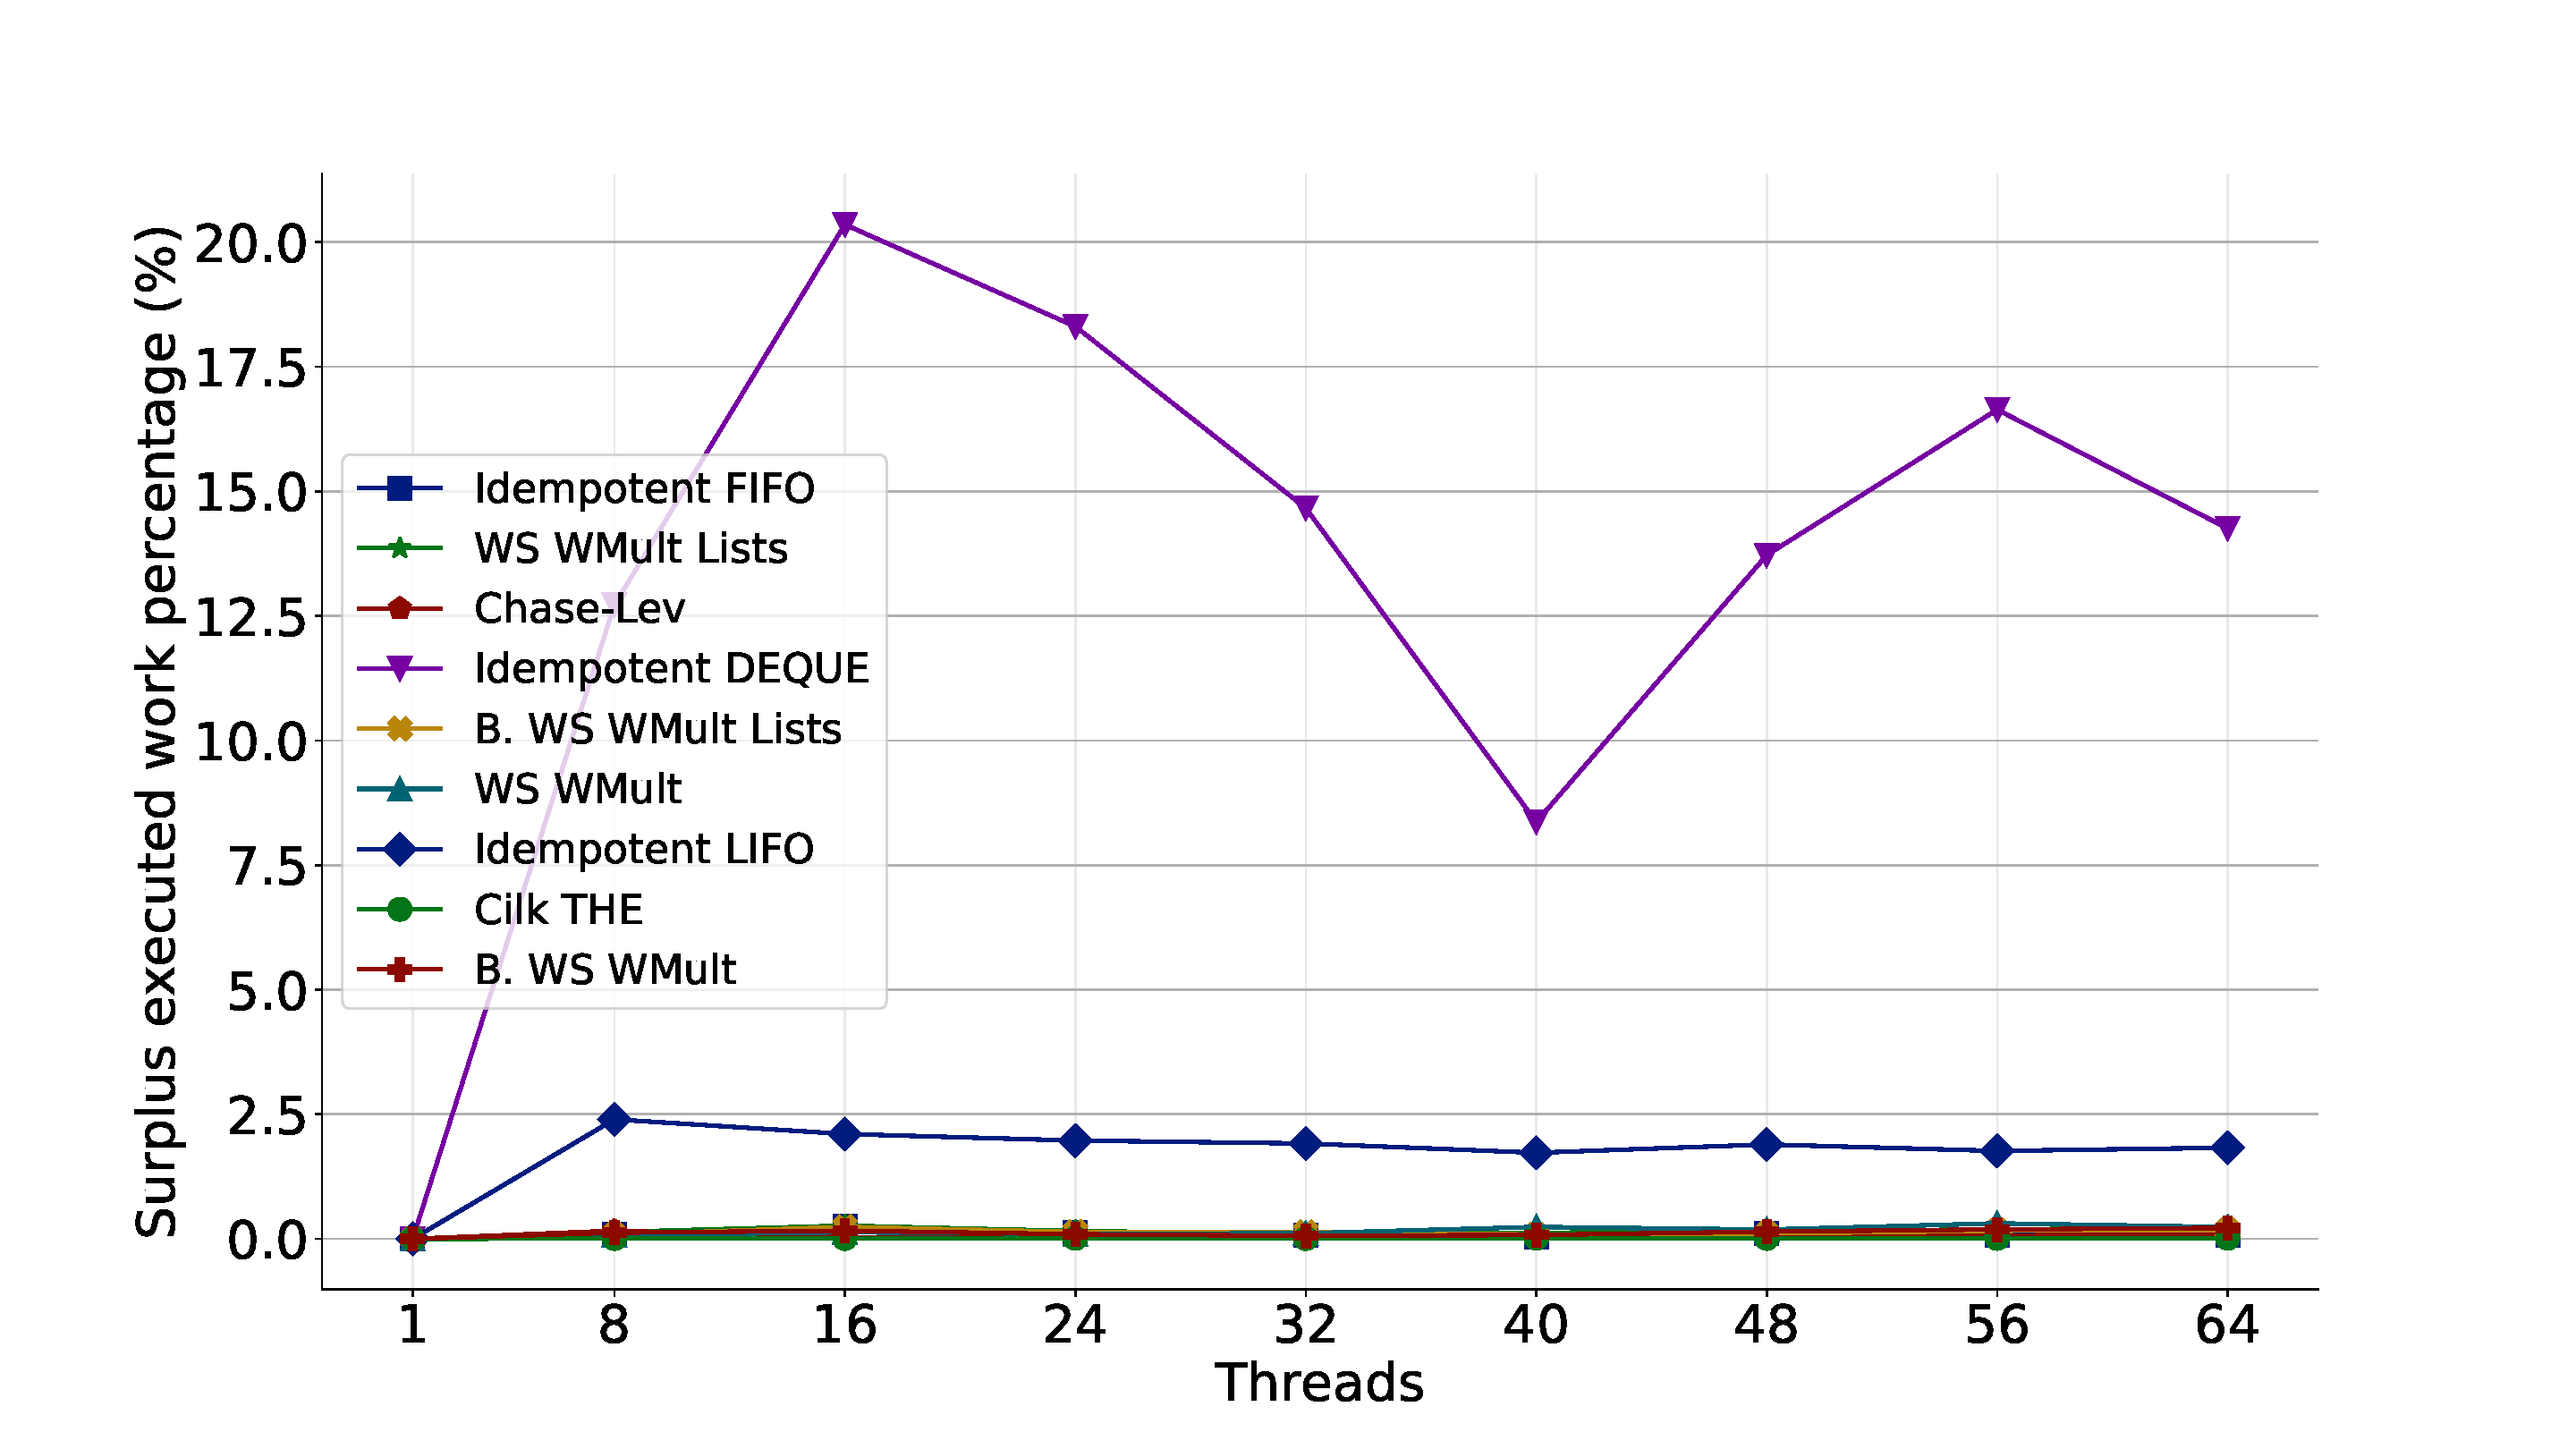
\includegraphics[width=0.48\textwidth]{contents/figures/IV_6_mult-exec-torus_3d_directed_1m.pdf}
  }

  \subfloat[\label{fig:exec-surplusrandom:256}Executed surplus work: Directed Random. Initial size of 256 items.]{
    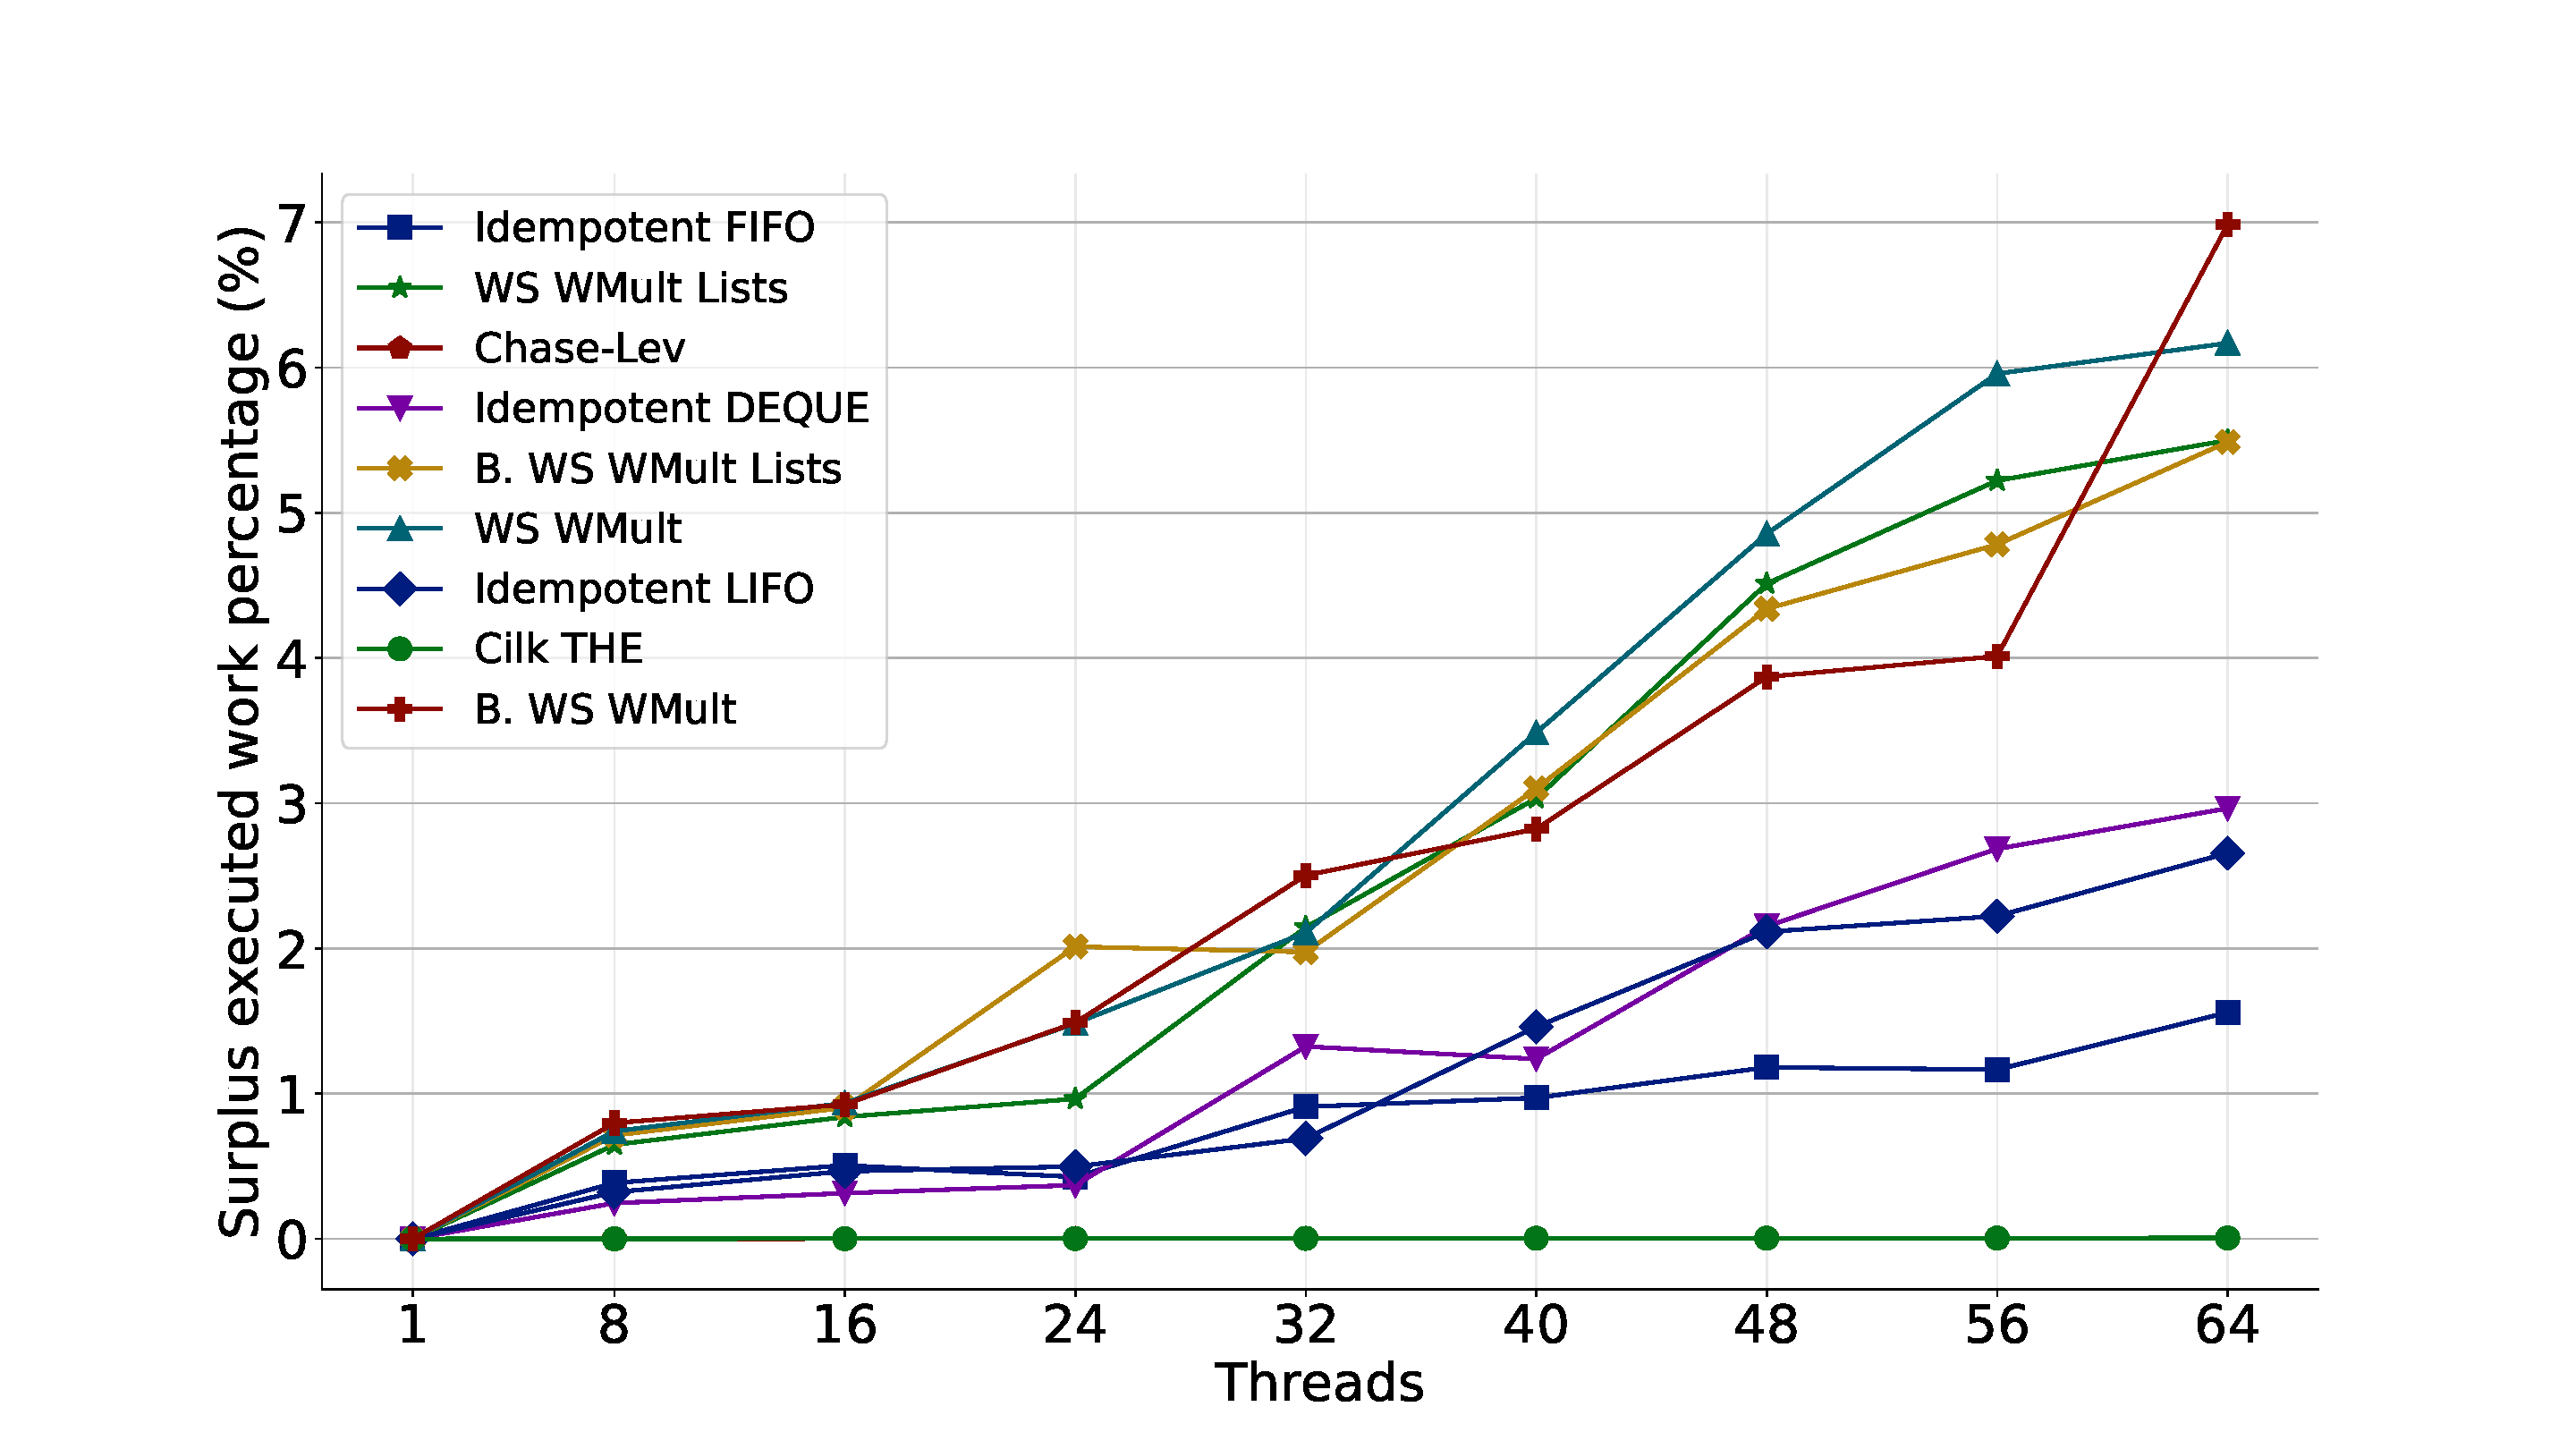
\includegraphics[width=0.48\textwidth]{contents/figures/IV_6_mult-exec-random_directed_256.pdf}
  }
  \subfloat[\label{fig:exec-surplusrandom:1000000}Executed surplus work: Directed Random: Initial size of 1,000,000 items.]{
    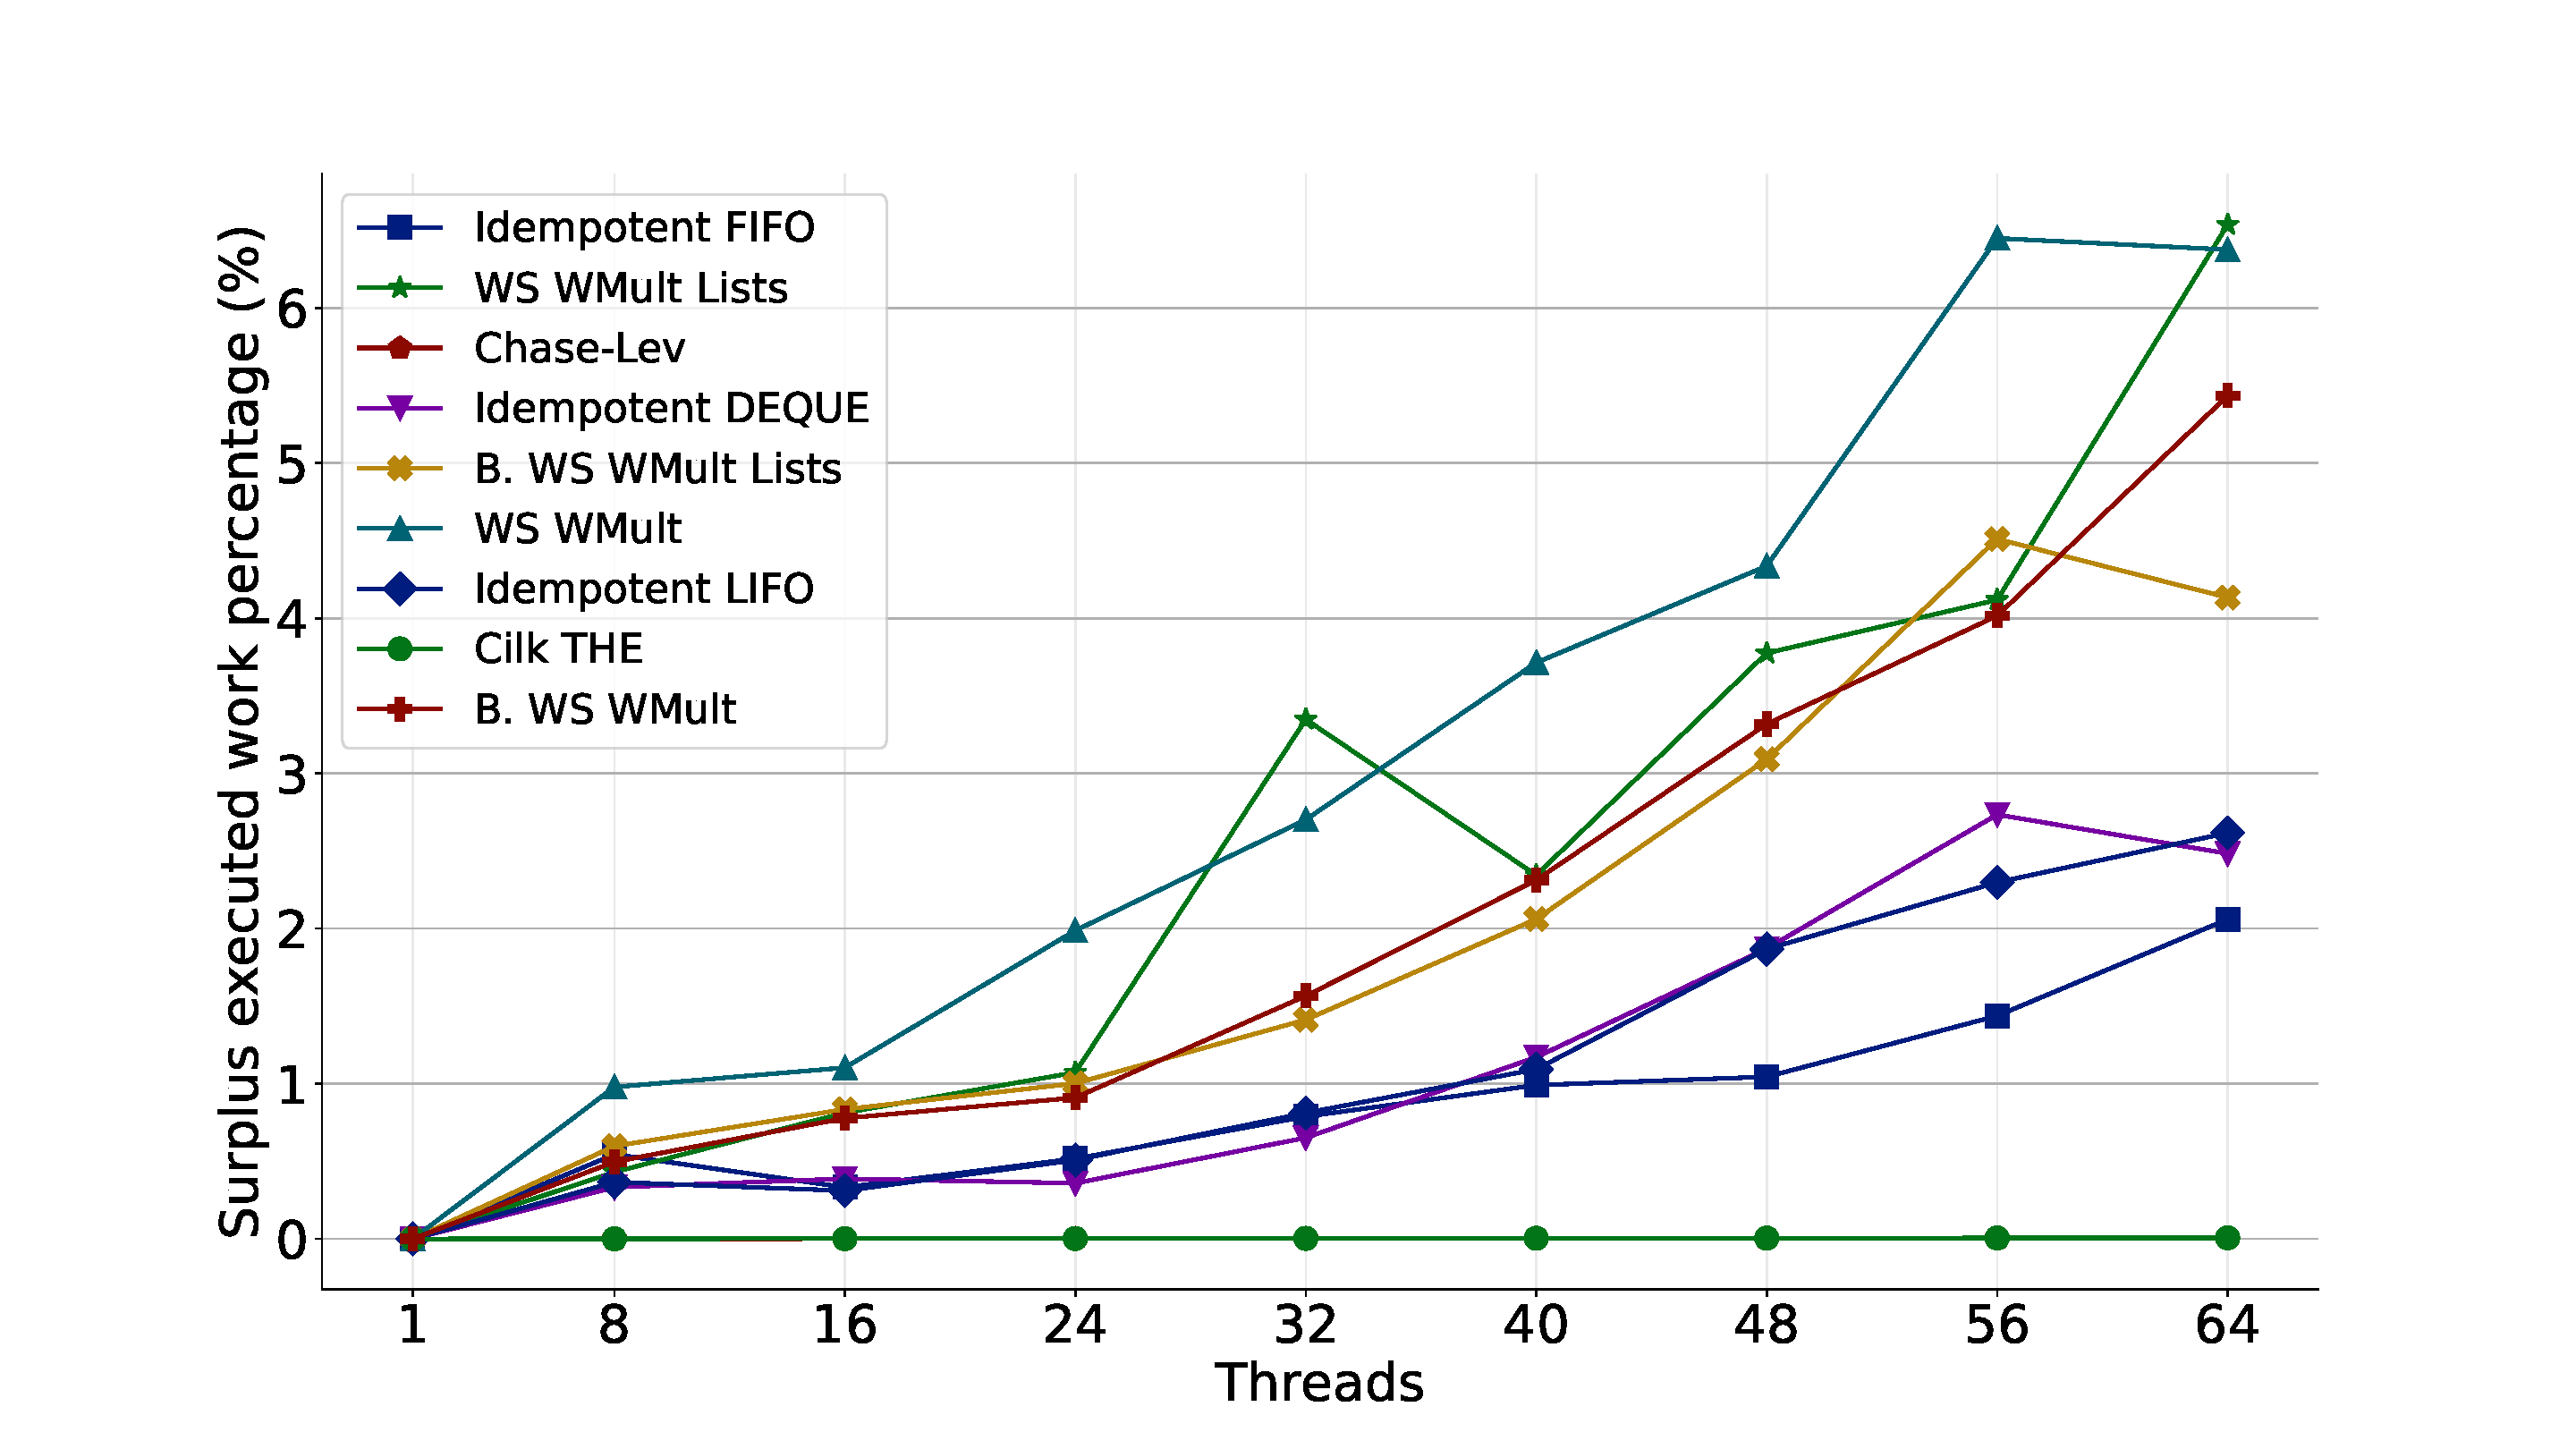
\includegraphics[width=0.48\textwidth]{contents/figures/IV_6_mult-exec-random_directed_1m.pdf}
  }

  \caption{\label{fig:exec-surplusgraphapplication} Executed surplus work (percentage) of the experiments. Surplus work: the difference between the total number of \Takes and the number of takes in sequential executions (i.e., $1,000,000$).}

\end{figure}

\begin{figure}[!ht]
  \subfloat[\label{fig:sat:50:1}Range assignment size 50.]{
    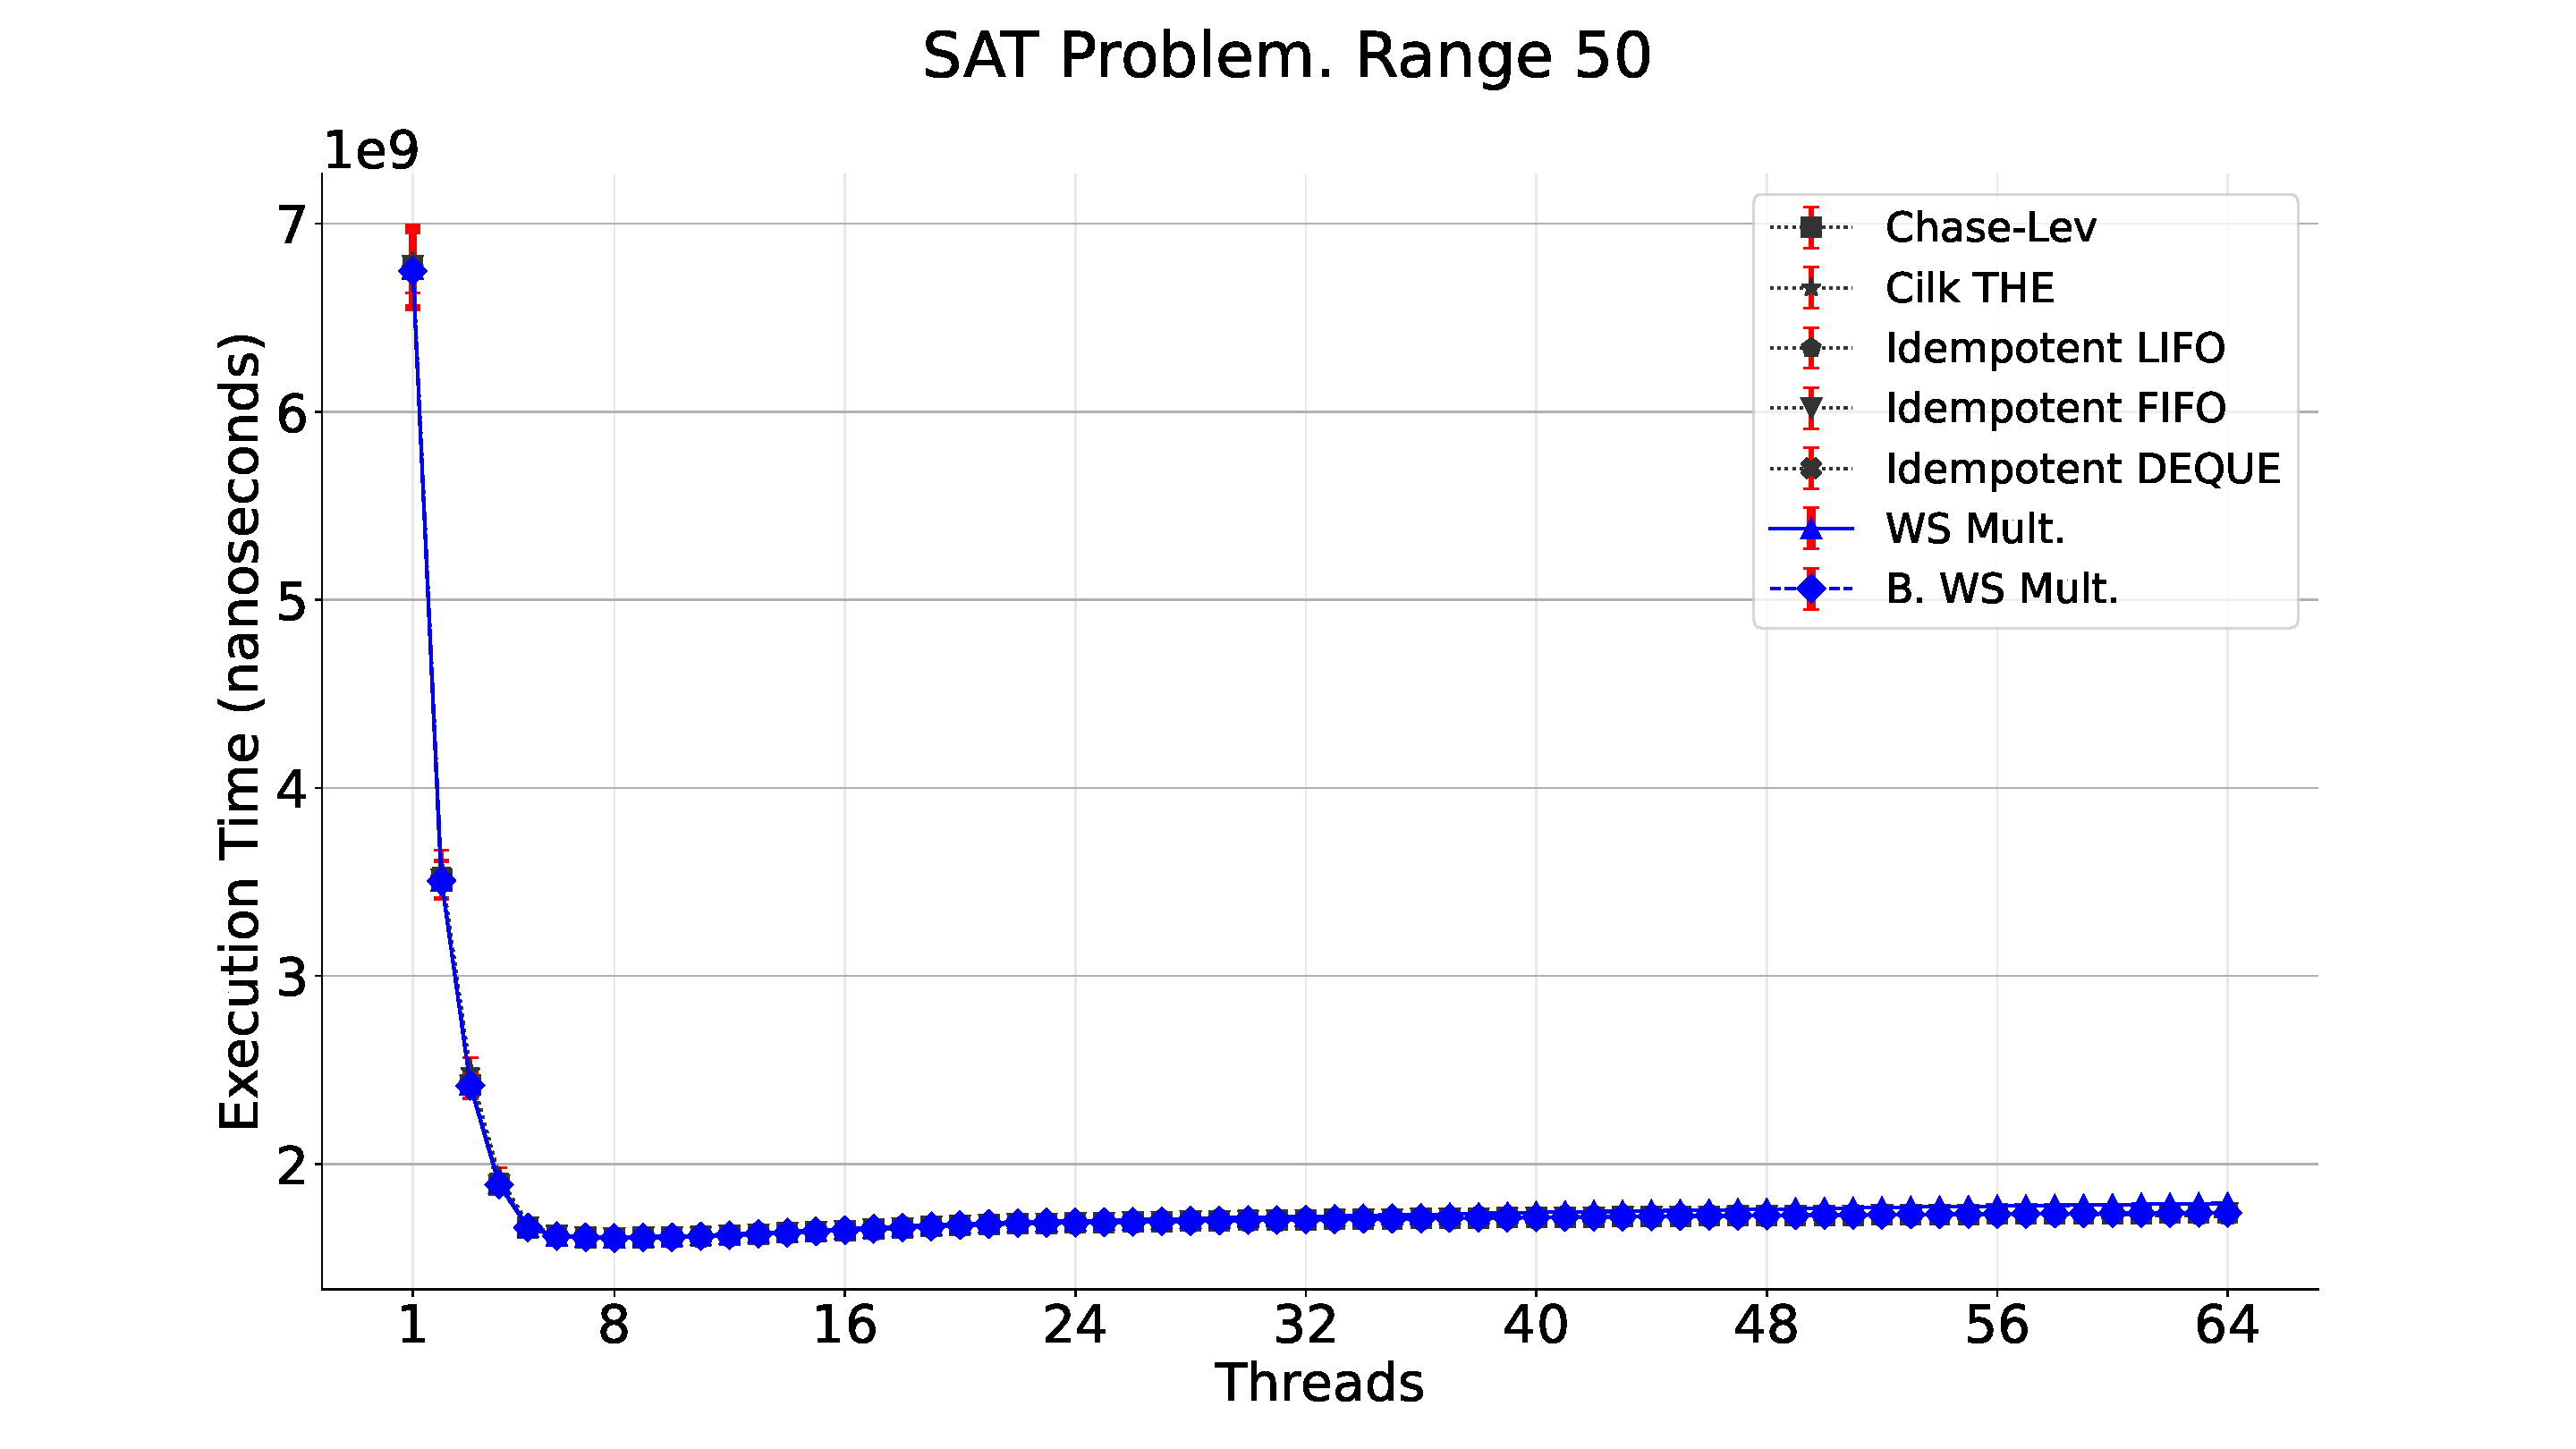
\includegraphics[width=0.48\textwidth]{contents/figures/IV_6_sat-50-1.pdf}
  }
  \subfloat[\label{fig:sat:50:2}Range assignment size 50. Zoom in to the number of processes 32 to 64.]{
    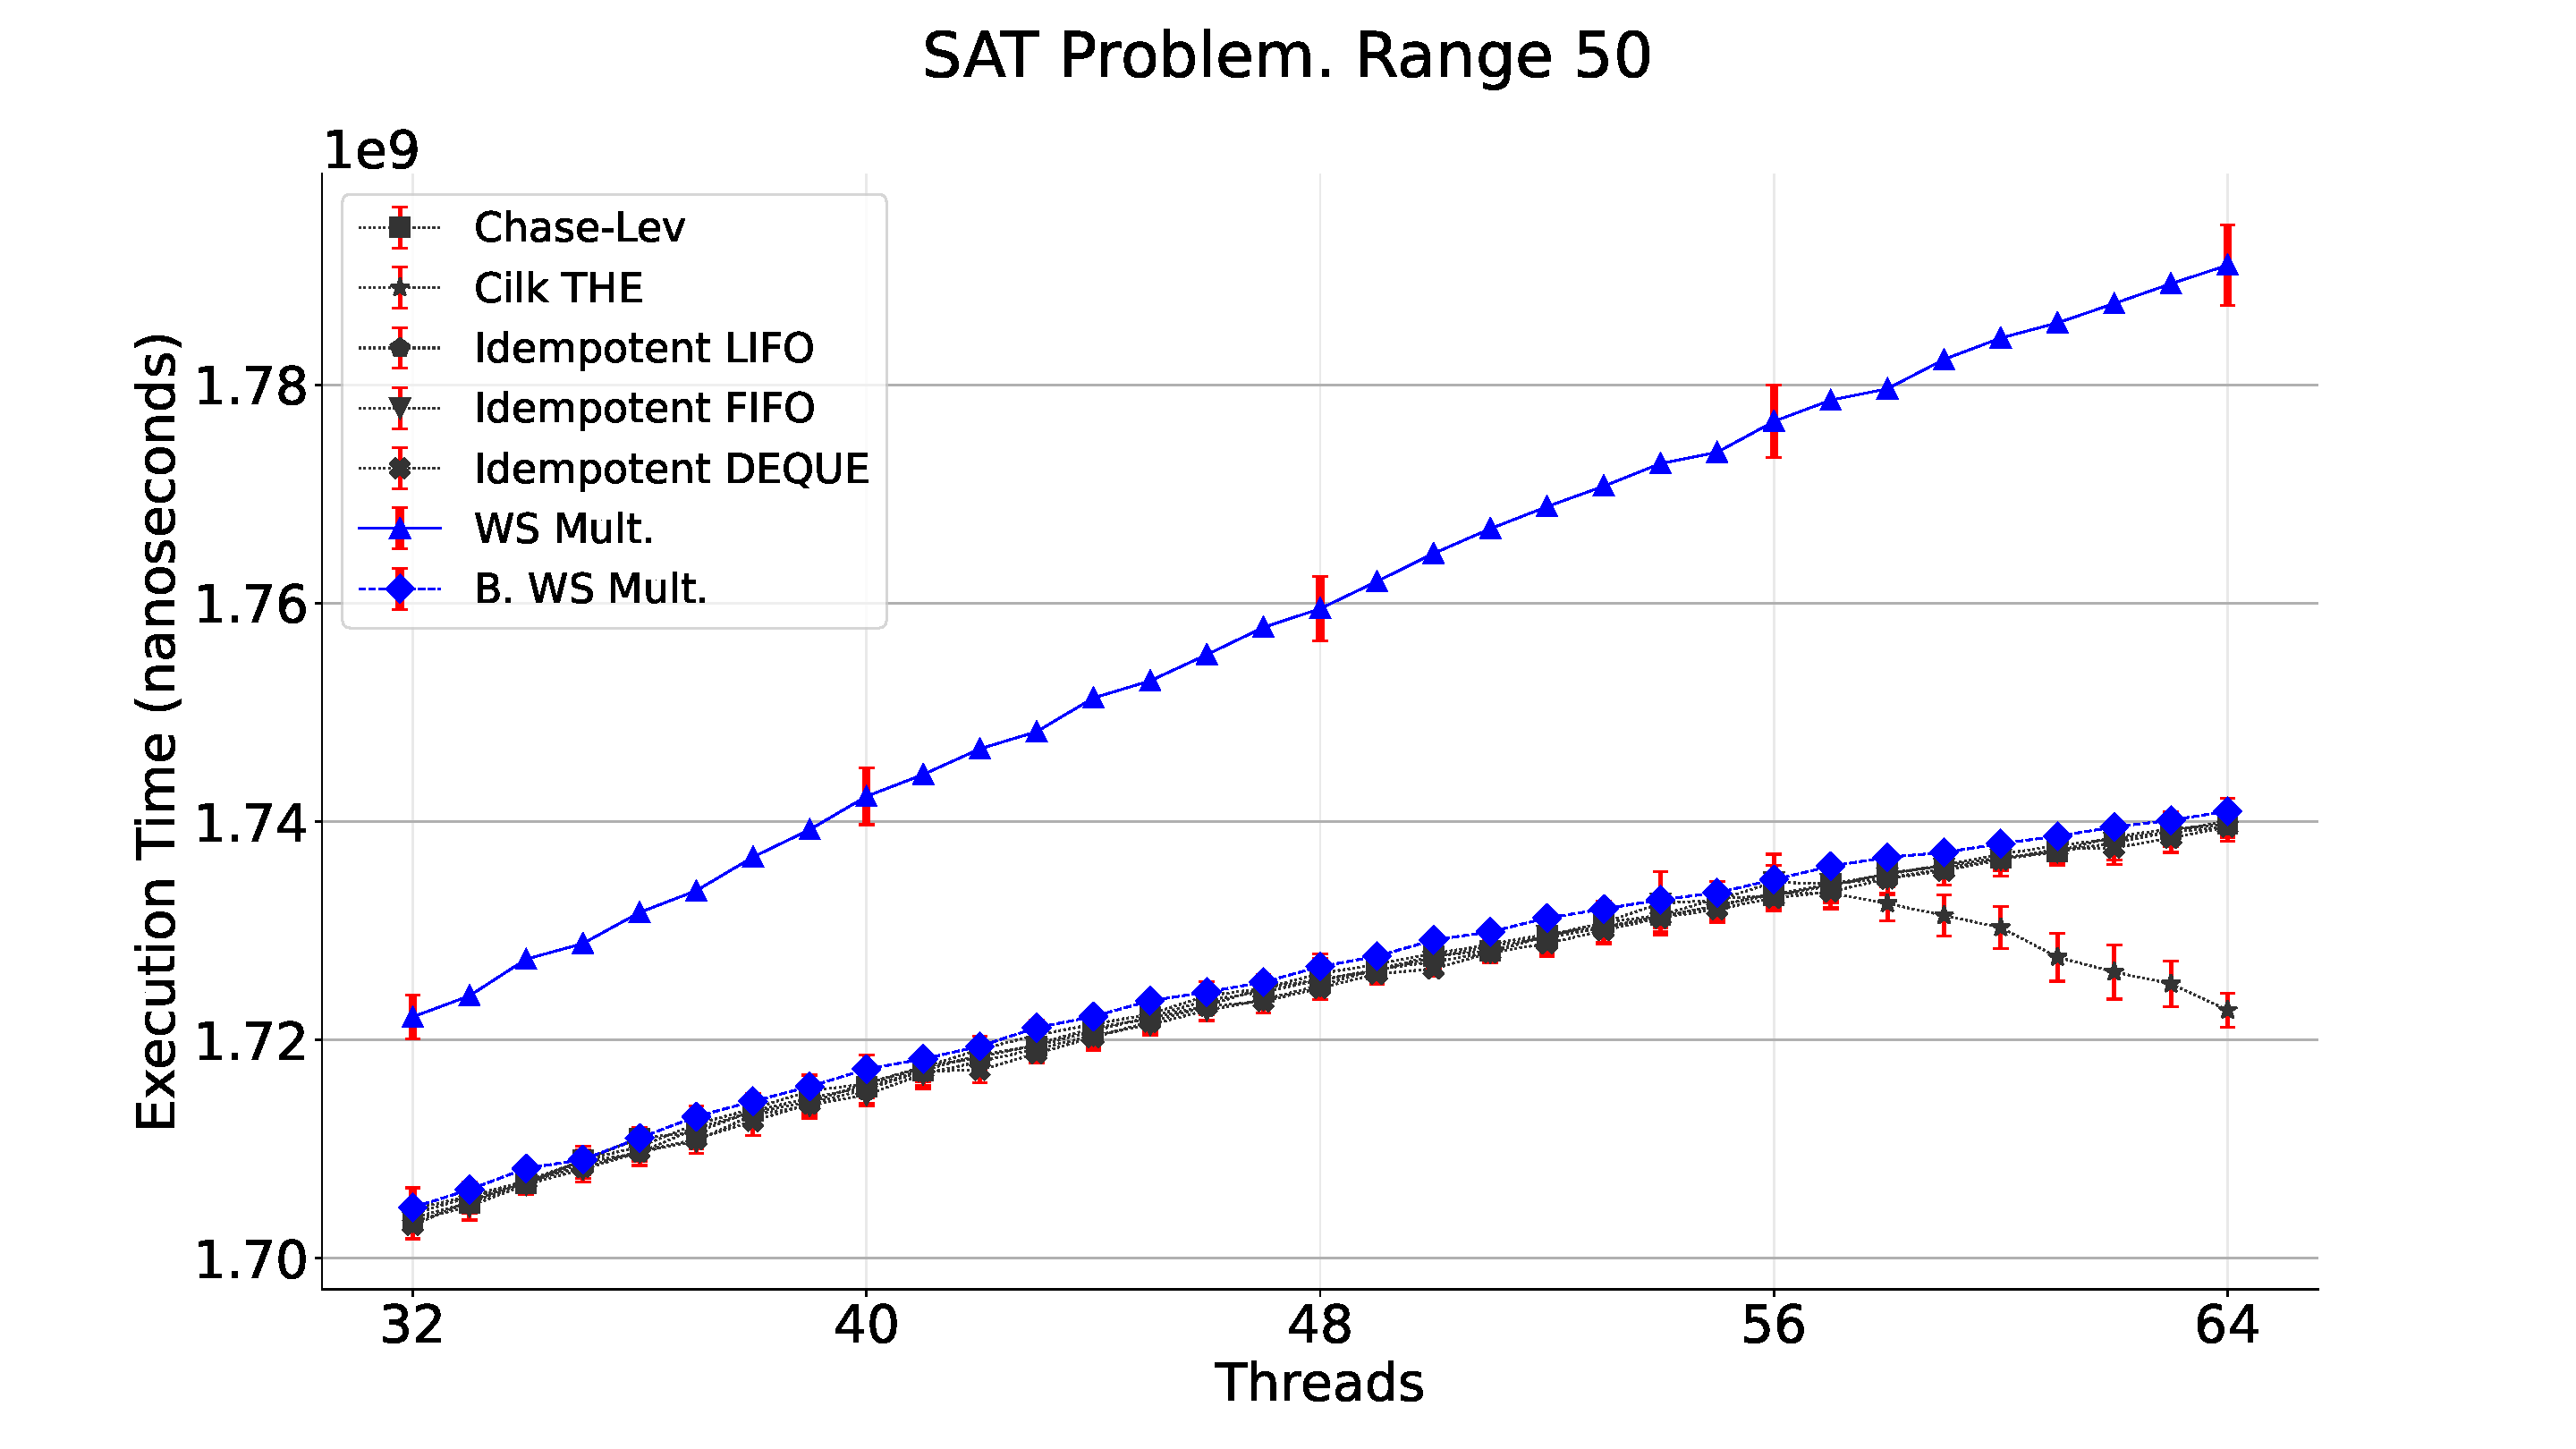
\includegraphics[width=0.48\textwidth]{contents/figures/IV_6_sat-50-2.pdf}
  }

  \subfloat[\label{fig:sat:250:1}Range assignment size 250.]{
    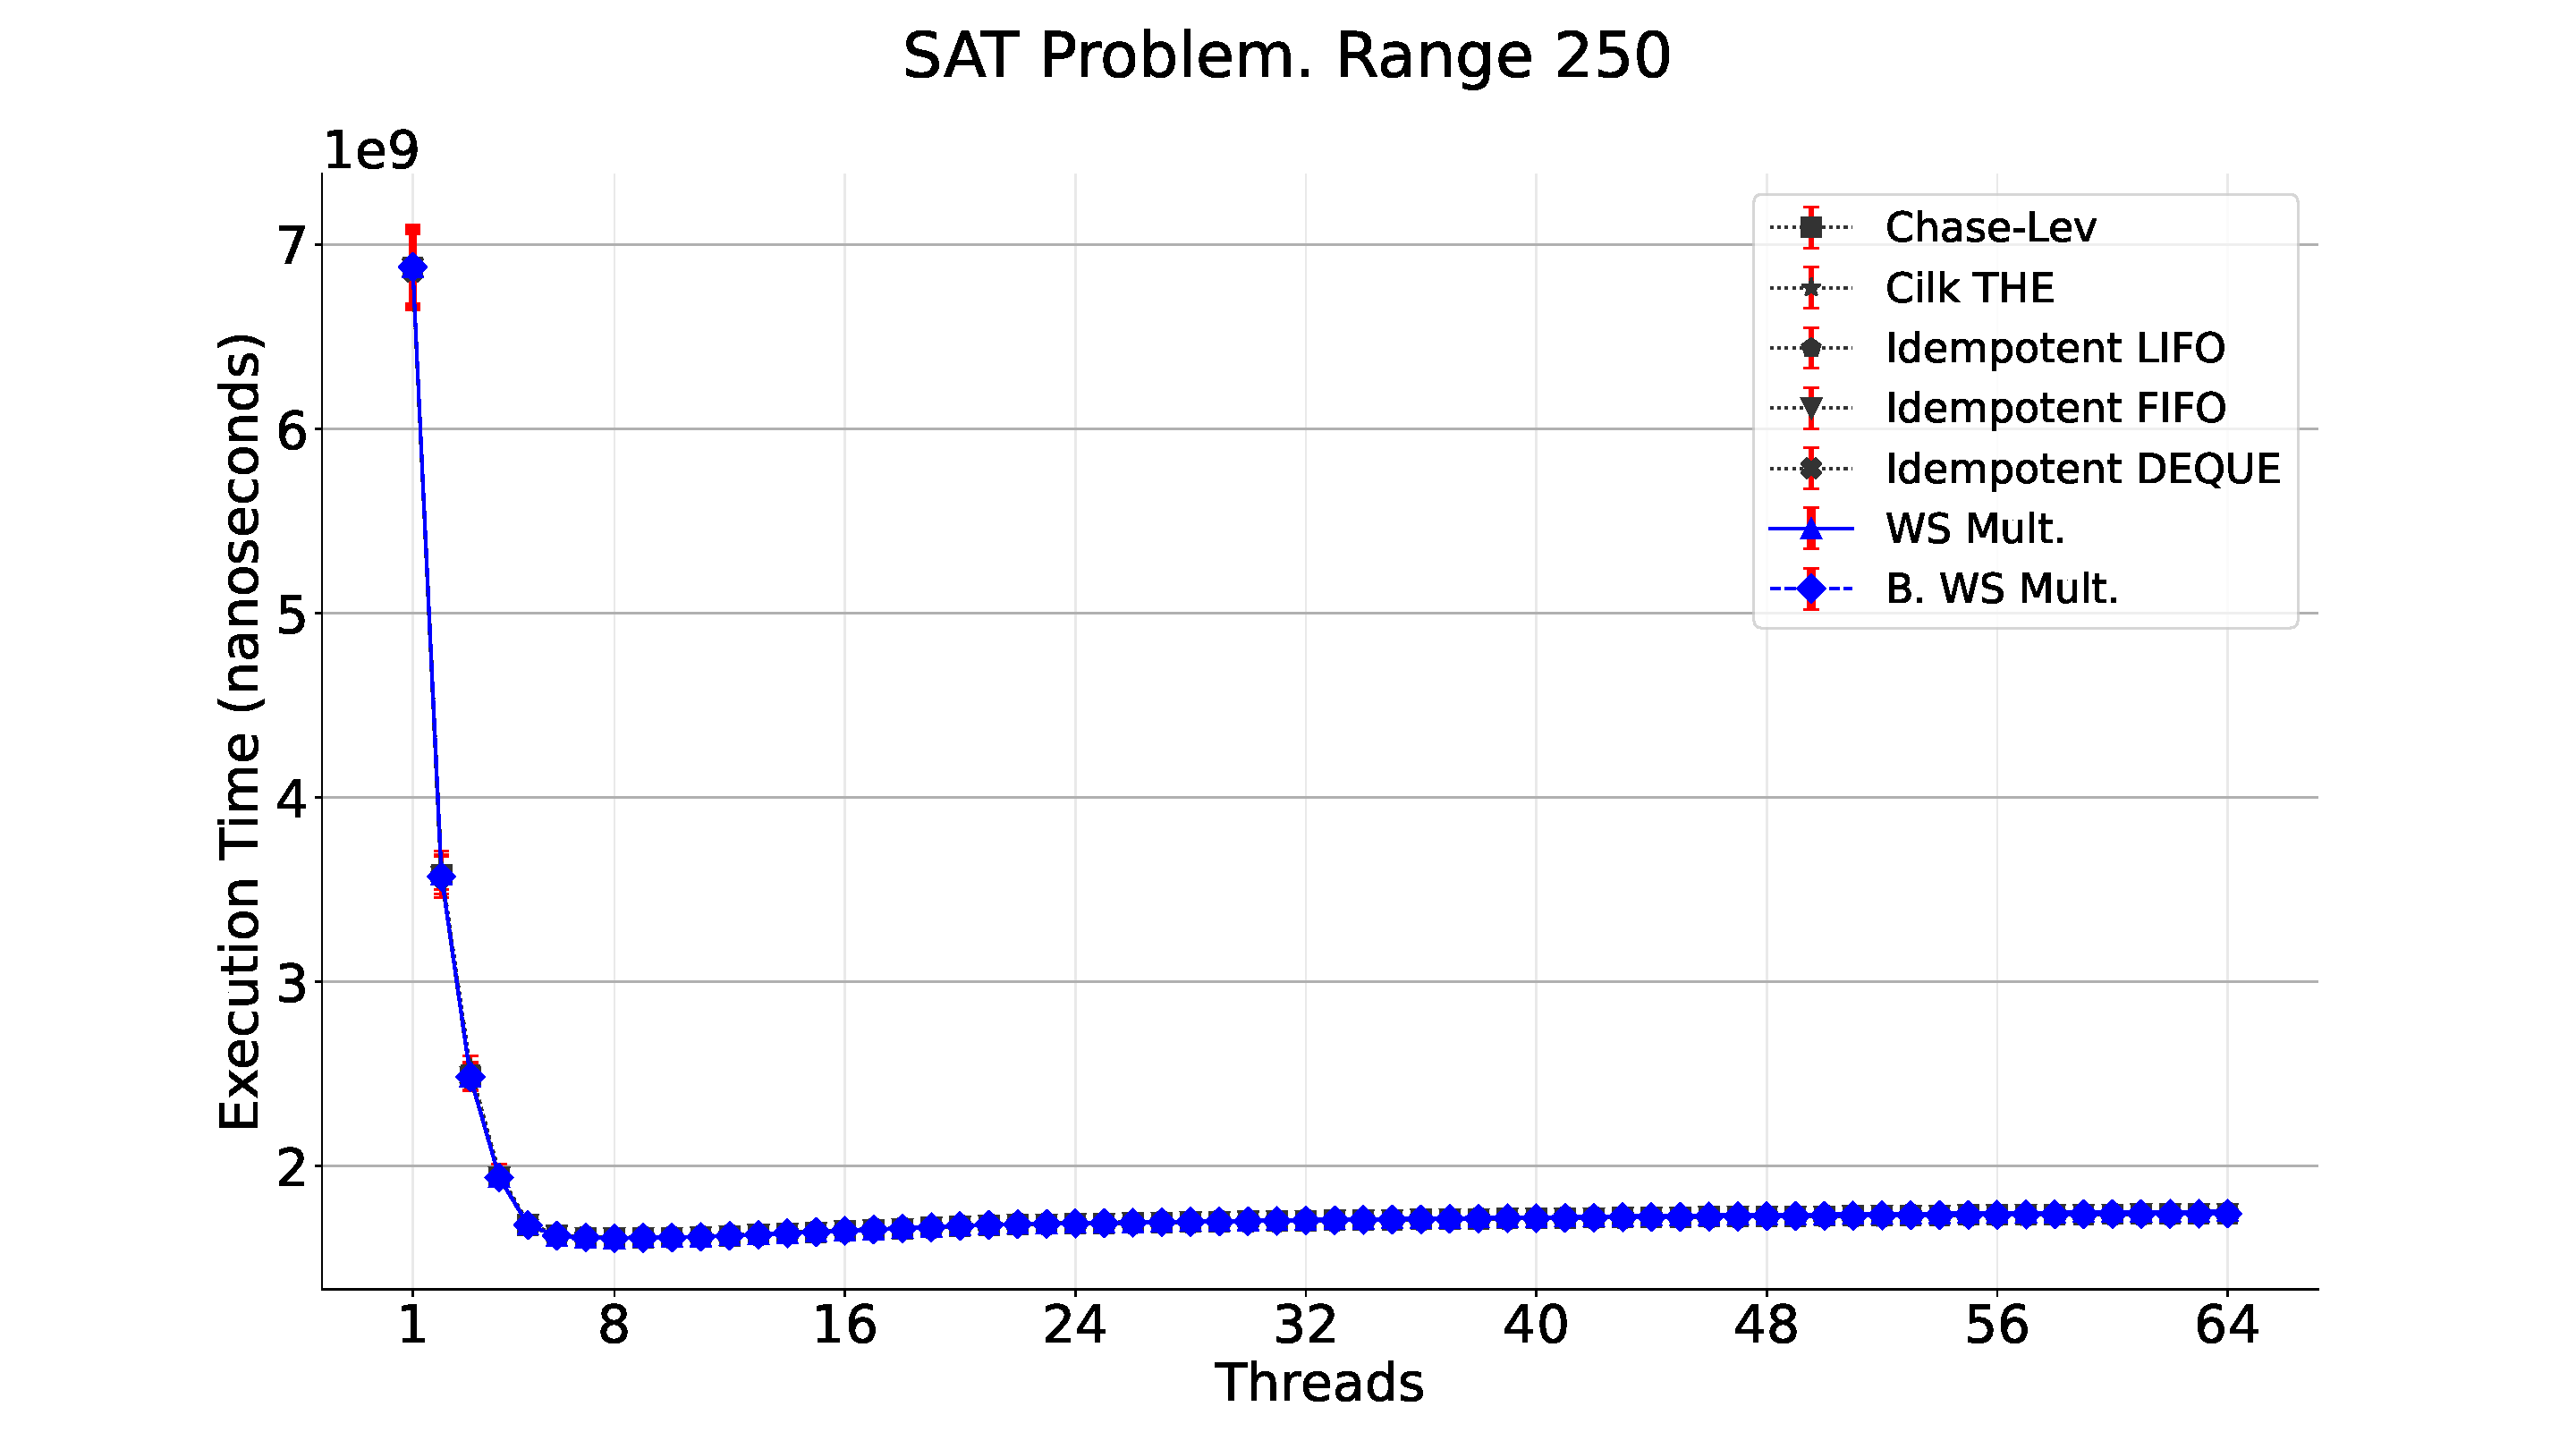
\includegraphics[width=0.48\textwidth]{contents/figures/IV_6_sat-250-1.pdf}
  }
  \subfloat[\label{fig:sat:250:2}Range assignment size 250. Zoom in to the number of processes 32 to 64.]{
    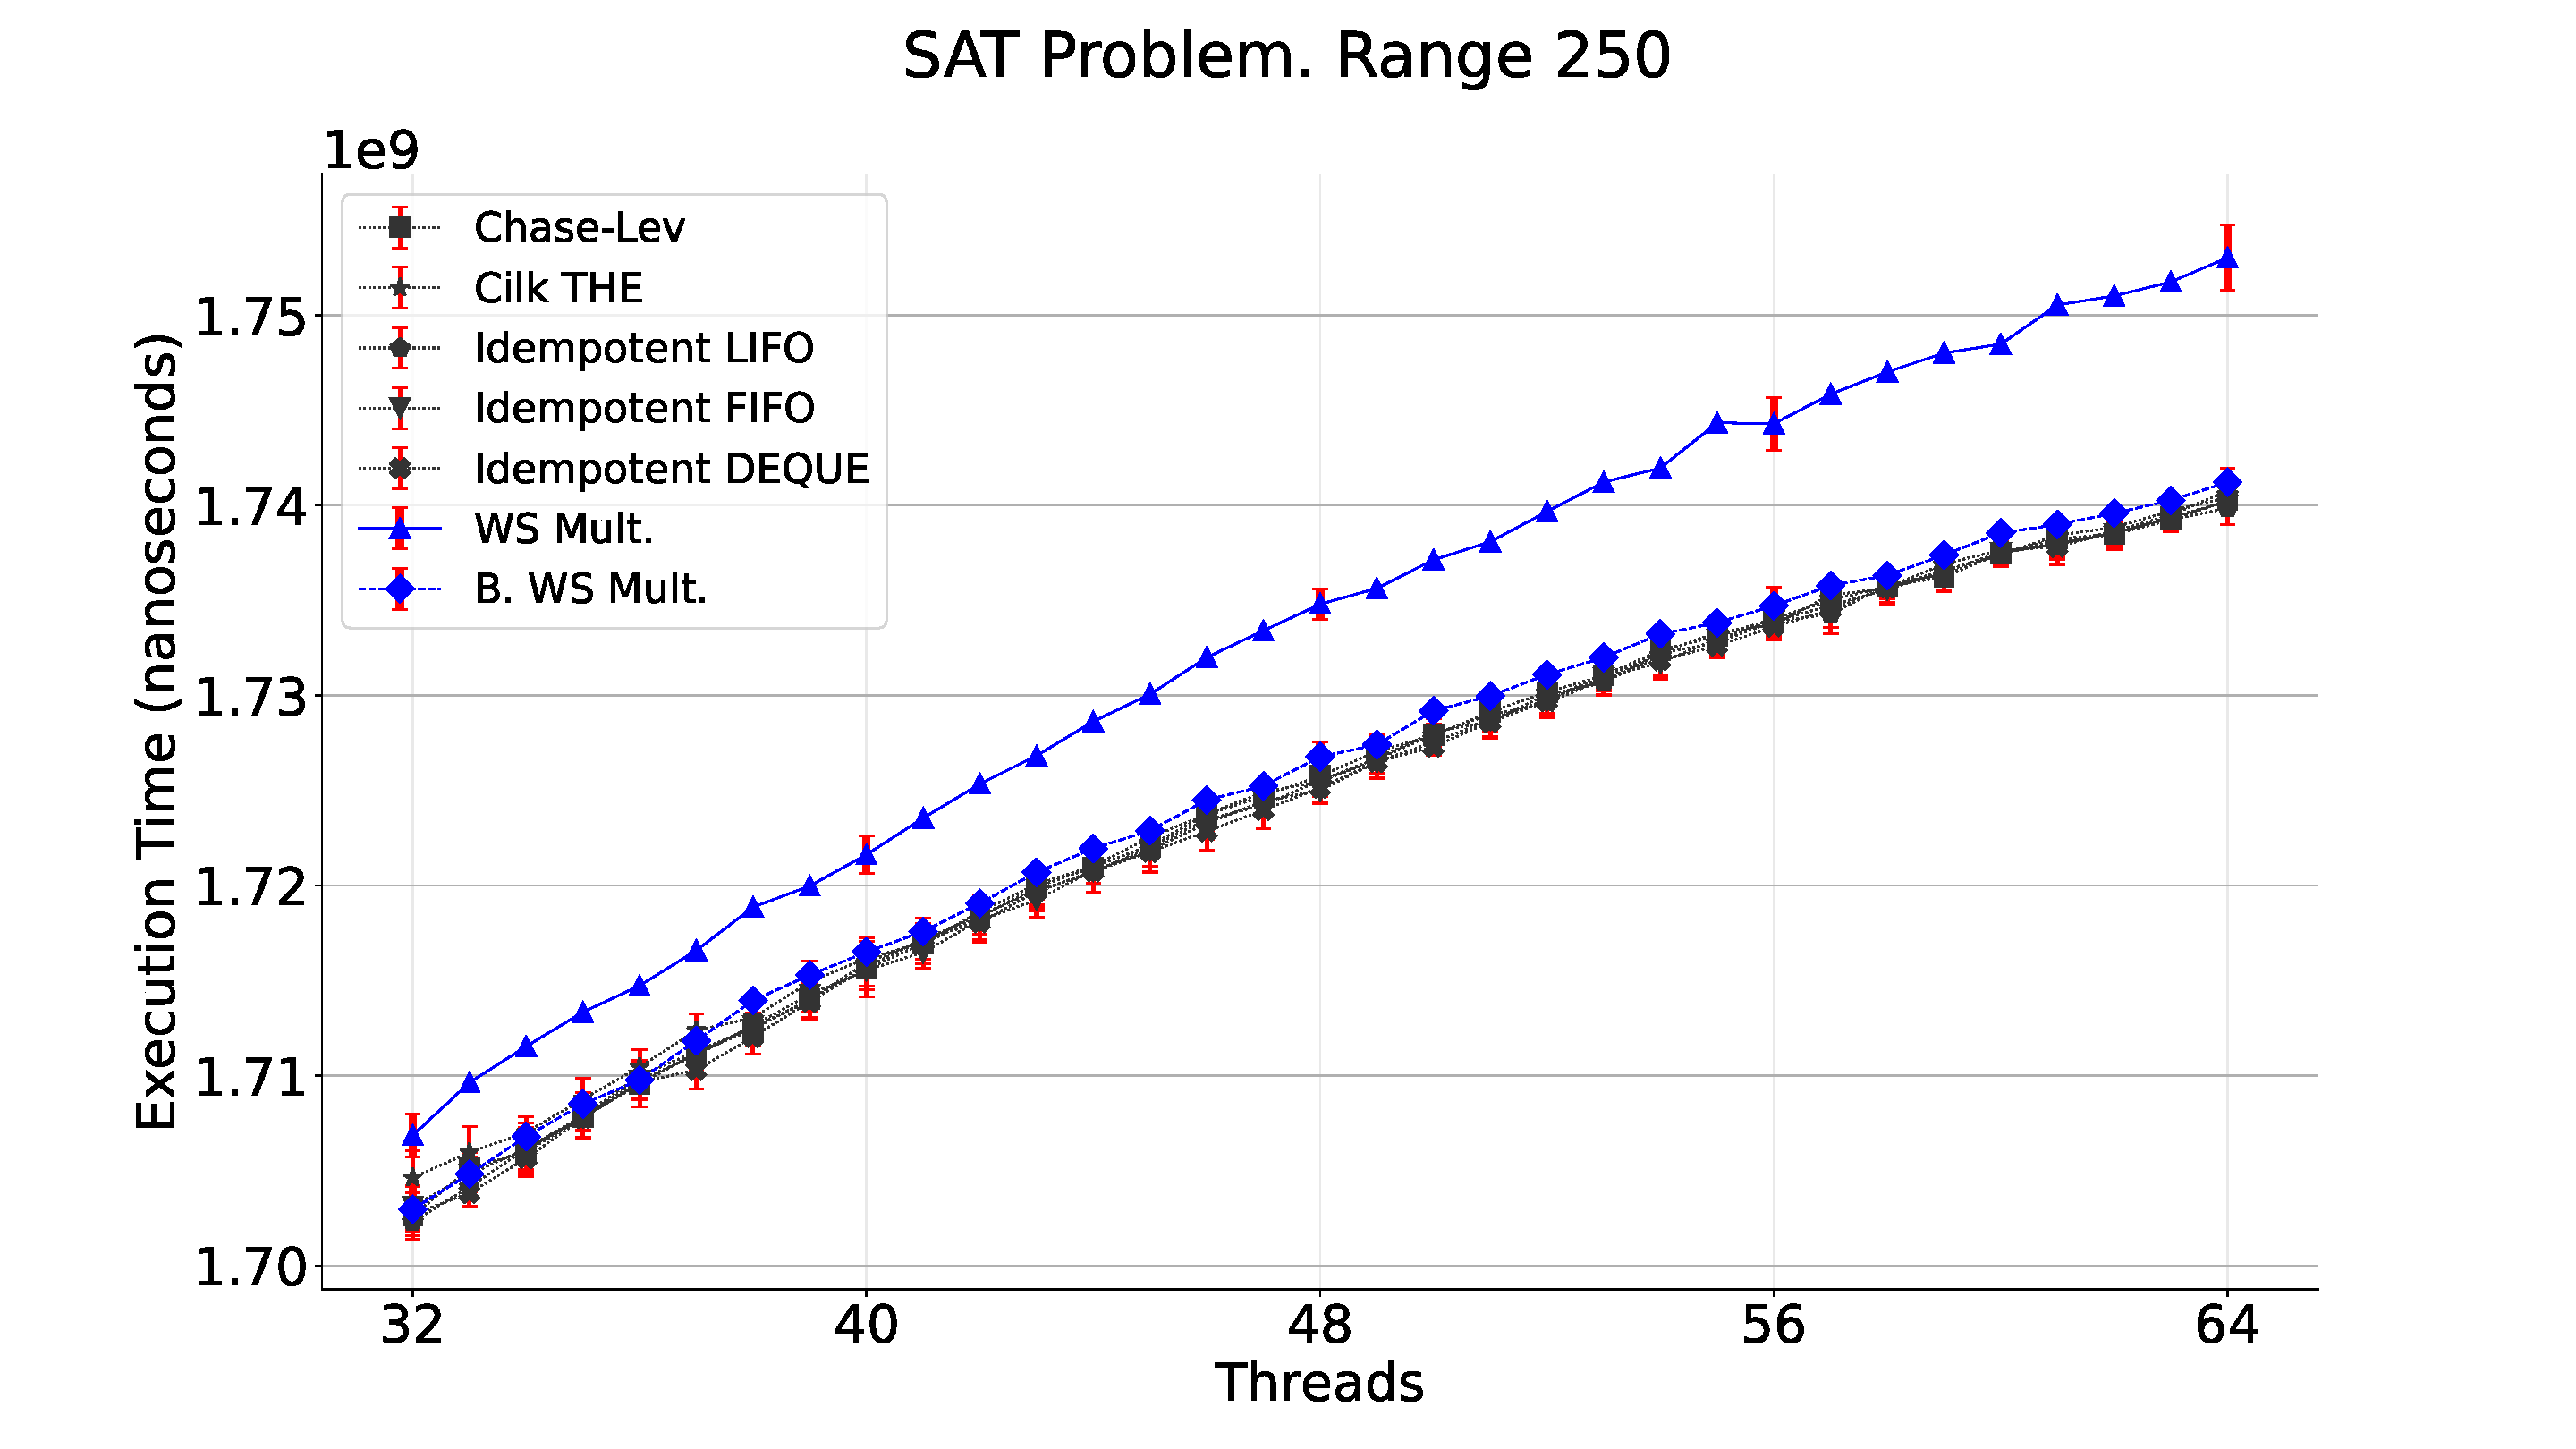
\includegraphics[width=0.48\textwidth]{contents/figures/IV_6_sat-250-2.pdf}
  }

  \subfloat[\label{fig:sat:1000:1}Range assignment size 1,000.]{
    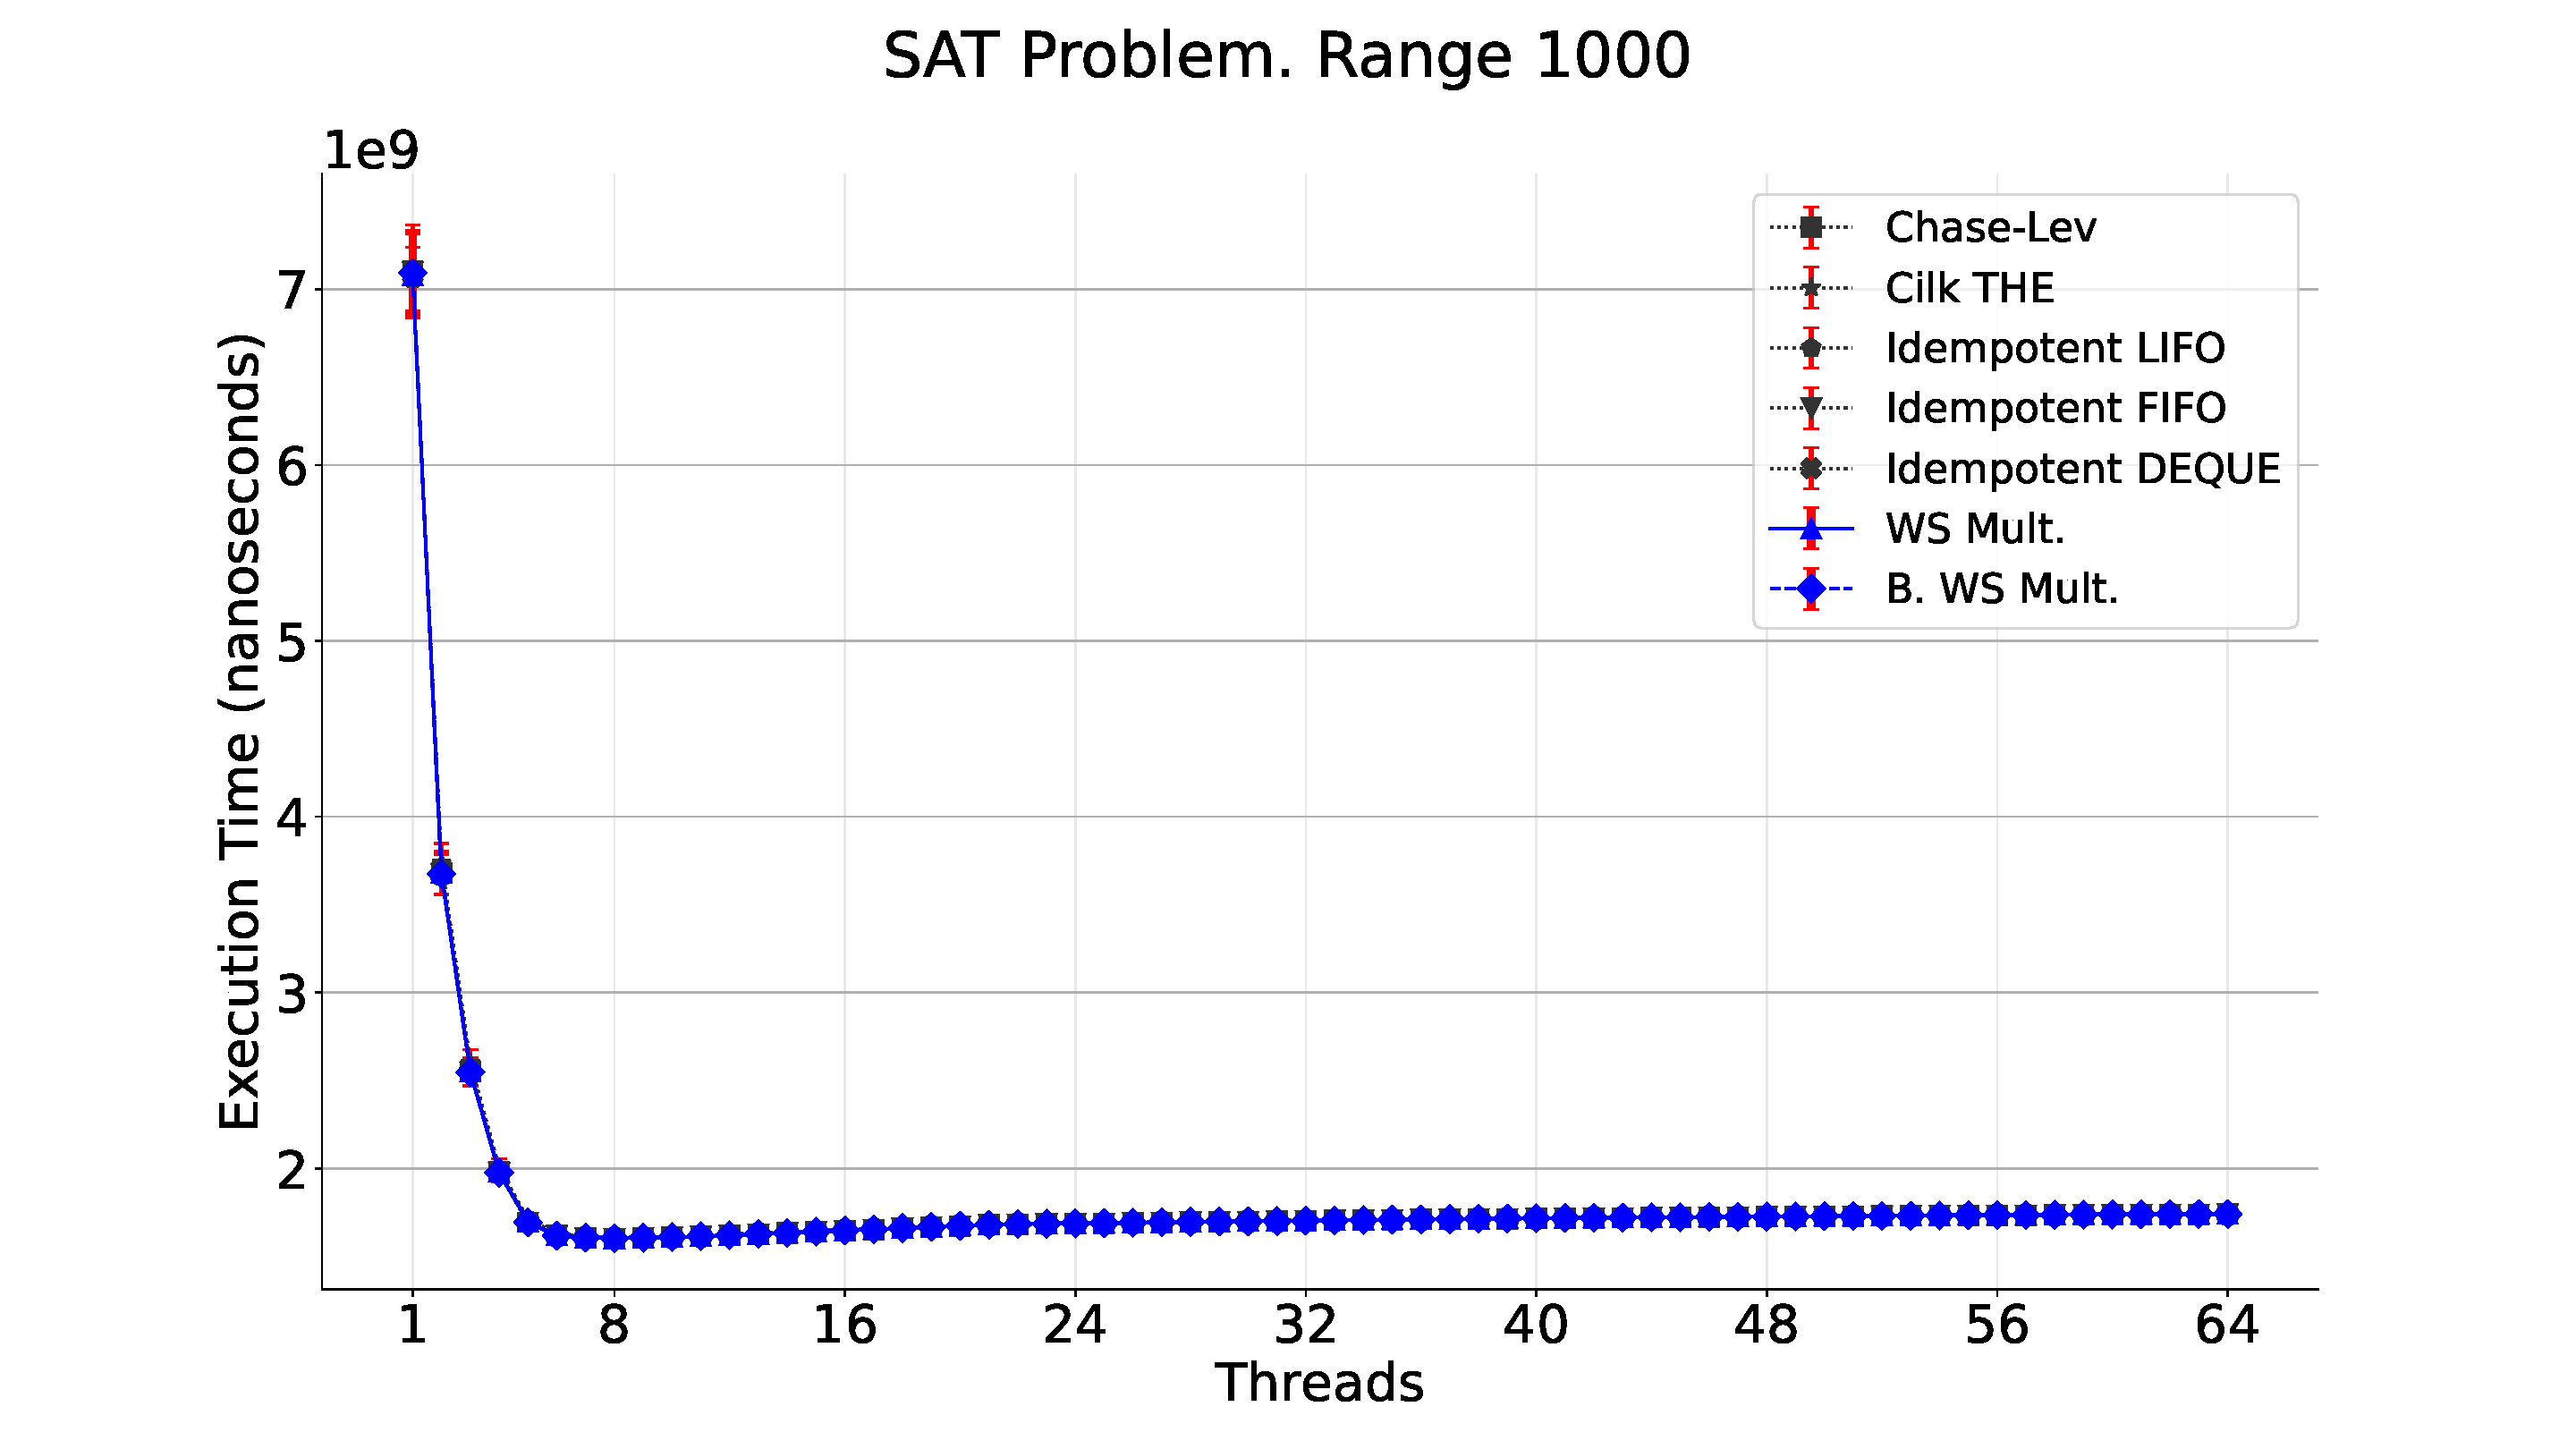
\includegraphics[width=0.48\textwidth]{contents/figures/IV_6_sat-1000-1.pdf}
  }
  \subfloat[\label{fig:sat:1000:2}Range assignment size 1,000. Zoom in to several processes 32 to 64.]{
    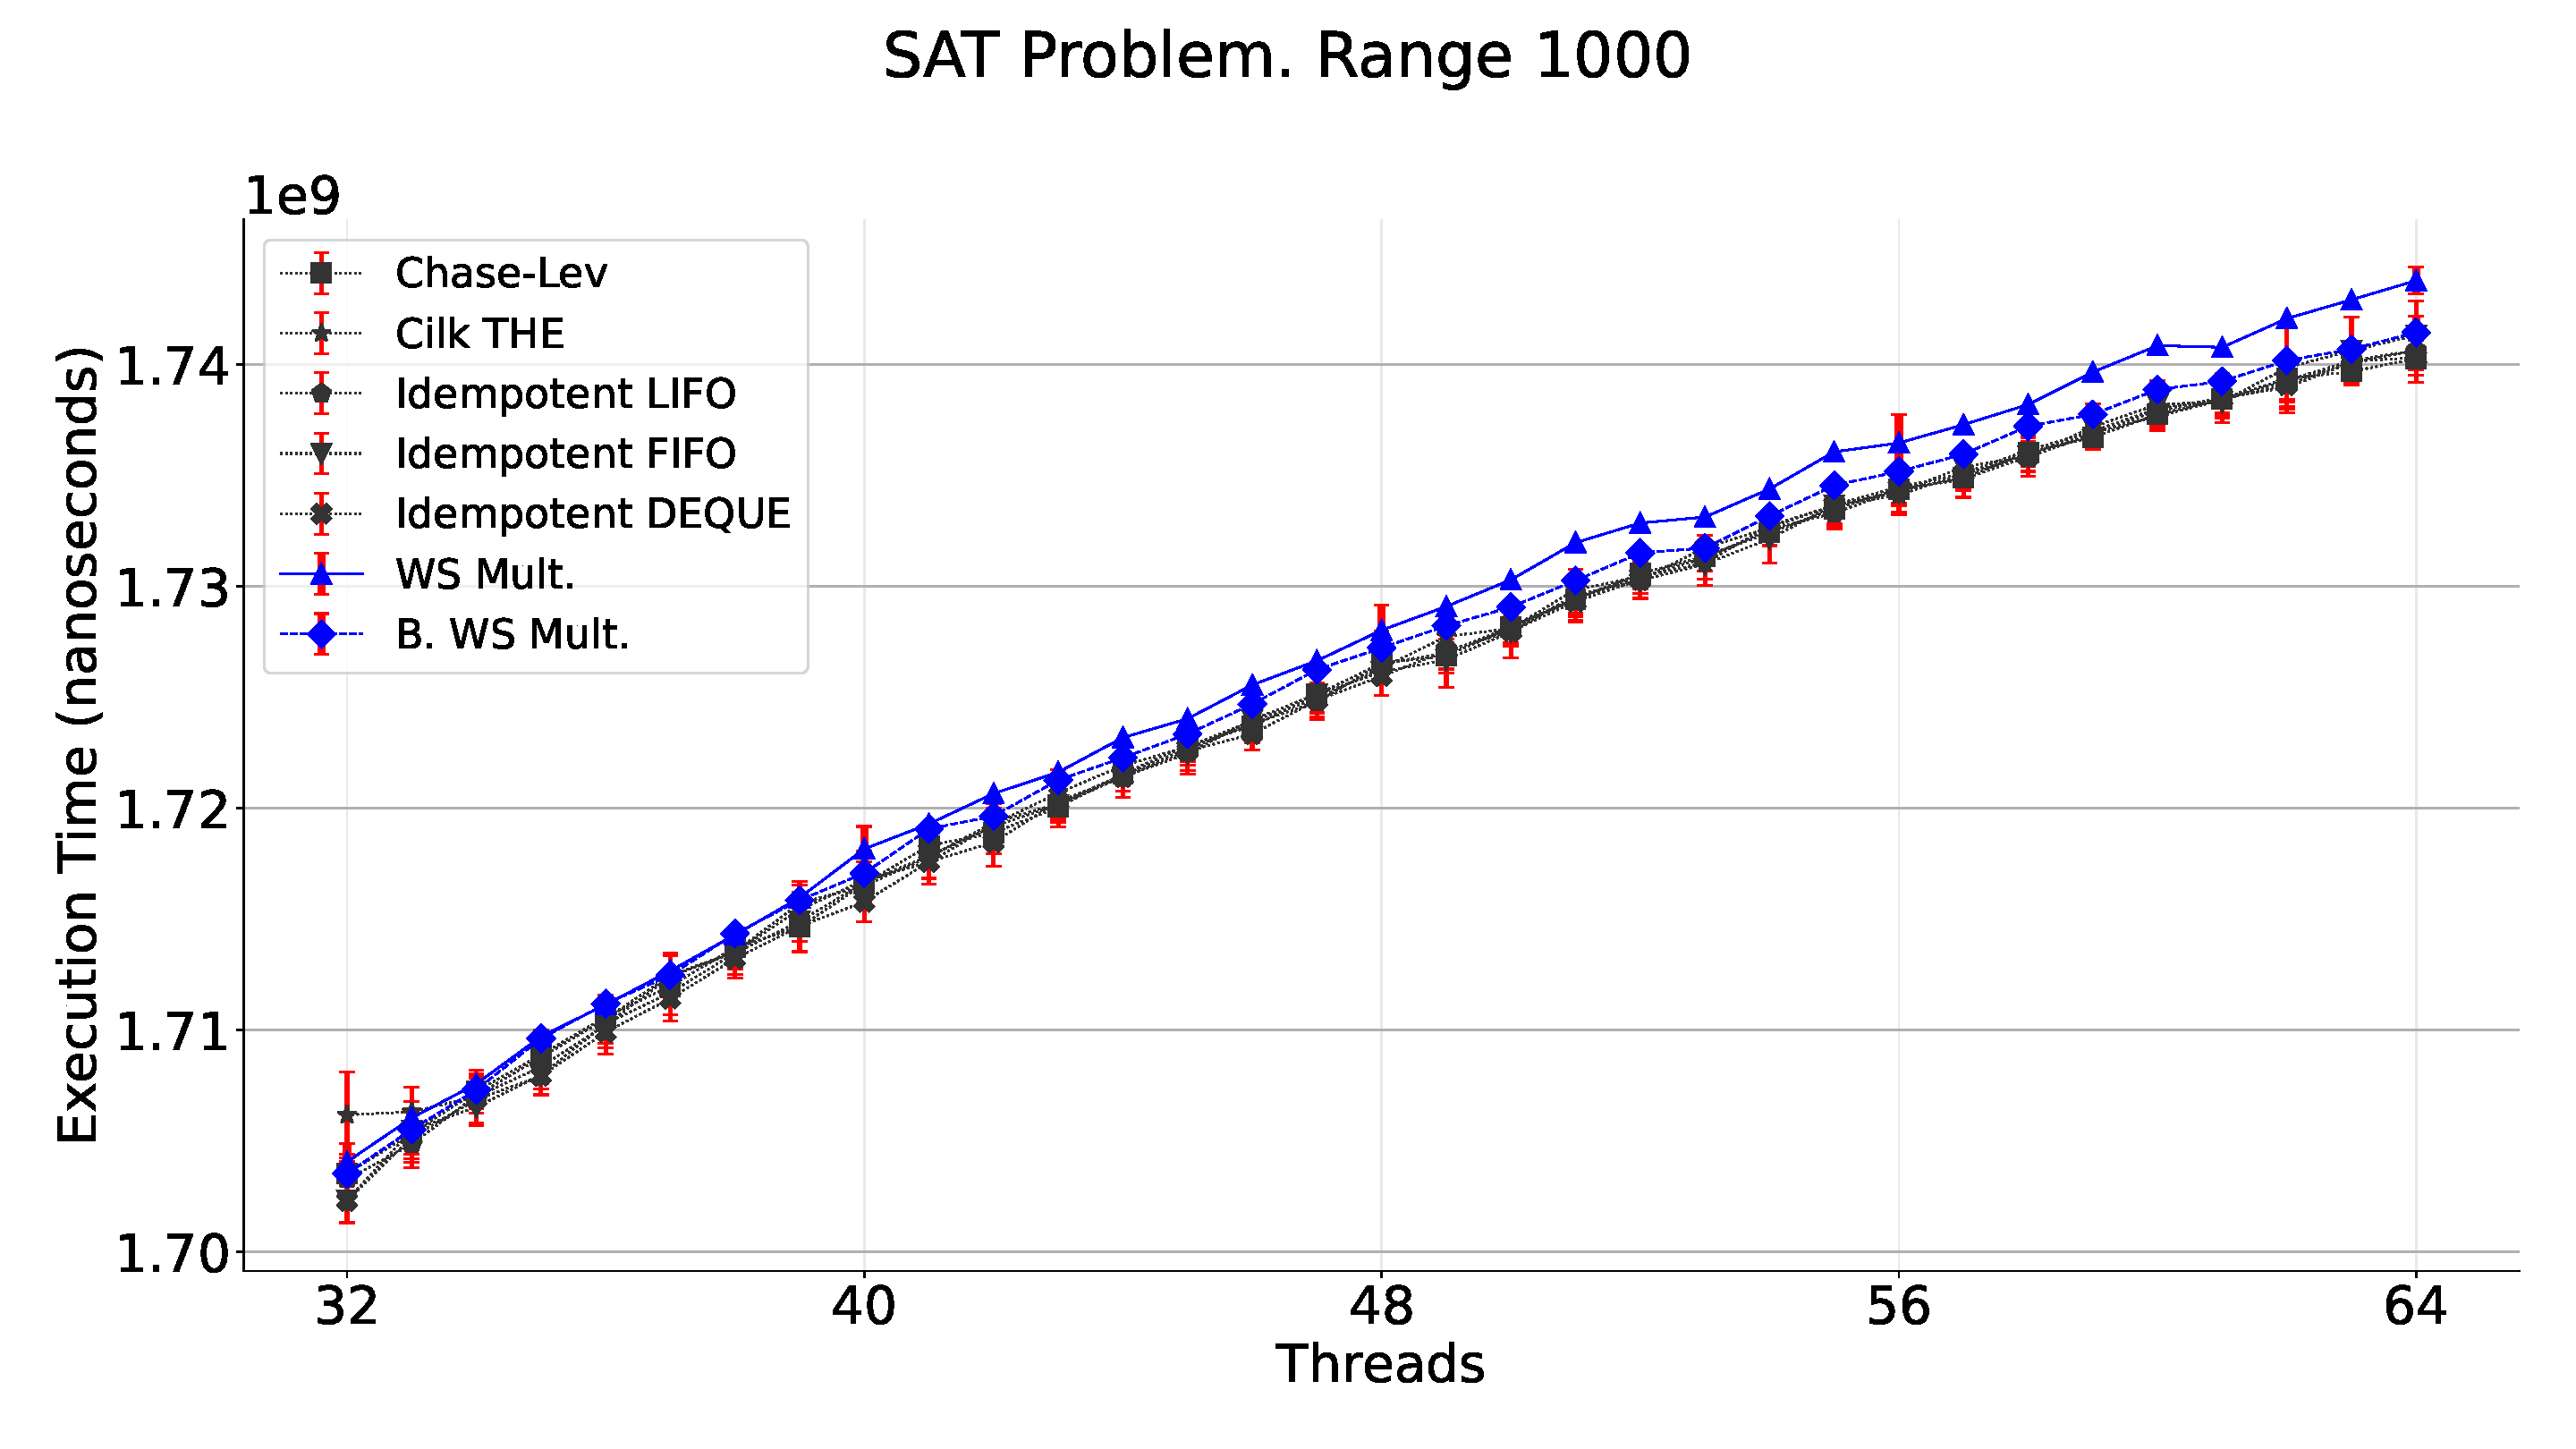
\includegraphics[width=0.48\textwidth]{contents/figures/IV_6_sat-1000-2.pdf}
  }


  \caption{\label{fig:satapplication} Mean times of the Parallel SAT benchmark for range assignment sizes 50, 250, and 1,000.}
\end{figure}

\subsubsection{Parallel SAT}

The outcomes for range assignment sizes 50, 250, and 1,000 are depicted in Figures~\ref{fig:sat:50:1},~\ref{fig:sat:250:1}, and~\ref{fig:sat:1000:1}, respectively. All algorithms speeded up sequential computation by 70\%, and generally, all performed very similarly. However, repeated work (the difference between the number of \Puts and the number of successful \Takes/\Steals) slightly impacted the performance of \NCWSM. Contrary to previous benchmarks, whose tasks are simple, tasks in this benchmark require more computation; hence, repeated work is costly. In the experiment with range size 50, \NCWSM's repeated work was larger than other algorithms, and this tendency became more pronounced as the number of processes increased. This happens because (1) a small range size increases the possibilities of concurrent \Puts/\Takes and (2) interleavings of \Puts/\Takes of \NCWSM, where multiplicity arises, are arguably not too complex. However, repeated work was always low, less than $1\%$. Still, the small amount of repeated work had some minor impact on \NCWSM's performance (see Figure~\ref{fig:sat:50:2}). For larger range sizes, 250 and 1,000, the amount of repeated work of \NCWSM decreased to almost zero (as concurrent \Puts/\Takes are less likely to happen), and hence its impact became negligible (see Figures~\ref{fig:sat:250:2} and~\ref{fig:sat:1000:2}). In contrast, idempotent algorithms had low amounts of repeated work in all cases (always close to zero), which arguably happened because the interleavings where the relaxation occurs are less likely to occur. All algorithms exhibited the same performance when the range sizes were more significant, with ranges sizes of 250 and 1,000. It is worth stressing that insert/extract policies did not affect performance, as all tasks were generated at the beginning of the experiment; hence, basically, every \Take/\Steal had to read from main memory at all times.

The outcomes of the rest of the experiments, for range assignment sizes 100, 500, and 2,500, are similar. Appendix \ref{sec:sat-appendix} contains all results of the benchmark.

%% TODO: Compilar versión con apéndice al terminar el documento.


\section{\label{sec:results-modular-basket-queue}Modular Basket Queues}

% \subsection{\label{sec:queue-experiments}Experiments}

In this section, we discuss the outcome of an experimental evaluation of the modular baskets queue algorithms presented in Chapter~\ref{chapter:5_modular-basket-queues}. To evaluate the modular queue's performance, we have designed a set of experiments that allow us to determine whether it is competitive with queues in the state-of-the-art literature. We divide our experiments into two classes: \textit{inner experiments} and \textit{outer experiments}.


Inner experiments evaluate the performance of the modular queue using distinct implementations of \LL/\IC objects and baskets. These experiments allow us to consider which implementations (combinations of LL/IC objects and baskets to build the modular queue) perform best. Also, this allows us to know if, using more relaxed objects, the queue's performance can compete with the classical synchronization objects. Once the inner experiments have been evaluated and the best combination to build the queue is chosen, we asses the selected queue against state-of-the-art queues (\textit{outer experiments}) to assess its performance and throughput. The list of queue algorithms against which we evaluate our chosen queue are:

\begin{itemize}
    \item Wait-Free queue by Yang and Mellor-Crummey~\cite{DBLP_conf_ppopp_YangM16}.
    \item Lock-Free LCRQ queue by Morrison and Afek~\cite{ppopp2013x86queues}.
    \item Lock-Free queue by Michael and Scott~\cite{DBLP_conf_podc_MichaelS96}.
    \item Lock-Free queue by Ramalhete~\cite{Ramalhete_Correia_MPMC_2016}, which was strongly inspired by the obstruction\hyp{}free queue shown in the work of Yang and Mellor-Crummey~\cite{DBLP_conf_ppopp_YangM16}
    \item Lock-Free queue by Ostrovsky and Morrison~\cite{scalingconcurrent2020}\footnote{We implemented only the version that use simple \CAS}.
\end{itemize}

\subsection{\label{subsec:queue-experimental-setup}Experimental Setup}
\subsubsection{Platforms and Implementation}

The experiments were conducted on a machine with an AMD Ryzen Threadripper 3970X processor with 64GB of memory and 32 cores, each capable of executing two hardware threads. This gives a total of 64 hardware threads for the evaluation.  We have developed the algorithms and infrastructure to carry out experimental evaluation using the C++20 programming language. This allows us to benefit from the new concurrency and parallelism features integrated with this version, including updates to atomics and synchronization facilities.

For the \textit{inner experiments} of the modular queue variants, we do not use any advanced memory reclamation protocol. Instead, we added basic memory reclamation after each evaluation. During these experiments, we only followed the specifications of the queue, \LL/\IC objects, and \textit{baskets} mentioned in Section~\ref{sec-basket-queue} to implement the distinct variants. The main objective of this experiment was to understand how different implementations of the same object (\LL/\IC, \textit{baskets}) can affect the performance of the modular queue. Below, we have provided a detailed explanation of how the experiment will be conducted.

For our \textit{outer experiments}, we use Hazard Pointers as memory reclamation for the following queues: the lock-free queue by Michael-Scott~\cite{DBLP_conf_podc_MichaelS96}, the LCRQ queue~\cite{ppopp2013x86queues}, and the lock-free queue by Ramalhete-Correia~\cite{Ramalhete_Correia_MPMC_2016}, as well as the list-of-arrays version of the modular queue. In the case of the queue by Ostrovsky-Morrison~\cite{scalingconcurrent2020} and the queue by Yang-Mellor Crummey~\cite{DBLP_conf_ppopp_YangM16}, we used their respective memory reclamation algorithms, such as epoch-based memory reclamation~\cite{DBLP_phd_ethos_Fraser04,mckenney2001read}. We followed the specifications for dynamic arrays and the list of the arrays described in Section~\ref{sec:coping-with-realistic-assumptions} to implement the modular queue for these experiments. We compared the implementations of the modular queue to the state-of-the-art queues. A detailed explanation of how the experiments are conducted is provided below.

\subsubsection{\label{subsubsec:queues-experiment-methodology}Methodology}

To evaluate the performance of the queue and its components, we conduct an experimental evaluation divided into two benchmarks. The first benchmark analyzes the \LL/\IC{} objects described in section~\ref{subsec:ll-ic-implementations} and the baskets described in section~\ref{subsec:basket-implementation}. The second benchmark evaluates the performance of the modular queue using the best \LL/\IC{} object and basket compared to queues in the state-of-the-art literature. We use the statistically rigorous methodology by Georges et al.~\cite{DBLP_conf_oopsla_GeorgesBE07}, as described in section~\ref{subsec:stat-rigor-meth}, to measure performance in both benchmarks. Each software thread is pinned to a specific hardware thread in both cases.

\subsubsection{\label{subsubsec:queue-experiments-inner-experiments}Inner Experiments}

To evaluate the performance of our distinct variants for the \LL/\IC objects and the baskets, which are fundamental for the construction of the modular queue, we perform the following experiments:

\begin{enumerate}
    \item For the case of the \LL/\IC object implementations, we conducted a test to measure the time required for executing \(5,000,000\) interspersed \LL - \IC calls to the same object by multiple threads. Each thread performs a random amount of work between \LL and \IC calls to avoid artificial long-run scenarios (see, for example,~\cite {DBLP_conf_ppopp_YangM16}). This random work consists of spinning a small amount of time (approximately six \(\mu{}s\)) in an empty loop. We took the \textit{false sharing problem}~\cite{BoloskyMichael93} into account in the array-based \LL/\IC implementations (i.e., \R/\W implementation). We tested the following versions:

    \begin{itemize}
        \item \CAS-based implementation.
        \item \R/\W-based implementation with distinct padding sizes for each array entry (0, 16, 32, 64 bytes of padding).
        \end{itemize}

We also tested the \FAI instruction in a similar setting to provide a comparison point for the \LL/\IC objects. Instead of making two calls with random work in between, we carried out \FAI with random work after its execution.

\item For the case of the combinations of \LL/\IC objects and baskets to build the modular queue, we did a similar evaluation to the previous, but testing interspersed calls to enqueue and dequeue in a shared queue by all threads. We measure the time for executing \(5\cdot 10^6\) interspersed calls to enqueue and dequeue, and similar to the previous test, we perform some artificial work to avoid artificial long-run scenarios, using the same technique described previously. The value \(K\) selected for the \(K\)-basket was \(\sqrt{N}\), with \(N\) the number of processes in the experiment. We tested the following combinations of \LL/\IC objects with the respective basket:
    \begin{itemize}
        \item \LL/\IC{} \R/\W (with padding) with \(N\)-basket
        \item \LL/\IC{} \CAS with \(N\)-basket
        \item \LL/\IC{} \R/\W (with padding) with \(K\)-basket
        \item \LL/\IC{} \CAS with \(K\)-basket
    \end{itemize}
  \end{enumerate}

\subsubsection{\label{subsubsec:queue-experiments-outer-experiments}Outer Experiments}

The previous experiment's results displayed the performance of different modular queue variations. Based on that, we selected the best LL/IC object combination with the basket for the modular queue. In this experiment, we tested three versions of that modular queue against the following queues: Yang and Mellor-Crummey's Wait-Free queue~\cite{DBLP_conf_ppopp_YangM16}, Morrison and Afek's Lock-Free LCRQ queue~\cite{ppopp2013x86queues}, Michael and Scott's Lock-Free queue~\cite{DBLP_conf_podc_MichaelS96}, Ramalhete and Correia's Lock-Free queue~\cite{Ramalhete_Correia_MPMC_2016}, which was inspired by Yang and Mellor-Crummey's obstruction-free queue-Crummey~\cite{DBLP_conf_ppopp_YangM16}, and Ostrovsky and Morrison's Lock-Free queue~\cite{scalingconcurrent2020}.

There are three versions of the modular queue: the \textit{classic version} specified in Section~\ref{sec-basket-queue}, which has a fixed size\footnote{1,000,000 of baskets} and does not have the option to resize\footnote{It is the same used for the inner experiments}; the \textit{dynamic array} version, which has an initial size of 1024 baskets and doubles its size whenever the array becomes full; and the \textit{list of arrays} version, which use Hazard Pointers[59] for memory management and utilizes nodes with basket arrays of size 1024. The last two versions are specified in Section~\ref{sec:coping-with-realistic-assumptions}.

To evaluate all the queues, we adopt a benchmark similar to that used by Ostrovsky and Morrison~\cite{scalingconcurrent2020}. This benchmark consists of three workloads: producer-only, consumer-only, and a mixed producer/consumer workload. During the experimental evaluation, each process can have the role of either a producer, who can call the \Enq function, or a consumer, who can call the \Deq function. Similar to the experiments performed in the section~\ref{subsubsec:queue-experiments-inner-experiments}, we measure the time it takes until all threads complete \(1,000,000\) operations. We use the statistically rigorous methodology described in the section~\ref{subsec:stat-rigor-meth} that follows the methodology of Georges et al.~\cite{DBLP_conf_oopsla_GeorgesBE07} for the experimental evaluation.

\subsection{Experimental Evaluation Results}

First, we present a summary of the experimental evaluation results from the Case Of Study presented in Chapter~\ref{chapter:5_modular-basket-queues}.

\paragraph*{Inner experiments (\LL/\IC evaluation)}  In this experiment, we observed that all objects had similar behavior. As expected, the \FAI instruction was faster than the \LL/\IC objects in virtually all cases. An interesting observation is that as the number of contending processes increases, the behavior of the \LL/\IC \CAS version is pretty similar to the \FAI evaluation. The \R/\W version of \LL/\IC objects behaved similarly but with lower performance than the \FAI and \CAS \LL/\IC objects. The versions using 16 and 64 bytes of padding were found to be the best.

\paragraph*{Inner experiments (Modular queue variants evaluation)} In this experiment, we observed that queues based on the \(K\)-basket are the best among all the modular queue variants. In particular, the version based on the \CAS \LL/\IC object performed the best. However, when the number of contending processes increases, it scales slightly and performs similarly. The queue using \R/\W LL/IC and the same type of basket does not scale, as shown in Figure 6.7. On the other hand, queues based on \(N\)-basket will not even be considered for more research in the future. However, it is interesting to see how the same algorithm can perform very differently using only distinct types of modules for its main parts.

\paragraph*{Outer experiments} Based on the test results, the Yang-Mellor Crummey queue is the most efficient compared to other queues. The LCRQ queue and \FAI queue are slightly less efficient than the Yang-Mellor Crummey queue. The performance of the list-of-arrays version and the classic version of the modular queue are less efficient than that of the previous three queues. However, the list-of-array version of the modular queue performs better than the original version. The Michael-Scott queue is less efficient than the previous queues. The Ostrovsky-Morrison queue performs poorly for a few processes, but its performance improves when the number of processes increases. The dynamic array version of the modular queue performs poorly, possibly due to contention when the array resizes when it becomes full.

\subsubsection{Inner Experiments - LL/IC Performance}

The outcome of the \LL/\IC performance experiments for 64 processes appears in Figure~\ref{fig:llic-times}, with their respective percentage improvement shown in Table~\ref{table:llic-percentages}. In these experiments, the only real competitor for the \FAI instruction in terms of performance was the \LL/\IC{} object \CAS-based implementation, where, in some moments, the range of improvement was over 0.46\% to 3.49\%, taking as reference the execution using the same number of processes. Nonetheless, when the number of threads was low, it showed no improvement. The Read/Write versions show a negative improvement, ranging from -3.54\% to -47.57\%. This result is expected due to additional instructions needed to execute the \LL/\IC operations. For further information about the results, refer to Appendix~\ref{sec:appendix-llic-performance} for a more detailed insight. Considering these results, we decided to test the modular queue's performance using the \CAS-based version and the \R/\W-based version with 16 and 64 bytes of padding for each entry in the next subsection.

% TODO: Actualizar apéndice.

\begin{figure}[ht!]
  \centering
  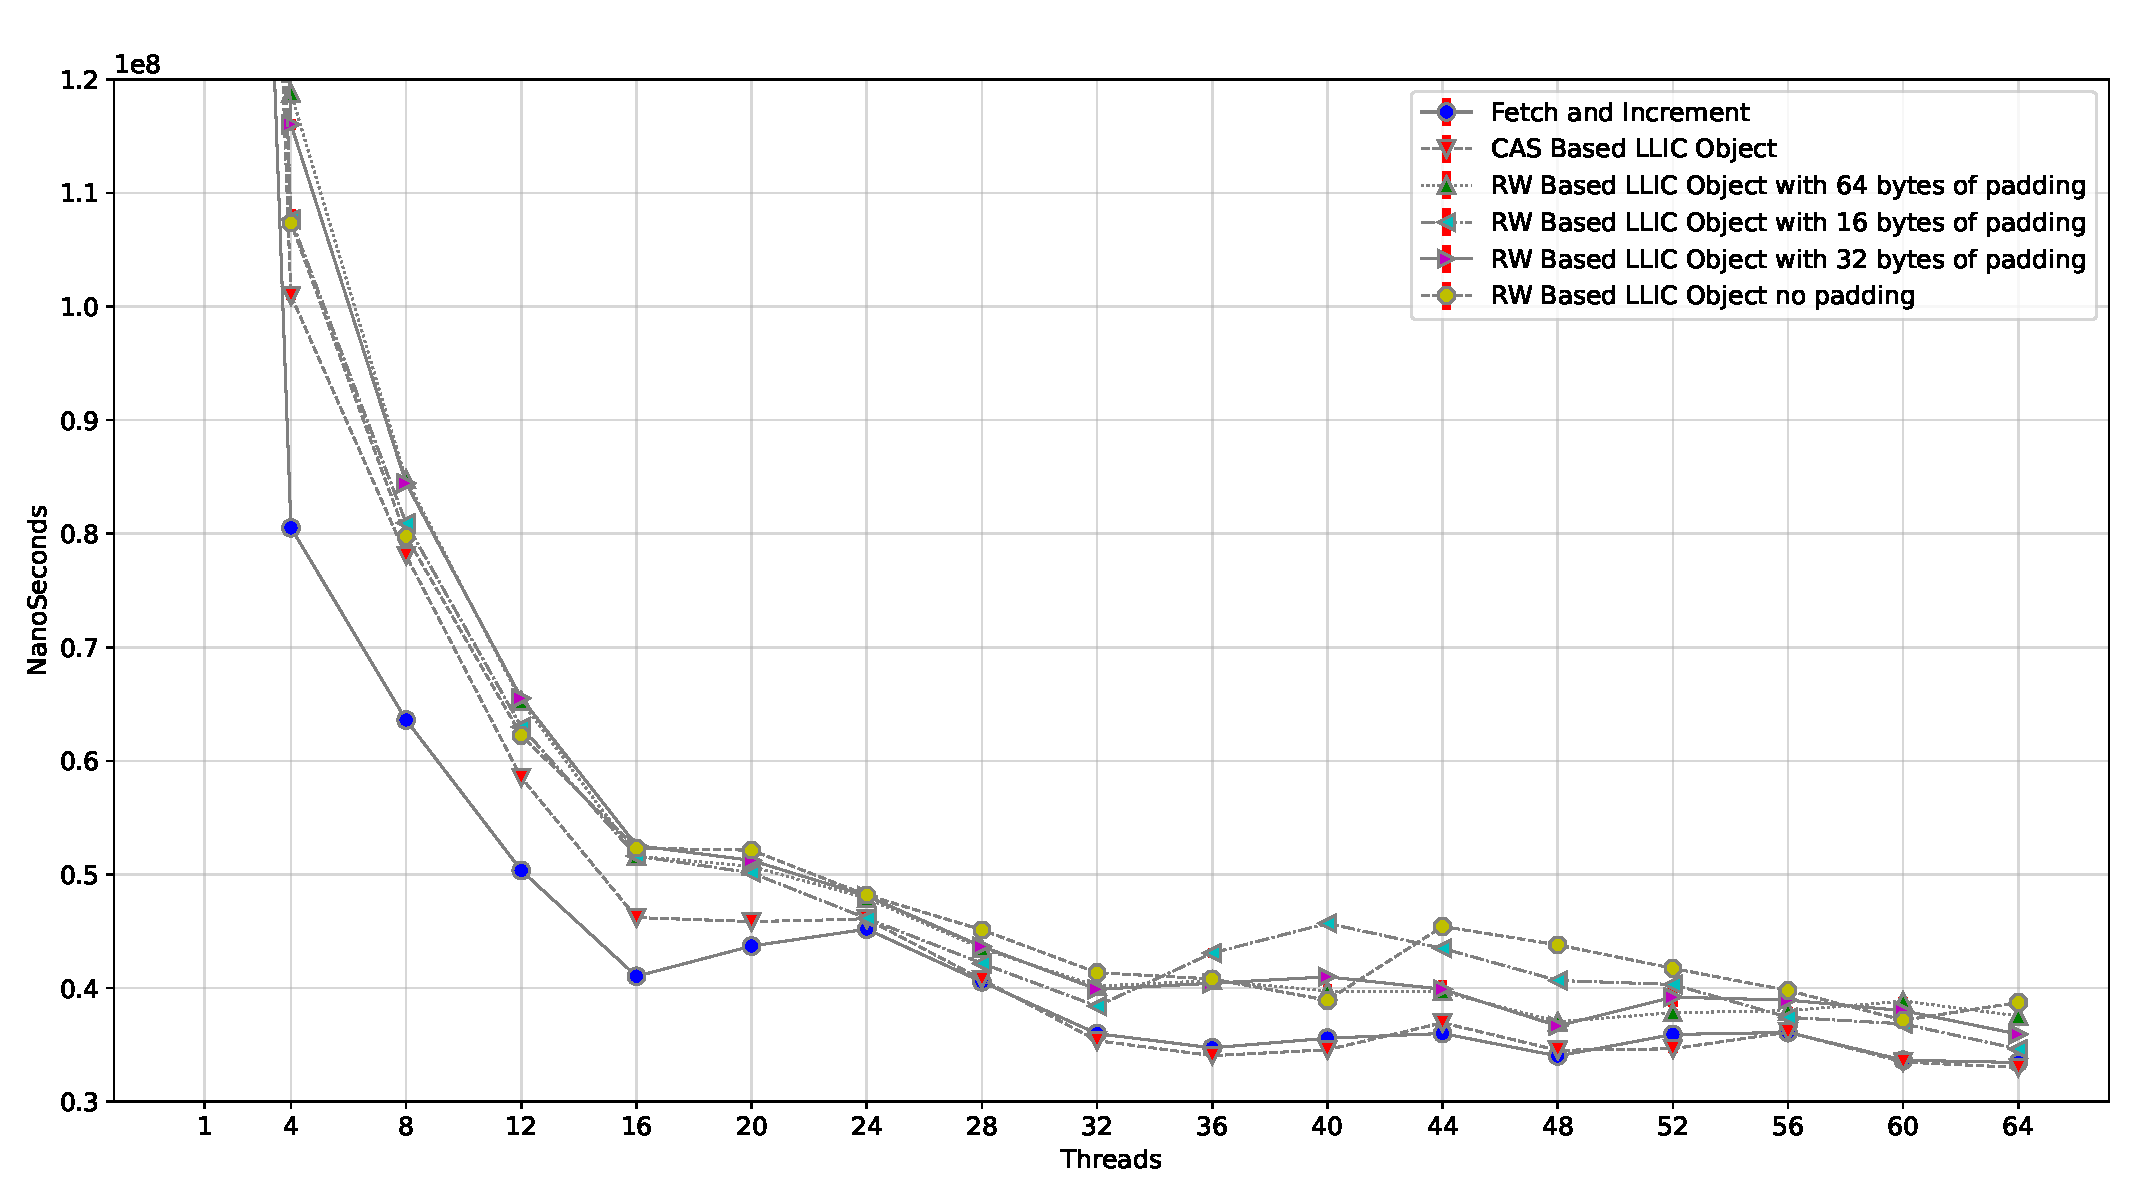
\includegraphics[width=0.9\textwidth]{contents/figures/V_llic_64_insert_extract.pdf}
  \caption{\label{fig:llic-times} Mean times for LL/IC experiment. 1,000,000 interspersed calls to \Take and \Put for 64 threads}
\end{figure}

\begin{table}[!ht]
\centering\resizebox{\textwidth}{!}{\begin{tabular}{lrrrrrr}
\toprule
 & Fetch and Increment & CAS LL/IC & RW LL/IC 64 padding & RW LL/IC 16 padding & RW LL/IC 32 padding & RW LL/IC no padding \\
\midrule
\textbf{1} & 0.00 & -5.81 & -9.76 & -10.70 & -12.23 & -10.91 \\
\textbf{8} & 0.00 & -22.76 & -33.34 & -27.24 & -32.77 & -25.41 \\
\textbf{16} & 0.00 & -12.59 & -25.75 & -25.80 & -28.05 & -27.46 \\
\textbf{24} & 0.00 & -1.96 & -6.00 & -2.10 & -6.47 & -6.61 \\
\textbf{32} & 0.00 & 1.73 & -11.61 & -6.71 & -10.84 & -14.91 \\
\textbf{40} & 0.00 & 2.86 & -11.66 & -28.41 & -15.19 & -9.38 \\
\textbf{48} & 0.00 & -1.48 & -8.85 & -19.53 & -7.78 & -28.75 \\
\textbf{56} & 0.00 & -0.05 & -5.30 & -3.68 & -7.88 & -10.23 \\
\textbf{64} & 0.00 & 1.33 & -12.25 & -3.54 & -7.44 & -15.80 \\
\bottomrule
\end{tabular}}
\caption{Percentage improvement of LL/IC objects respect to \FAI from 1 to 64 threads of execution.}
\label{table:llic-percentages}
\end{table}

% \begin{table}[!ht]
\centering\resizebox{\textwidth}{!}{\begin{tabular}{lrrrrrr}
\toprule
 & Fetch and Increment & CAS LL/IC & RW LL/IC 64 padding & RW LL/IC 16 padding & RW LL/IC 32 padding & RW LL/IC no padding \\
\midrule
\textbf{1} & 288860972.63 & 305638864.47 & 317065162.60 & 319755230.40 & 324187867.90 & 320378736.50 \\
\textbf{8} & 63599707.47 & 78075928.57 & 84805029.10 & 80927260.60 & 84444217.30 & 79758733.07 \\
\textbf{16} & 41037828.93 & 46203364.33 & 51603157.93 & 51627402.33 & 52549893.80 & 52305099.07 \\
\textbf{24} & 45187224.67 & 46074348.43 & 47896947.17 & 46134113.00 & 48109941.77 & 48176109.00 \\
\textbf{32} & 35988846.27 & 35367188.00 & 40166244.37 & 38405117.57 & 39891455.73 & 41353746.77 \\
\textbf{40} & 35586323.23 & 34568989.23 & 39735940.17 & 45696269.77 & 40990485.80 & 38923483.30 \\
\textbf{48} & 34018945.07 & 34521533.77 & 37031091.27 & 40663404.70 & 36665244.53 & 43799081.63 \\
\textbf{56} & 36094405.17 & 36113970.37 & 38005800.77 & 37420952.30 & 38938837.97 & 39787863.63 \\
\textbf{64} & 33447182.50 & 33003608.20 & 37543791.23 & 34631263.33 & 35936880.00 & 38732530.37 \\
\bottomrule
\end{tabular}}
\caption{Mean times for LL/IC experiemnt}
\label{table:llic-times}
\end{table}


\subsubsection{\label{subsec:inner-experiments}Inner Experiments - Modular Queue Variants}


The Enqueue - Dequeue Outer Experiment outcome for 64 processes appears in Figure~\ref
{fig:64-inner-enq-deq}, and their respective percentage improvements are shown in Table~\ref{table:64-inner-enq-deq-percentages}. In these experiments, we observe that our best version of the modular queue is the combination of the \CAS-based \LL/\IC object and the \(K\)-basket. In particular, all the queue versions tested based on the \(N\)-basket performed worse than those based on the \(K\)-basket. For example, taking the best version of the \(N\)-basket, which is the one that uses \LL/\IC object \CAS-based, they have a lousy performance concerning the version conformed by \LL/\IC object \CAS-based and the \(K\)-basket ranging from -1.74\% using one thread to -1229.5\% using 64 threads. The queue based on the \(N\)-basket does not scale well. We observe similar behavior in the queue based on \(N\)-basket with \R/\W \LL/\IC objects (16 and 64 bytes of padding). They also range from -0.89\% to -1356.19\% of lousy performance with respect to the performance of the queue that uses \(K\)-basket and \CAS-based \LL/\IC objects.

The queue with \(K\)-basket and \R/\W-based \LL/\IC objects also performed worse, but not so severely. Its performance ranges from -0.79\% to -281.49\% concerning using \(K\)-basket and \CAS-based \LL/\IC objects. Based on the results obtained, we have decided to test the modular queue that employs \(K\)-basket and \CAS-based LL/IC objects against the state-of-the-art queues mentioned in Section~\ref{subsubsec:queue-experiments-outer-experiments}. This queue version will be referred to as the Castañeda-Piña queue in the following section. % Section~\ref{subsec:outer-experiments}.

\begin{figure}[ht!]
  \centering
  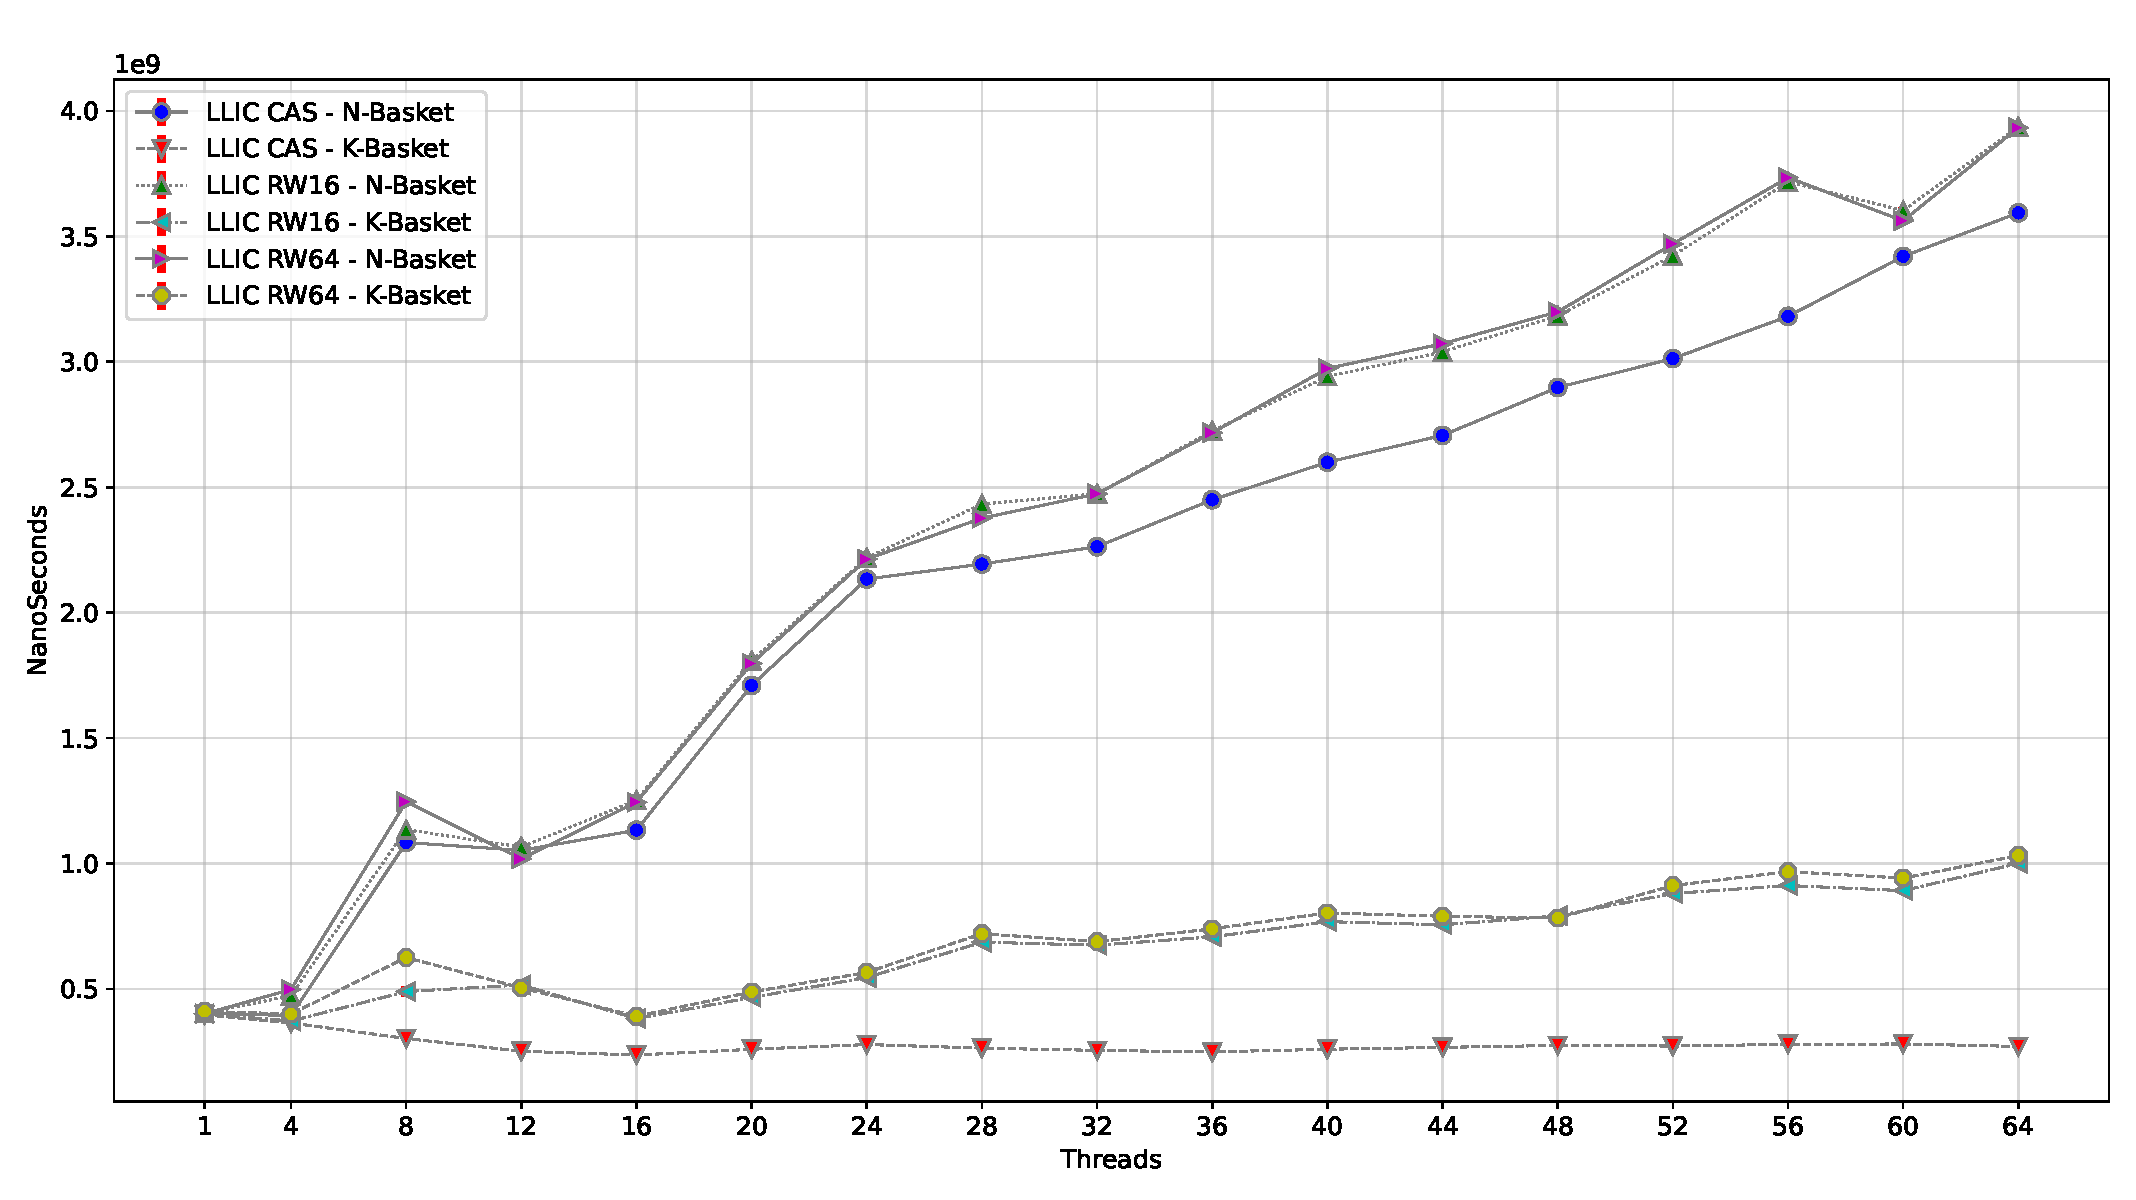
\includegraphics[width=0.9\textwidth]{contents/figures/V_64_inner_enq_deq_all.pdf}
  \caption{\label{fig:64-inner-enq-deq} Mean times for Enqueue - Dequeue in inner experiments. 1,000,000 interspersed calls to \Enq and \Deq  for 64 threads}
\end{figure}

%\begin{table}[!ht]
\centering\resizebox{\textwidth}{!}{\begin{tabular}{lrrrrrr}
\toprule
 & LLIC CAS - N-Basket & LLIC CAS - K-Basket & LLIC RW16 - N-Basket & LLIC RW16 - K-Basket & LLIC RW64 - N-Basket & LLIC RW64 - K-Basket \\
\midrule
\textbf{1} & 403837572.97 & 396923559.23 & 403364522.07 & 400055812.90 & 400458163.90 & 410361616.03 \\
\textbf{8} & 1083497864.53 & 301903826.67 & 1134626840.47 & 489293420.43 & 1246191018.60 & 624905787.60 \\
\textbf{16} & 1132563585.47 & 236075970.90 & 1252081224.87 & 381578408.67 & 1244407677.97 & 390607216.17 \\
\textbf{24} & 2133731012.70 & 278000991.57 & 2218159617.33 & 544932910.07 & 2213154726.97 & 565660003.90 \\
\textbf{32} & 2262827345.93 & 254498662.33 & 2474083071.13 & 674008201.03 & 2473843065.13 & 688144066.47 \\
\textbf{40} & 2599424591.43 & 259304569.17 & 2941545544.63 & 767947461.03 & 2973306680.03 & 802582429.10 \\
\textbf{48} & 2897334261.40 & 274293059.03 & 3183274684.97 & 791166367.20 & 3199031929.60 & 782029672.97 \\
\textbf{56} & 3181102862.03 & 278835375.93 & 3717005695.57 & 911886436.97 & 3734223566.20 & 967380566.13 \\
\textbf{64} & 3593712103.47 & 270304602.33 & 3936145887.47 & 1000239685.37 & 3933207413.67 & 1031183359.33 \\
\bottomrule
\end{tabular}}
\caption{Mean times for Enqueue - Dequeue inner experiment for 64 threads.}
\label{table:64-inner-enq-deq-times}
\end{table}

\begin{table}[!ht]
\centering\resizebox{\textwidth}{!}{\begin{tabular}{lrrrrrr}
\toprule
 & LLIC CAS - N-Basket & LLIC CAS - K-Basket & LLIC RW16 - N-Basket & LLIC RW16 - K-Basket & LLIC RW64 - N-Basket & LLIC RW64 - K-Basket \\
\midrule
\textbf{1} & -1.74 & 0.00 & -1.62 & -0.79 & -0.89 & -3.39 \\
\textbf{8} & -258.89 & 0.00 & -275.82 & -62.07 & -312.78 & -106.99 \\
\textbf{16} & -379.75 & 0.00 & -430.37 & -61.63 & -427.12 & -65.46 \\
\textbf{24} & -667.53 & 0.00 & -697.90 & -96.02 & -696.10 & -103.47 \\
\textbf{32} & -789.13 & 0.00 & -872.14 & -164.84 & -872.05 & -170.39 \\
\textbf{40} & -902.46 & 0.00 & -1034.40 & -196.16 & -1046.65 & -209.51 \\
\textbf{48} & -956.29 & 0.00 & -1060.54 & -188.44 & -1066.28 & -185.11 \\
\textbf{56} & -1040.85 & 0.00 & -1233.05 & -227.03 & -1239.22 & -246.94 \\
\textbf{64} & -1229.50 & 0.00 & -1356.19 & -270.04 & -1355.10 & -281.49 \\
\bottomrule
\end{tabular}}
\caption{Percentage improvement of Enqueue - Dequeue respect to LL/IC \CAS \& K-Basket from 1 to 64 threads of execution.}
\label{table:64-inner-enq-deq-percentages}
\end{table}



\subsubsection{\label{subsec:outer-experiments}Outer Experiments}

The outcome of the Enqueue - Dequeue Outer Experiment for 64 processes appears in Figure~\ref{fig:64-outer--enq-deq}, and their respective percentage improvement is shown in Table~\ref{table:64-outer-enq-deq-percentages}. In these experiments, we observe that Yang-Mellor Crummey's queue performed best in almost every execution, followed closely by Ramalhete's \FAI queue (\FAI queue) and the LCRQ queue.


Their graphs look very similar; however, for executions using few cores occasionally, LCRQ and the \FAI queues have some improvements over the performance of the Yang-Mellor Crummey queue. The \FAI queue in some executions has an improvement ranging from 0.87\% to 6.92\%, but after 16 threads, its improvements begin to descend, ranging from -5.59\% to -50.75\%. LCRQ's negative improvement ranged from -6.96\% to -193.12\%. In some moments, its improvement grows up to 5.61\%.


\begin{figure}[ht!]
  \centering
  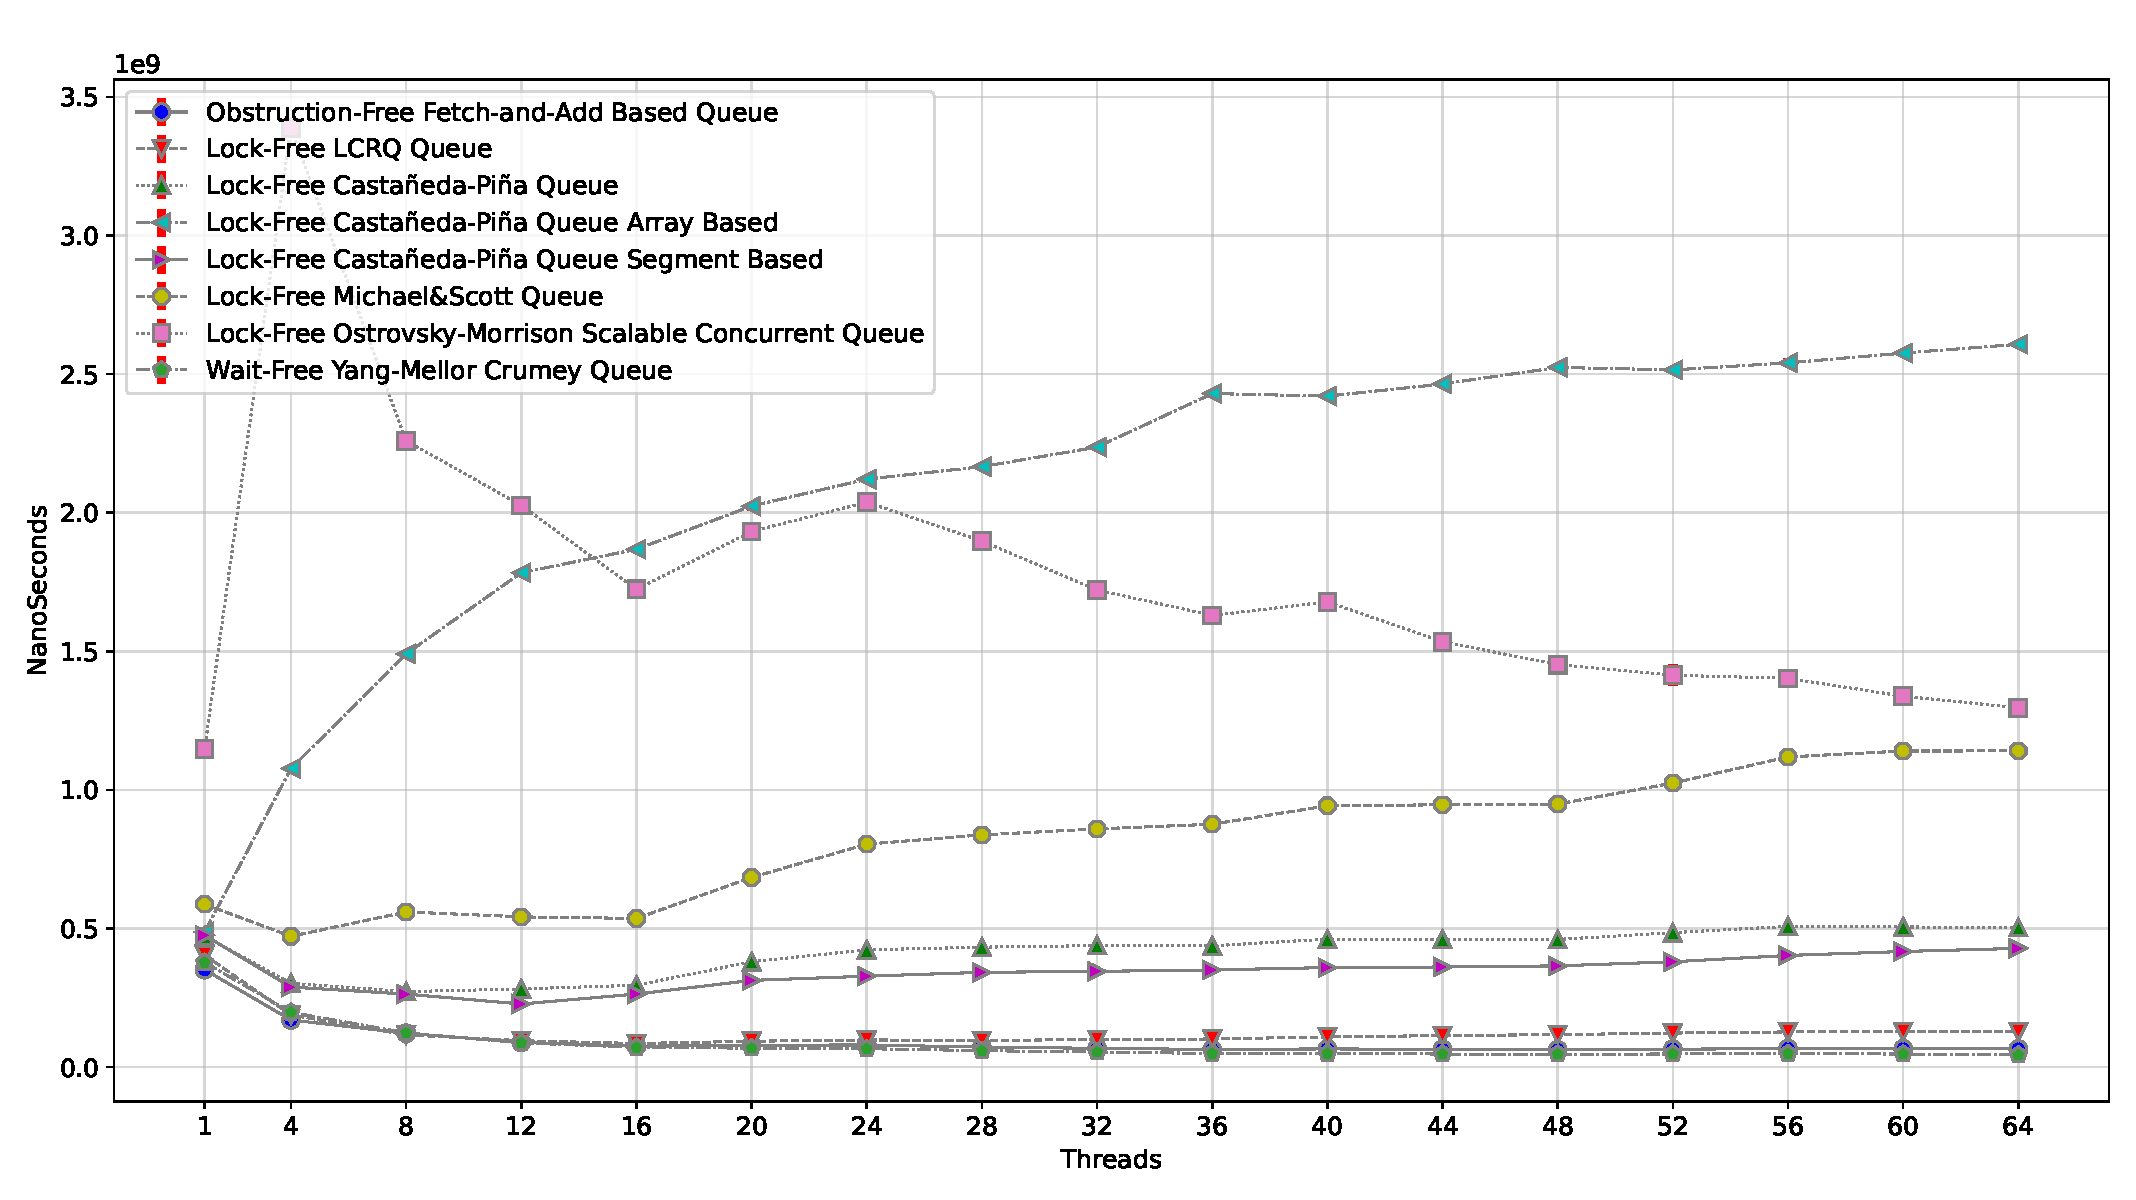
\includegraphics[width=0.9\textwidth]{contents/figures/V_64_outer_enq_deq_all.pdf}
  \caption{\label{fig:64-outer--enq-deq} Mean times for Enqueue - Dequeue in outer experiments. 1,000,000 interspersed calls to \Enq and \Deq  for 64 threads}
\end{figure}

According to performance analysis, the Castañeda-Piña list of arrays and its classic versions are the following queues that perform better among all queues. Although their overall performance is similar, the list-of-arrays version outperforms the classic version. The classic version shows a negative improvement ranging from -25.25\% to -1063.06\%, whereas the list-of-array version ranges from -26.03\% to -890.09\%, both of which are inferior to Yang-Mellor Crummey's queue. However, they perform better than other reported queues, as illustrated in Figure~\ref{fig:64-outer--enq-deq}. A reason the list of arrays performed better than the classic is due to the allocation/deallocation of small pieces of memory instead of big chunks, like in the classic version.


%\begin{table}[!ht]
\centering\resizebox{\textwidth}{!}{\begin{tabular}{lrrrrrrrr}
\toprule
 & Fetch-and-Add & LCRQ & Castañeda-Piña & Castañeda-Piña Array & Castañeda-Piña Segments & Michael and Scott & Ostrovsky-Morrison & YMC \\
\midrule
\textbf{1} & 351200027.63 & 403572408.43 & 472555550.90 & 487165396.30 & 475511479.40 & 587248865.70 & 1146251708.13 & 377297171.80 \\
\textbf{8} & 121854879.07 & 116026264.60 & 272038021.70 & 1490503277.57 & 263046870.43 & 559538345.73 & 2259382162.50 & 122918448.70 \\
\textbf{16} & 74776242.40 & 84622830.50 & 294978630.73 & 1867961323.20 & 263256036.93 & 535908982.53 & 1723493401.93 & 70816962.53 \\
\textbf{24} & 79543299.43 & 97720927.97 & 422919854.07 & 2120916067.10 & 327654824.50 & 803985551.10 & 2037756243.03 & 66012273.80 \\
\textbf{32} & 67443713.50 & 99412632.57 & 438538137.47 & 2236554396.10 & 345087614.40 & 859154816.23 & 1720945612.37 & 53669770.97 \\
\textbf{40} & 65311551.40 & 108716588.03 & 461605337.17 & 2420424604.93 & 358781500.57 & 942633485.97 & 1678287663.47 & 48899447.00 \\
\textbf{48} & 62148500.10 & 116865624.87 & 460302515.57 & 2523987255.27 & 364872124.93 & 948736421.87 & 1451514990.13 & 46240439.33 \\
\textbf{56} & 66547657.57 & 126754099.80 & 507507288.80 & 2540588509.17 & 402499664.00 & 1118652395.07 & 1402048064.73 & 47973167.30 \\
\textbf{64} & 65178512.30 & 126730354.90 & 502870762.67 & 2607573629.43 & 428069875.03 & 1140572453.10 & 1295963945.30 & 43235588.63 \\
\bottomrule
\end{tabular}}
\caption{Mean times for Enqueue - Dequeue outer experiment for 64 threads.}
\label{table:64-outer-enq-deq-times}
\end{table}

\begin{table}[!ht]
\centering\resizebox{\textwidth}{!}{\begin{tabular}{lrrrrrrrr}
\toprule
 & Fetch-and-Add & LCRQ & Castañeda-Piña & Castañeda-Piña Array & Castañeda-Piña Segments & Michael and Scott & Ostrovsky-Morrison & YMC \\
\midrule
\textbf{1} & 6.92 & -6.96 & -25.25 & -29.12 & -26.03 & -55.65 & -203.81 & 0.00 \\
\textbf{8} & 0.87 & 5.61 & -121.32 & -1112.60 & -114.00 & -355.21 & -1738.11 & 0.00 \\
\textbf{16} & -5.59 & -19.50 & -316.54 & -2537.73 & -271.74 & -656.75 & -2333.73 & 0.00 \\
\textbf{24} & -20.50 & -48.03 & -540.67 & -3112.91 & -396.35 & -1117.93 & -2986.94 & 0.00 \\
\textbf{32} & -25.66 & -85.23 & -717.10 & -4067.25 & -542.98 & -1500.82 & -3106.55 & 0.00 \\
\textbf{40} & -33.56 & -122.33 & -843.99 & -4849.80 & -633.71 & -1827.70 & -3332.12 & 0.00 \\
\textbf{48} & -34.40 & -152.73 & -895.45 & -5358.40 & -689.08 & -1951.75 & -3039.06 & 0.00 \\
\textbf{56} & -38.72 & -164.22 & -957.90 & -5195.85 & -739.01 & -2231.83 & -2822.57 & 0.00 \\
\textbf{64} & -50.75 & -193.12 & -1063.09 & -5931.08 & -890.09 & -2538.04 & -2897.45 & 0.00 \\
\bottomrule
\end{tabular}}
\caption{Percentage improvement of Enqueue - Dequeue respect to Yang and Mellor-Crummey Queue from 1 to 64 threads of execution.}
\label{table:64-outer-enq-deq-percentages}
\end{table}


It has been observed that the Michael-Scott and Ostrovsky-Morrison queues have underperformed compared to the previous queues. In the case of Michael-Scott's queue, we noticed a decline in performance ranging from -55.65\% to -2,538.04\% compared to Yang-Mellor Crummey's queue. However, the decline in performance is consistent with the increase in the number of threads.

Similarly, for Ostrovsky-Morrison's queue, the performance deteriorates as the number of threads increases. For instance, the performance for one thread was found to be close to -55\% as compared to Yang-Mellor Crummey's queue using one thread as well. However, when the number of threads increased from 4 to 32, we observed a further decline in performance ranging from -1738\% to -3106\%. After this number of threads, the performance improvement began to reduce until it reached a value close to -2807\% compared to the performance of Yang-Mellor Crummey's queue for the same number of threads.

The Castañeda-Piña queue using dynamic arrays had the worst overall performance, exhibiting a non-scalable behavior that only increases in time as the number of threads increases, ranging from -29.12\% to -5931.08\%. A possible reason for the bad performance is the time it takes to double its size and the contention while this operation is performed.

%%% Local Variables:
%%% mode: LaTeX
%%% TeX-master: "../../main"
%%% End:
